\documentclass[12pt, a4paper, bibliography=totoc, english]{scrartcl}
\usepackage[T1]{fontenc}
\usepackage[utf8]{inputenc}
\usepackage[american]{babel}
\usepackage{listings} 
\usepackage{xcolor} 
\usepackage{colordef}
\usepackage{lvblisting}
\usepackage{graphicx}
\usepackage{hyperref}
\usepackage{geometry}
\geometry{letterpaper}
\usepackage{amssymb}

\usepackage{tocbibind}
\usepackage[section]{placeins}
\usepackage{float}

\usepackage[
left=2cm,
right=3cm,
top=2.5cm,
bottom=2cm,	
]{geometry}



\usepackage{csquotes}
\usepackage[backend=biber, 
style=apa,
sorting=nyt,
maxnames=2,
minnames=1,
maxbibnames=99,
uniquename=false,
uniquelist=false,
citestyle=authoryear,
block=space,
]{biblatex}
\addbibresource{litnew.bib}
\DeclareLanguageMapping{american}{american-apa}

\setlength\bibitemsep{1.5\itemsep}

\renewbibmacro*{name:last-first}[4]{%
	\ifuseprefix
	{\usebibmacro{name:delim}{#3#1}%
		\usebibmacro{name:hook}{#3#1}%
		\ifblank{#3}{}{%
			\ifcapital
			{\mkbibbold{\mkbibnameprefix{\MakeCapital{#3}}\isdot}}
			{\mkbibbold{\mkbibnameprefix{#3}\isdot}}%
			\ifpunctmark{'}{}{\bibnamedelimc}}%
		\mkbibbold{\mkbibnamelast{#1}\isdot}%
		\ifblank{#4}{}{\bibnamedelimd\mkbibnameaffix{#4}\isdot}%
		\ifblank{#2}{}{\revsdnamepunct\bibnamedelimd\mkbibnamefirst{#2}\isdot}}
	{\usebibmacro{name:delim}{#1}%
		\usebibmacro{name:hook}{#1}%
		\mkbibbold{\mkbibnamelast{#1}\isdot}%
		\ifblank{#4}{}{\bibnamedelimd\mkbibnameaffix{#4}\isdot}%
		\ifblank{#2#3}{}{\revsdnamepunct}%
		\ifblank{#2}{}{\bibnamedelimd\mkbibnamefirst{#2}\isdot}%
		\ifblank{#3}{}{\bibnamedelimd\mkbibnameprefix{#3}\isdot}}}

\usepackage{tocloft}
\renewcommand{\cftsecleader}{\cftdotfill{\cftdotsep}}


\usepackage[pdftex]{graphicx}

\usepackage[pdfpagelabels,  % logische (z.b. auch roemische) seitenzahlen
bookmarks,       % Bookmarks für die einzelnen Abschnitte
pdftex
]{hyperref}
\hypersetup{
	%   colorlinks,  % Links mit farbigem Text
	pdfborder   = 0 0 0,
	plainpages  = false,
	bookmarksnumbered = true,
	pdftitle    = {},
	pdfsubject  = {Case Study},
	pdfauthor   = {Hauke Pengel},
	%pdfkeywords = {Roboterassistierte Chirurgie, Laserosteotomie, optischer Kohärenztomographie,
	%Ablationsüberwachung},
	%   bookmarksopen
}


\usepackage[onehalfspacing]{setspace}

\usepackage{titlesec} %Abstand vor und nach section-Überschriften einstellen

\titlespacing*{\section}
{0pt}{5.5ex plus 1ex minus .2ex}{4.3ex plus .2ex}
\titlespacing*{\subsection}
{0pt}{5.5ex plus 1ex minus .2ex}{4.3ex plus .2ex}
\titlespacing*{\subsubsection}
{0pt}{5.5ex plus 1ex minus .2ex}{4.3ex plus .2ex}


\newcommand*{\SignatureAndDate}[1]{%
	\par\noindent\makebox[2.5in]{\hrulefill} \hfill\makebox[2.0in]{\hrulefill}%
	\par\noindent\makebox[2.5in][l]{#1}      \hfill\makebox[2.0in][l]{Date}%
}%


\usepackage{mathrsfs, amssymb} %Paket für Mathe-Formeln
\usepackage{amsmath}
\usepackage{theorem}
\DeclareMathAlphabet{\mathcal}{OMS}{cmsy}{m}{n}


\title{Title}
\author{Jingyi Liu}
\date{\today}

\begin{document}
	
	\begin{titlepage}

\begin{center}


% Oberer Teil der Titelseite:
\begin{figure}


\includegraphics[scale=0.7]{hukombi_bwb.pdf}\\   

\end{figure}


%\textsc{\LARGE University}\\[1.5cm]

%\textsc{\Large Bachelor Thesis (12 weeks)}\\[0.5cm]


% Title
\newcommand{\HRule}{\rule{\linewidth}{0.5mm}}
\HRule \\[0.02cm]
{ \huge \bfseries \begin{onehalfspace}
Use Machine Learning Methods In Bank Marketing
\end{onehalfspace}}

{ \large \bfseries \begin{onehalfspace}
Statistical Programming Language
\end{onehalfspace}}

\HRule \\[0.8cm]

%\textsc{\Large Chair of Microeconomics}\\[1cm]

% Author and supervisor
\begin{minipage}{0.4\textwidth}
\begin{flushleft} \large
\emph{Authors:}\\
Zhou \textsc{Ren}\\
Jingyi \textsc{Liu}\\
Manqi \textsc{Ding}\\
Jiayin \textsc{Yuan}
\end{flushleft}
\end{minipage}
\hfill
\begin{minipage}{0.5\textwidth}
\begin{flushright} \large
\emph{Matriculation Number:} \\
585976\\
585921\\
585964\\
586368
\end{flushright}
\end{minipage}\\[1cm]

% Author and supervisor
%\begin{minipage}{0.4\textwidth}
%\begin{flushleft} \large
%\emph{Address:}\\
%Spithal 1a \textsc{}\\
%29468 Bergen\\
%\end{flushleft}
%\end{minipage}
%\hfill
%\begin{minipage}{0.5\textwidth}
%\begin{flushright} \large
%\emph{Place of Birth:} \\
%Uelzen \textsc{}
%\end{flushright}
%\end{minipage}\\[1cm]


\vfill

% Unterer Teil der Seite
{\large \today}

\end{center}

\end{titlepage}

	
	\clearpage
	
	\pagenumbering{Roman}
	\setcounter{page}{2}
	
	\tableofcontents
	
	\clearpage
	
	\listoffigures
	
	\clearpage
	
	\listoftables
	
	\clearpage
	
	\pagenumbering{arabic} 
	\setcounter{page}{5}
	
	
	
	\section{Introduction}\label{Intro}
	In last few years, more and more decision making relied on data, so now people want to extract more knowledge from large amounts of data ,data mining plays a key role in this process. Our statistical issue is using data mining methods, especially machine learning methods, try to  predict the success of telemarketing calls for selling bank long-term deposits.
	
	The basis of our work is Sergio Moro, Paulo Cortez and Paulo Rita's paper in 2014, they used data mining approach to predict the success of bank telemarketing.According to the ideas they proposed, the procedure they implemented and the result they got, we try to replicate their whole data mining process and extend to use more analysis methods.
	
	
	In the reference paper, the authors use four classification models to predict.In our simulation,  six classification models used by us to predict.Including the classical statistical model like classical logistic regression and decision tree, which are easy to understand while have good prediction results. Furthermore, we implement four ``black box'' models to predict, include random forest, neural network, support vector machines and ensemble selection.These ``black box'' models are complex and hard to understand but in general they have higher and more stable accuracy than classical statistical model.The most special model is ensemble selection.This model is the integration of other models, it can generate all ``black box'' models, compare them and make a robust linear combination of models using a GLM. 
	
	Previous studies have shown that models have different performances in different situation, there is not one model always outperform others. So comparison is an essential step.We evaluate models through the ROC graphics and AUC values.The ROC (receiver operating characteristic) is created by plotting the true positive rate(TPR) against the false positive rate (FPR) at various threshold settings, the AUC(area under curve) provides the value of accuracy which can be calculated by the area under ROC curve, the perfect prediction have the AUC of 1. ROC  and AUC analysis provide tools to select possibly optimal models.
	
	The data of our work are collected from a Portuguese retail bank, from May 2008 to Nov 2010. We download the data and the reference paper from the UCI machine learning repository. The used data have 41188 examples and each have 20 inputs, ordered by date (from May 2008 to November 2010), very close to the data analyzed in reference paper. The output is to predict if the client will subscribe (yes/no) a term deposit (variable y). Furthermore, we also write codes about how to add quarterly socio-economic variable to the original data for adding inputs, the socio-economic variable are downloaded from the statistical center of Portuguese central bank.
	
	\section{Theory of Models}\label{Th}
	\subsection{Logistic Regression}
	In statistics, logistic regression is a classical regression model where the dependent variable is categorical, is very appropriate to be applied in our project whose outcomes ($y$) are binary. Logistic regression involves a more probabilistic view of classification, it helps to solve classification problem. In our case, a binary logistic model is used to predict whether a potential client will buy a long-term bank deposit.
	
	Specifically speaking, we try to come up with a logistic function first. The logistic function can take any real input $Z$, whereas the output always takes values between 0 and 1 and hence is interpretable as a probability. The logistic function is shown below. Assume we have d units of observed independent variables, the model consists of a vector $\beta$ in d-dimensional feature space. In vector form for a linear regression model our prediction is equal to transpose of $\beta$ vector multiplied by input parameter vector $X$.
	\begin{center}
		$\rho=\dfrac{1}{1+e^{-z}}$\vspace{3mm}
		\\
		$z=\alpha+$ $\beta{\cdot}X$$=\alpha+\beta_1{\cdot}x_1+\beta_2{\cdot}x_2+\cdots+\beta_x{\cdot}x_x$\vspace{3mm}
	\end{center}
	Using a logistic regression model, we can predict the binary outcome by applying threshold to probability. In our implement, we use the entire database as training data and testing data as well, aiming to provide a simplified and easy-understood analysis.
	
	\subsection{Decision tree}\label{DT}
	In decision analysis, a decision tree can be used to visually and explicitly represent decisions and decision making. The general motive of using Decision Tree is to create a training model which can use to predict class or value of target variables by learning decision rules inferred from prior training data. A decision tree is a simple representation for classifying examples, our tree model is a classification tree due to those discrete set of values. After visualization of the model, we can see its structure clearly, leaves of the tree is labeled with a class or a probability distribution over the classes while each internal node of the tree corresponds to an input feature. 
	
	Decision Tree's algorithm is in this way, first, place the best attribute of the dataset at the root of the tree, second, split the training set into subsets. Subsets should be made in such a way that each subset contains data with the same value for an attribute. Repeat the first step and second step on each subset until you find leaf nodes in all the branches of the tree. The primary challenge in the decision tree implementation is to identify which attributes do we need to consider as the root node and each level. Handling this is known the attributes selection. The popular attribute selection measures are Information gain and Gini index. 
	
	
	\subsection{Neural Network}\label{NN}
	Artificial neural networks are computing systems inspired by the biological neural network that constitute animal brains.An artificial network consists of a pool of simple processing units(neurons) which communicate by sending signals to each other over a large number of weighted connections.
	
	To each of the synapses, a weight is attached indicating the effect of the corresponding neuron, and all data pass the neural network as signals. The signals are processed first by the so-called integration function combining all incoming signals and second by the so-called activation function transforming the output of the neuron.This process likes logistic regression.The activation function f is usually a bounded nondecreasing nonlinear and differentiable function such as the logistic function  $f(z)=\dfrac{1}{1+e^{-z}}$
	
	The simplest multi-layer perceptron (also known as perceptron) consists of an input layer with n covariates and an output layer with one output neuron. It calculates the function:
	\begin{center}
		$o(x)=f(w_0+\sum_{i=1}^n {w_ix_i})=f(w_0+W^{T}X)$
		\vspace{3mm}
	\end{center}
	
	where $w_0$ denotes the intercept, $W = (w_1,\cdots,w_n)$ the vector consisting of all synaptic weights without the intercept, and $X = (x_1,...,x_n)$ the vector of all covariates. The function is mathematically equivalent to that of GLM with link function $f^{-1}$. Therefore, all calculated weights are in this case equivalent to the regression parameters of the GLM.
	
	To increase the modeling flexibility, hidden layers can be included. However, Hornik et al. (1989) showed that one hidden layer is sufficient to model any piecewise continuous function. Such an MLP with a hidden layer consisting of $J$ hidden neurons calculates the following function:\\}
$$o(x)=f(w_0+\sum_{j=1}^J {w_i {\cdot} f(w_{0j}+\sum_{i=1}^n{w_{ij}x_i})})=f(w_0+\sum_{j=1}^J {w_i {\cdot} f(w_{0j}+W_j^{T}X))}$$

where $w_0$ denotes the intercept of the output neuron and $w_{0j}$ the intercept of the $j$th hidden neuron. Additionally, $w_j$ denotes the synaptic weight corresponding to the synapse starting at the $j$th hidden neuron and leading to the output neuron, $w_j = (w_{1j},\cdots,w_{nj})$ the vector of all synaptic weights corresponding to the synapses leading to the $j$th hidden neuron, and $x= (x_1,\cdots,x_n)$ the vector of all covariates. This shows that neural networks are direct extensions of GLMs.

Neural networks are fitted to the data by learning algorithms during a training process. Package $neuralnet$ focuses on supervised learning algorithms, and we choose the widely used learning algorithm, resilient backpropagation algorithm, in our implementation. 

\subsection{Random Forest}\label{RF}
Random Forest (RF) is an ensemble and supervised learning method which is constructed with the decision tree. The most important difference from decision tree is that RF operates in a greed fashion by growing a large number of decision trees at training time.  As its name, a large number of trees construct the forest. By averaging a multitude of decision trees, RF reduces the variance and solves the over-fitting problem which caused by decision tree learning method. Another basic but important idea is randomness. One is choosing the data from the original training data set randomly, the other is selecting the input variables randomly at each node. The classification result chooses the category that obtains the majority vote in the forest. With the development and improvement of the RF, the basic algorithms consist of decision tree learning, random subspace method, tree bagging and Extra-Trees. 
The procedures of RF are processed as follows:\\
1.   Set the number of the trees as the number we require, namely $N$. \\
2.   For each tree, the data is chosen with replacement randomly from the original training set. \\
3.   Set the number of all input variables is $M$.\\
4.   For each tree, the input variables at each node are chosen randomly from all input variables, and the number of chosen variables at each node is m, obviously $m < M$. One of the chosen variables $(m)$ at each node become the split variable which builds on the entropy and information gain rule. \\
5.   Based on procedure 2-4, we have built one tree. For constructing N trees, repeating the procedures 2-4 $N$ times.\\
As for the test, each new example will run through all the $N$ trees in the modelled forest above. The majority result among the N trees will become the final foresting output. 

\subsection{Support Vector Machine}\label{SVM}

Support Vector Machine(SVM) is a supervised machine learning model for classification and regression.  An SVM model is a representation of the examples as points in space, the basic idea is to find a best hyperplane which can divide all examples into two separate categories for the binary classification. New examples are forecasted to a category based on which side of the hyperplane they fall. The hyperplane is supposed to make the margin of the closest points among the two categories as wide as possible, the points on the margin are called support vector. The hyperplane is located at the middle of the margin.  When the number of the variables is 2, hyperplane is a line. It's hard to imagine the hyperplane when the number of the variables is above 4.  When the distribution of the examples is non-linear, SVM model will project the examples into higher dimension by using Radial Basis Function (RBF) as a kernel.  By using RBF in SVM model, the combination of two parameters, gamma and cost, will influence the outcome. It will be shown in the simulation part.  

\subsection{Ensemble Selection}\label{ES}
Ensemble selection is rather a method than a model. The basic idea is to combine the results of several good models by weighted averaging or voting to makes the final result better.
The procedures of ensemble selection are processed by the following orders:\\
1.	Build a model library, which contains all the predictive models needed in the later process.\\
2.	Create a empty ensemble for further use.\\
3.	Select the model which has the highest accuracy or the best performance depending on the metrics to be used to evaluate the models to start the ensemble selection procedure, add it to the ensemble created in procedure 2.\\
4.	Find out the next highest performed model and add it to the ensemble.\\
5.	Repeat step 4 until a fixed number of iteration or no more models can be added to the ensemble.

To add a model to the ensemble, simply average the to be added model together with the models already added to the ensemble. The procedure is a simply forward stepwise selection, which combine the forward selection and stepwise selection. Forward selection start with the empty ensemble and begin adding models one by one, however, the added model at each step may possible lower the performance even though it may has a good individual performance, hence the stepwise selection is brought in to deal with such problem. The stepwise selection provides an extra step after adding a model with forward selection. It checks the performance of the ensemble after inserting a new model. If the performance are going down, the model added is reversed. Thus the forward stepwise selection can lead to a higher performance from the models.

\section{Data Preparation and Basic Analysis}\label{DPBA}
Quantlet 1:
\includegraphics[scale=0.08]{qletlogo}
\textcolor{blue}{\href{https://github.com/JingyiLiu3136/MLFBM/tree/master/MLDATAPRE}{MLDATAPRE}}\vspace{3mm}\\
In any statistical issue, the preparation of data is a essential step, and some basic analyses are also necessary. In the fist quantlet, we try to do some basic analyses by plotting and prepare data for following model analysis.

In R, there is a very useful package $ggplot$ which can help us to plot efficiently. We can use this package to plot for descriptive analysis, for example we use following code to analyze the density distribution of age, and it classified by martial state, where age is the variable "age" of data, martial is the variable "martial" of data. (refer to Appendix B:Figure 3)

\begin{lstlisting}[language = R]
18 > ggplot(bank_additional_full) + geom_density(aes(x = age))
19 > ggplot(bank_additional_full) + geom_density(aes(x = age, color = marital))
\end{lstlisting}

We also plot the point distribution of age classified by martial state. (refer to Appendix B:Figure 4)


\begin{lstlisting}[language = R]
20 > p = ggplot(data = bank_additional_full, mapping = aes(x = age, y = marital))
21 > p + geom_point()  
\end{lstlisting}

Some plots can include many information, for example following code can make a boxplot reflect the age properties of jobs and also classify job by buy choice, where buy decision is the output variable `y' of data.(refer to Appendix B:Figure 7)

\begin{lstlisting}[language = R]
32 > ggplot(bank_additional_full) + geom_boxplot(aes(x = job, y = age, fill = buy))
\end{lstlisting}

Through some plots, we can also find the correlation between different variables. For example, for the socio-economic variable number of employment and variation rate of employment, we can plot the change of variation rate of employment with the increase of number of employment, where “emp.var.rate” is the variation rate of employment, “nr.emp” is the number of employment.(refer to Appendix B:Figure 11)
\begin{lstlisting}[language = R]
46 > ggplot(bank_additional_full, aes(x = nr.emp, y = emp.var.rate)) + geom_point() 
+ geom_smooth(method = ”auto“) + labs(x = “number of employement") 
+ labs(y = "variation rate of  employement")
\end{lstlisting}

In the data preparation section, searching outliers is a very important step for our statistic issue. The quantitative variables of data which have high proportion outliers will influence the accuracy of model estimation, they can not be input in the model.       

For detecting the outliers, we create a function to search outliers, then report the boundaries, the number and proportion of outliers. Simply, we define the boundaries as the equations boundaries are $(x)=mean(x)+3*standard deviation(x)$, where $x$ is the variable of data.
The function $outlier_detection$ is created to detect outliers.$Sum(data > boundary,na.rm = T)/length(data)$ is the calculation of outliers proportion.  

\begin{lstlisting}[language = R]
50 > outlier_detection = function(data) {
+     boundary = mean(data, na.rm = T) + 3 * sd(data, na.rm = T)
+     message("Boundary is ", boundary)
+     message("Count over Boundary: ", sum(data > boundary, na.rm = T), " (", (sum(data > boundary, 
+         na.rm = T)/length(data)) * 100, "%)")
+ }
\end{lstlisting}

When we try to detect outliers of variables, we just need put the variable into the function.

\begin{lstlisting}[language = R]
56 > outlier_detection(bank_additional_full$duration)
# Boundary is 1036.12275670654 Count over Boundary: 861 (2.09041468388851%)
\end{lstlisting}

Next part are two kinds of data-processing methods. Before using models like random forest or ensemble selection, doing some handling in data will not change the model's training and prediction, but can make all processes more efficient. 

The first data preparation step is grouping the data of quantitative variables, this step only changes the information formats but not effects the informative content, for example we classify the variable `age' into six groups.

\begin{lstlisting}[language = R]
74 > bank_additional_full$age = ifelse(bank_additional_full$age < 20, as.character("20-"), ifelse(bank_additional_full$age >= 
+     20 & bank_additional_full$age < 30, as.character("20-30"), ifelse(bank_additional_full$age >= 
+     300 & bank_additional_full$age < 400, as.character("30-40"), ifelse(bank_additional_full$age >= 
+     400 & bank_additional_full$age < 500, as.character("40-50"), ifelse(bank_additional_full$age >= 
+     50 & bank_additional_full$age < 60, as.character("50-60"), as.character("60+"))))))
\end{lstlisting}

The second data preparation step is selecting variables. Some variables are not meaningful in specified models, and in some case the quantitative socio-economic variables will make model training slow, so we need select variables. For example:

\begin{lstlisting}[language = R]
86 > bank_additional_full$emp.var.rate   = NULL  
87 > bank_additional_full$campaign       =  as.factor(bank_additional_full$campaign)
\end{lstlisting}

\section{Data Completion}\label{Dc}
Quantlet 2:
\includegraphics[scale=0.08]{qletlogo}
\textcolor{blue}{\href{https://github.com/JingyiLiu3136/MLFBM/tree/master/FEBOT}{FEBOT}}\\
\subsection{An Example on Feature Engineering}
Feature Engineering is one of the most important work before building a successful predictive model. The data set we are using, however, are already feature engineered and simplified with variable selection. It is not necessary to do feature engineering once again, but to have a glimpse of how it will be done, we write a simple quantlet to get the date of each observation and then use it as a index to add some economic data to the data set.
\subsubsection{Step 1: Create Date Variable}
From the data set description, it is known that all the observations are dated from May 2008 to November 2010, the month and the day of week are given and all the observations are ordered by date, using a calendar it is very easy to deduct the exact date of each observation.\\
To get the exact date, several procedures need to be done:\\
\begin{enumerate}
	\item Load up data
	\item Get the index of the change of day and year by a customized self-written function and by observation
	\item Get the day of the month corresponding to each day of week appeared in the data set
	\item Create the day of month by using the index in procedure 2 and the days vector create in procedure 3
	\item Combine the year, month and day together to create an exact date for each observation
\end{enumerate}
These procedures may not be easily understood only by the above description, below are some codes written in the quantlet to help understand the procedures.
\begin{lstlisting}[language = R]
6 > idx.year.bank_add_full.2008 = 27691 #set the index of the row which the year changed from 2008 to 2009
7 > idx.year.bank_add_full.2009 = 39131 #set the index of the row which the year changed from 2009 to 2010
#the index comes from manually observation using view()functions
\end{lstlisting}
Using the $view()$ function we can get that in row number 27961, the year changes from 2008 to 2009, same with the row 39131 that the year changes from 2009 to 2010.
\begin{lstlisting}[language = R]
11 > idx.day.bank_add_full_automate =
function(data = bank_additional_full) {
idx = vector()
for (i in 2:length(data$day_of_week)) {
if (data$day_of_week[i - 1] != data$day_of_week[i]) {
idx = c(idx, i)
}
}
return(idx)
}

\end{lstlisting}
This function detects the change of the day and return the vector of all the row numbers which the day changes.

\begin{lstlisting}[language = R]
27 > idx.day.bank_add_full = c( #Through the calandar and the weekdays we will be able to identify the exact day of the month of each row
5:9,12:16,19:21,23,26:30,        #May,2008
2:6,9,11,12,16:20,23:27,30,      #June
1:4,7:11,14:18,21:25,28:31,      #July
4:8,11:14,18:22,25:29,           #AUG
\end{lstlisting}
Here is partial codes that define the day of workdays of each monthappeared in the data set from May 2008 all the way to November 2010.

\begin{lstlisting}[language = R]
77 > weekday_day_conversion =
function(data = bank_additional_full,
idx.weekday.bank_add_full,
idx.day.bank_add_full) {
for (i in 1:length(idx.weekday.bank_add_full)) {
if (i == 1) {
data$day[1:idx.weekday.bank_add_full[1]] =
idx.day.bank_add_full[1]
}
else{
data$day[idx.weekday.bank_add_full[i - 1]:idx.weekday.bank_add_full[i]] =
idx.day.bank_add_full[i]
}
}
return(data)
}
\end{lstlisting}
This function converts the weekday to day of a month by the help of te index of day changes and the ordered day of each month we get previous define. After running this function, all the weekdays should convert to the corresponding day of the month.

\begin{lstlisting}[language = R]
99 > date_completion = function(data = bank_full) {
# the function to combine all create day, month and year together
month(data$date) = data$month
day(data$date) = data$day
year(data$date[1:27690])  = 2008
year(data$date[27691:39130])  = 2009
year(data$date[39131:41188])  = 2010
return(data)
}
\end{lstlisting}
This function combines all the days, months and years in 3 columns to 1 unified date column by using the $day()$, $month()$ and $year()$ functions provided by $lubridate$ package. After running this function with $bank\_additional\_full$ data, the date are now completed.

\subsubsection{Step 2: Import Economic Data}
The economic data to be imported are downloaded form the central bank of Portugal(\href{https://www.bportugal.pt/EstatisticasWeb/(S(gsunqi45gmyt5z453bo5l555))/Default.aspx?Lang=en-GB}{\emph{Banko de Portugal}}), after deleting unnecessary rows and columns and converting to .csv file. We can load it up by a simple $read.csv()$ function.
\begin{lstlisting}[language = R]
116 > for(y in 2008:2010) {
for (m in 1:12) {
for (l in 1:32) {
bank_additional_full[year(bank_additional_full$date) == y &
month(bank_additional_full$date) == m, l + 24] =
addtional.data[month(addtional.data$Time.series.name) == m &
year(addtional.data$Time.series.name) == y, l+1]
}
} 
}
names(bank_additional_full)[25:56] = names(addtional.data)[2:33]
\end{lstlisting}
After loading the additional data, we write several for loops to use the date as a index to insert all the economic data to the data set.







\section{Logistic Regression}
Quantlet 3:
\includegraphics[scale=0.08]{qletlogo}
\textcolor{blue}{\href{https://github.com/JingyiLiu3136/MLFBM/tree/master/logisticregression}{logisticregression}}\\

\subsection{Implementation}

We work on bank-additional-full dataset, which contains 41188 examples with 21 features. Initially we load the csv data using the $read.csv()$ function. Because the dataset at hand is completed without any missing value, there’s no need to clean up again.
In our implementation, we don’t distinguish training data and testing data, instead the whole dataset is used for these two purposes just for simplicity, i.e. the whole dataset will be used to fit our model which we will be testing over the whole dataset as well.
To build the binary logistic regression model, we use generalize linear regression model and the fitting process is quite similar as the one in linear regression. Be sure to specify the parameter $family=binomial$ in the $glm()$ function. 

\begin{lstlisting}[language = R]
4 > lr = glm(formula = y ~ ., data = bank_additional_full, family = binomial(link = "logit"))
\end{lstlisting}

Then use function $summary()$ to obtain the results of our model. By extracting the coefficients and p-values with the function $coef()$, some features are shown low correlation with dependent variables at the first glance. Now we can analyze the fitting in details and interpret what the model is telling us. First of all, we can see that “housing” and “loan” are not statistically significant, that means that they both can be 100\% predicted by some combination of other characteristics. As for the statistically significant variables, job, duration, contact, etc., have the lowest p-values, suggesting a strong association of these features with the probability of clients buying deposit. However, the selection of formula-based model by AIC should be further processed.

\begin{lstlisting}[language = R]
16 > anoval = anova(lr, test = "Chisq")  
17 > print(anoval)
Analysis of Deviance Table

Model: binomial, link: logit

Response: y

Terms added sequentially (first to last)

Df Deviance Resid. Df Resid. Dev  Pr(>Chi)    
NULL                           41187      28999              
age             1     37.4     41186      28961 9.822e-10 ***
job            11    780.1     41175      28181 < 2.2e-16 ***
marital         3     82.3     41172      28099 < 2.2e-16 ***
education       7     55.5     41165      28044 1.213e-09 ***
default         2    379.8     41163      27664 < 2.2e-16 ***
housing         2      2.9     41161      27661   0.23068    
loan            1      1.6     41160      27659   0.20656    
contact         1    674.0     41159      26985 < 2.2e-16 ***
month           9   1403.3     41150      25582 < 2.2e-16 ***
day_of_week     4     40.1     41146      25542 4.220e-08 ***
duration        1   5337.3     41145      20204 < 2.2e-16 ***
campaign        1     75.8     41144      20129 < 2.2e-16 ***
pdays           1   1300.6     41143      18828 < 2.2e-16 ***
previous        1      4.7     41142      18823   0.03082 *  
poutcome        2     20.6     41140      18803 3.356e-05 ***
emp.var.rate    1   1242.0     41139      17561 < 2.2e-16 ***
cons.price.idx  1    425.2     41138      17136 < 2.2e-16 ***
cons.conf.idx   1     21.0     41137      17115 4.655e-06 ***
euribor3m       1     33.8     41136      17081 6.064e-09 ***
nr.employed     1      3.0     41135      17078   0.08260 .  
---
Signif. codes:  0 ‘***’ 0.001 ‘**’ 0.01 ‘*’ 0.05 ‘.’ 0.1 ‘ ’ 1

\end{lstlisting}



We run the function $anova( )$ on the model to analyze the table of deviance for fitted model objects. The difference between the null deviance and the residual deviance shows how our model is doing against the null model (a model with only the intercept). The wider this gap, the better. Analyzing the table we can see the drop in deviance when adding each variable one at a time. Again, adding job, duration, contact, etc. significantly reduces the residual deviance.  The other variables seem to improve the model less even though “housing” and “loan” have a relatively high p-value. A large p-value here indicates that the model without the variable explains more or less the same amount of variation. What we would like to see is a significant drop in deviance and the $AIC$.

Next we intend to choose a better model by $AIC$ in a Stepwise Algorithm. In order to improve the model, this process deletes some variables by selecting minimal $AIC$ statistics.

\begin{lstlisting}[language = R]
20 > lrstep = step(lr, scale = 0, direction = c("both", "backward", "forward"), trace = 1,keep = NULL, steps = 1000, k = 2) 
\end{lstlisting}

Start with $AIC=17183.83$, and end up with $AIC=17170.27$, step function select a model: $y \sim job + default + contact + month + day\_of\_week + duration + campaign + pdays + poutcome + emp.var.rate + cons.price.idx + cons.conf.idx + euribor3m + nr.employed.$ We can notice that “housing”, “loan” and “marital” are deleted from the renewed model, we then select and save this reduced model as “lrstep” for next few steps of analysis. The reduced model shows higher correlations between independent variables with the dependent variable, output y, suggesting an improved explanative ability of our logistic regression model. We later use “lrstep” model to predict.

\subsection{Empirical Study}
\textbullet\quad Input

We use the same whole dataset as the input to precede a re-substitution estimate, and evaluate the accuracy of prediction by comparing the predicted outcome to the original observation. 


\textbullet\quad Expected output 

As logistic regression is a classical model, our initial dealing with dataset is also feasible and reasonable, we expect a successful prediction and high accuracy of the result. 

\textbullet\quad Actual output

\begin{lstlisting}[language = R]
35 > pred.lr.step = predict(lrstep, newdata = bank_additional_full, type = "response")
\end{lstlisting}

Use function $predict( )$ to compute and save the results to “pred.lr.step”, the last parameter “type” suggests that the predictions should be on the same scale as the dependent variable, that is, a form of probability between 0 and 1. Next step is to see how the model is doing when predicting y on the same data. To estimate human’s action, we set decision boundary to be 0.5. If $P(y=1|x_d) > 0.5$ then $y = yes$ (client buy deposit) otherwise $y=no$ (client doesn’t buy deposit).

\begin{lstlisting}[language = R]
42 > class.lr.step = ifelse(pred.lr.step > 0.5, "yes", "no")  
44 > accuracy.lr.step = sum(class.lr.step == bank_additional_full$y)/length(class.lr.step) 
45 > print(accuracy.lr.step) 
“Accuracy 0.9116247”
\end{lstlisting}

The 0.9116247 accuracy on the test set is quite a good result. However, this result is somewhat dependent on input data that we use earlier, we may split the data to creat testing data indifferent ways, therefore to obtain a more precise score, we’d better better running some kind of cross validation such as k-fold cross validation. For simplicity we ignore the issue here.

As a last step, we are going to plot the ROC curve and calculate the AUC (area under the curve), which are typical performance measurements for a binary classifier.(refer to Appendix B:Figure 12)
The ROC is a curve generated by plotting the true positive rate (TPR) against the false positive rate (FPR) at various threshold settings while the AUC is the area under the ROC curve. As a rule of thumb, a model with good predictive ability should have an AUC closer to 1 (1 is ideal) than to 0.5. Compute a simple ROC curve.

\begin{lstlisting}[language = R]
51 > if (!require("ROCR")) install.packages("ROCR")
52 > library(ROCR)
53 > pr.step  = prediction(pred.lr.step, bank_additional_full$y)
55 > prf.step = performance(pr.step, measure = "tpr", x.measure = "fpr")  
56 > plot(prf.step)  
58 > auc.step = performance(pr.step, measure = "auc")
59 > slot(auc.step, "y.values")
[1] 0.9359516
\end{lstlisting}

Actual output assures good performance of our model.

\textbullet\quad Comments


Look into the ROC plot. It shows the tradeoff between sensitivity and specificity (any increase in sensitivity will be accompanied by a decrease in specificity). The closer the curve follows the left-hand border and then the top border of the ROC space, the more accurate the test. The result is as good as our estimation.


\section{Decision Tree}
Quantlet 4:
\includegraphics[scale=0.08]{qletlogo}
\textcolor{blue}{\href{https://github.com/JingyiLiu3136/MLFBM/tree/master/decisiontree}{decisiontree}}\\

Figure 16: plot\_party\_dt\subsection{Implementation}

First install and load package $rpart$��, use function $rpart( )$ to build our decision tree classifier, feed it the equation and save it to “dt” then. Let the formula be output y correlated to all other independent variables, input data $bank\_additional\_full$, method = "class"is assumed because y is a factor, one or zero. 

\begin{lstlisting}[language = R]
9 > dt = rpart(y ~ ., data = bank_additional_full, method = "class"
\end{lstlisting}

After create our decision tree model, we try to draw nicer Classification and Regression Trees with the rpart.plot package. Although the basic way to examine the tre is to plot a classification or regression tree built with R’s $rpart()$ function is just to call plot. However, in general, the results just aren’t pretty nor insightful. The better way is to install some external package like $rpart.plot$, use $prp()$ function or $rpart.plot()$ function as an alternative way, both approaches are shown in our implementation. And the result is more informative. Graphics are attached in appendix. A decision tree is drawn upside down with its root at the top. In the image, the bold text in black represents a condition node, based on which the tree splits into branches. The end of the branch that doesn’t split anymore is the leaf. In our case, it shows whether the client accept or refuse to buy the deposit.(refer to Appendix B:Figure 14,15)

\begin{lstlisting}[language = R]
19 > rpart.plot(dt, extra = 104, box.palette = "GnBu", branch.lty = 3, shadow.col = "gray", nn = TRUE)  
25 > prp(dt, type = 2, extra = 106, nn = TRUE, fallen.leaves = TRUE, shadow.col = "grey")   

\end{lstlisting}

An alternative way is to use package “partykit”. When information about the learning sample is available, party objects can be coerced to objects of class constparty or simpleparty.(refer to Appendix B:Figure 16)

\begin{lstlisting}[language = R]
33 > install.packages("partykit")
34 > library(partykit)
35 > class(dt)
36 > plot(as.party(dt))
\end{lstlisting}

The performance of a tree can be further increased by pruning. It involves removing the branches that make use of features having low importance. This way, we reduce the complexity of tree, and thus increasing its predictive power by reducing overfitting.

Pruning can start at either root or the leaves. The simplest method of pruning starts at leaves and removes each node with most popular class in that leaf, this change is kept if it doesn't deteriorate accuracy. Its also called reduced error pruning. More sophisticated pruning methods can be used such as cost complexity pruning where a learning parameter (alpha) is used to weigh whether nodes can be removed based on the size of the sub-tree. This is also known as weakest link pruning.
We can print a table of optimal prunings based on a complexity parameter using $printcp()$. The $plotcp()$ plots the cross-validation results.  Here we see a set of possible cost-complexity prunings of the tree.(refer to Appendix B:Figure 16)

\begin{lstlisting}[language = R]
61 > printcp(dt)

Classification tree:

$$rpart(formula = y ~ ., data = bank\_additional\_full, method = "class")$$

Variables actually used in tree construction:

[1] duration    nr.employed pdays  

Root node error: 4640/41188 = 0.11265

n= 41188
\end{lstlisting}



\begin{table}[!hbp]
	\centering
	\begin{tabular}{|c|c|c|c|c|c|}
		\hline
		& CP & nsplit & rel error & xerror & xstd \\
		\hline
		1 & 0.074246 & 0 & 1.00000 & 1.00000 & 0.013829\\
		\hline
		2 & 0.022953 & 2 & 0.85151 & 0.85991 & 0.012937\\
		\hline
		3 & 0.015948 & 4 & 0.80560 & 0.79332 & 0.012478\\
		\hline
		4 & 0.010000 & 6 & 0.77371 & 0.77888 & 0.012375\\
		\hline
	\end{tabular}
	\caption{Cross-Validation Result} 
\end{table}

To see if a shallower subtree can give us comparable results. If so, we’d be better of choosing the shallower tree because it reduces the likelihood of overfitting We choose the appropriate pruning parameter (cost-complexity parameter) by picking the value that results in the lowest prediction error (xerror). It is clear from the above, that the lowest cross\-validation error occurs for CP=0.01. We prune the tree based on this value of CP, then save thie shallower subtree to “pruned\_dt” for testing purpose in latter steps.(refer to Appendix B:Figure 18)

\begin{lstlisting}[language = R]
61 > opt = which.min(dt$cptable[, "xerror"])
69 > cp  = dt$cptable[opt, "CP"]
71 > pruned_dt = prune(dt, cp)
\end{lstlisting}


\subsection{Empirical Study}

\textbullet\quad Input

The input data is the whole dataset, $bank\_additional\_full$. We can either run a prediction based on unpruned tree, viewing its class or probability of the outcome y, or based on pruned tree, finally compare them. 

\textbullet\quad Expected output 

We expect a good performance of decision tree model, accurate predictive results, and a slightly improvement of pruned tree model.

\textbullet\quad Actual output 

First predict by the class of dependent variable y.

\begin{lstlisting}[language = R]
39 > pred.dt.class = predict(dt, newdata = bank_additional_full, type = "class") 
41 > mean(pred.dt.class == bank_additional_full$y) 
[1] 0.9128387
47 > predicted = pred.dt.class
48 > actual    = bank_additional_full$y
#Next we see how good the model is by seeing how it fares against the test data. Here’s confusion matrix.
49 > table(predicted, actual)
\end{lstlisting}



\begin{table}[!hbp]
	\centering
	\begin{tabular}{|c|c|c|}
		\hline
		&\multicolumn{2}{|c|}{Actual} \\
		\hline
		Prediction & no & yes  \\
		\hline
		no & 35191 & 2233 \\
		\hline
		yes & 1357 & 2407 \\
		\hline
	\end{tabular}
	\caption{Confusion matrix} 
\end{table}



Second predict by the probability of dependent variable y.

\begin{lstlisting}[language = R]
43 > pred.dt.prob = predict(dt, newdata = bank_additional_full, type = "prob")[, 2]  
54 > class.dt.prob = ifelse(pred.dt.prob > 0.5, "yes", "no")
55 > accuracy.dt.prob = sum(class.dt.prob == bank_additional_full$y)/length(class.dt.prob)
56 > print(accuracy.dt.prob)
[1] 0.9128387
\end{lstlisting}

Third use pruned version of decision tree model.

\begin{lstlisting}[language = R]
76 > pred.dt.class.pruned = predict(pruned_dt, newdata = bank_additional_full, type = "class")
79 > mean(pred.dt.class.pruned == bank_additional_full$y)
[1] 0.9128387
81 > predicted.pruned = pred.dt.class.pruned
82 > actual.pruned    = bank_additional_full$y
83 > table(predicted.pruned, actual.pruned)
\end{lstlisting}

Finally also calculate performance of model according to ROC.(refer to Appendix B:Figure 19)


\begin{lstlisting}[language = R]
88 > pr.dt = prediction(pred.dt.prob, bank_additional_full$y)
89 > roc.dt = performance(pr.dt, measure = "tpr", x.measure = "fpr")  
99 > auc.dt = performance(pr.dt, measure = "auc")
100 > slot(auc.dt, "y.values")
[1] 0.8489324
\end{lstlisting}

\textbullet\quad Comments

The pruned tree is unchanged. Actual outputs mean that, as far as the cost complexity pruning is concerned, the optimal subtree is the same as the original tree, which shows a good performance according to ROC graph and auc result of 0.8489.
\begin{table}[!hbp]
	\centering
	\begin{tabular}{|c|c|c|}
		\hline
		&\multicolumn{2}{|c|}{Actual} \\
		\hline
		Prediction & no & yes  \\
		\hline
		no & 35191 & 2233 \\
		\hline
		yes & 1357 & 2407 \\
		\hline
	\end{tabular}
	\caption{Confusion matrix} 
\end{table}

\section{Random Forest}
Quantlet 5:
\includegraphics[scale=0.08]{qletlogo}
\textcolor{blue}{\href{https://github.com/JingyiLiu3136/MLFBM/tree/master/RF}{RF}}\\

\subsection{Implementation}
We use random forest model as the third method to simulate the Bank Telemarketing data. It takes lots of time to construct the RF model and find the best parameters during the tuning process based on 20 attributes and more than 40 thousand records in the original Bank Telemarketing dataset.  Firstly, we use the unchanged original dataset to construct the model. We define it as $rf\_default1$. Then, we adjust the original dataset from two perspectives. One is leaving out all the social and economic context attributes by defining them as null, which is defined the $rf\_default2$. The other is changing the age and duration variables into categorical variables, which is used as to simulate the $rf\_default3$. After that, we simulate the $rf\_default4$ based on the top 10 importance variables. Then we compare these four different models. For all four kinds of models, we divide the original dataset into two parts. One is training dataset which takes up 80\% of the original data for constructing the model, the other is 20\% of the original data for testing called validation dataset. As for four models, the different is the input variables, the method is the same which is based on the default value of $randomForest$ package.


The basic idea is to build the four kinds of default RF models based on the training dataset. Next, we choose the best one of them by the highest AUC value for testing. Then, we tune the parameters only for the best default model we have chosen before by analysing the importance of the variables, OBB error rate and some plots which are the by-product of the default RF model. Finally, we use the best combination of the parameters to build the best RF model. In short, the process is that build different default RF models and then tune the parameters only for the best default RF model. The best default RF model with tuned combinations of the parameters become the best tuned RF model at end. 


Taking care of RF model, two parameters are considered as most important. One is the number of the trees we constructed, namely the N in the theory and design as mentioned. The other is the number of the input variables chosen at each node, namely the m. Pay attention to the expression of N and m in the code in R. They are ``ntree'' and ``mtry'' respectively. 


The most important parts of the code are shown as follows.



\subsubsection{Step1: Construct four default RF models}

\begin{lstlisting}[language = R]
15 > rf_default1 = randomForest(y ~ ., data = train)
\end{lstlisting}
From line 15, we construct the default random forest model as $rf\_default1$ is built on the training data by using the package $randomForest$ directly. Use $y~.$, because the dependent variable is defined as y, namely the outcome of whether the individual buy the bank long-term deposits or not. ``.'' means for this model all the attributes are treated as the independent variables. Default random forest defines that the number of tress is 500 and the number of input variables at each node calculate by the function floor$(sqrt(ncol(x)))$ which x represents each observation. Therefore, $ncol(x)$ represents the number of column for each record. To put it simply, it represents the number of all variables, namely M which was defined in the theory and design part. For the first model M is equal to 20, whereas M is 15 for the second model. Remember the algorithm for calculating the m, $m= floor(sqrt(ncol(x)))$ by default. As a result, $m1=4$ and $m2=3$. That is to say, the number of the variables selected at each node is 4. 


Now we analyse the function call from line 15. Besides the default number of $ntree=500$ and $mtry=4$, we obtain the out of bag (oob) error rate which is 8.48\% and confusion matrix. From the confusion matrix, we find that it is more accurate for forecasting the rejection compared to buying the long-term deposits. \\
\begin{lstlisting}[language = R]
17 > plot(rf_default1)  
\end{lstlisting}
This plot(refer to Appendix B:Figure 20) illustrates how the oob estimated error rate changes with the increasing the number of trees. Clearly, we find that the oob estimated error rate keeps almost in a line when the number of trees is more than 30. After observing the plot, my intuition is to change the $ntree=50$. However, running many time RF models for tuning the parameters, we have found that the range of the value of oob error rate changes really small. The maximum range is approximately 0.5\%, namely 0.005, which is hard to observe in the plot by eyes. Hence, it is not necessary to change the number of the trees smaller.


\begin{lstlisting}[language = R]
18 > varImpPlot(rf_default1, sort = T, n.var = 10, main = "Top 10 - Variable Importance")  
\end{lstlisting}
The Plot(refer to Appendix B:Figure 21) shows the most ten important variables among all 20 inputs. Surprisingly, two variables belong to the social and economic context attributes which we would like to leave out for simplicity in the second RF default model. It suggests us maybe it is not suitable to omit all the social and economic context attributes.  We illustrate different inputs in the testing part later. \\

\begin{lstlisting}[language = R]
19 > varUsed(rf_default1) 
\end{lstlisting}
This code shows how many times for each variable is be used in the model $rf\_defalult1$ which the call is consistence with the result of line 18. 
The other three default models follow the same procedures to construct the RF model as the $rf\_default1$ above.  The only different is the input variables. The table  below shows the similarities and the differences of the four kinds of default models clearly. \\

\begin{table}[htbp]
	\centering
	\begin{tabular}{|c|c|c|c|c|}\hline
		
		& rf\_default1 & rf\_default2 & rf\_default3 & rf\_default4  \\ \hline
		Date partition & \multicolumn{4}{c|}{Same for all: 80\% is training, 20\% is testing}\\ \hline
		Input Var. & Origin & Delete 5 Var. & Change 2 Var. category& Top10 \\  \hline
		No. of input Var. & 20 & 15 & 20 & 10\\ \hline
		m & 4 & 3 & 4 & 3 \\ \hline
		N &  \multicolumn{4}{c|}{Same for all: 500} \\ \hline
		AUC & 0.9471 & 0.9278 & 0.9278 & 0.9322 \\ \hline
		Expected output & Standard & Better than Standard & Worse than Standard & best \\ \hline
	\end{tabular}
	\caption{Performance of four default RF models}
\end{table}
It astonishes us that the $rf\_default1$ without any change of the input variables has the best result.  As for me, I thought $rf\_default4$ had the best output since it gets rid of the irrelevant variables or not important variables. The rest of top 10 importance variables still save more or less information to decide the result. The result proves that the original input variables are belong to the best 20 features among a large set of 150 features related with bank client, product and social-economic attributes perfectly. We are grateful for the authors? hardworking of preparation and adjustment the much larger dataset which make us much easy to use the data for learning the basic machine learning models.\\

\subsubsection{Step2: Tune the parameters}

\begin{lstlisting}[language = R]
221 > t = tuneRF(train[, -21], train[, 21], stepFactor = 0.5, plot = TRUE, ntreeTry=500, trace = TRUE, improve = 0.05)
\end{lstlisting}
Here we use the tuneRF algorithm to tune the parameter $mtry$. From the plot of the $rf\_default1$, it seems that constructing 500 trees is enough because the oob error almost does not change. $train[,-21]$ represents the value of all variables except the 21st variable in training data, namely the value of 20 input variables whereas train[,21] means the value of  21st variable, namely the result of each record. The value of $stepFactor$ means $mtry$ is inflated by this value at each iteration.
The Function call shows that the best value of $mtry$ is equal to 8, In the same time the corresponding oob error is smallest, namely 8.52\%.  

It also has many other methods to tune the parameter $mtry$, such as with package $caret$ with cross-validation method. How to tune the parameter is not the crucial part for this project, so I do not list them one by one. We just give the most simple but efficient way to tune the parameter $mtry$. 

\subsubsection{Step3: The final best tuned model}

\begin{lstlisting}[language = R]
224 > rf_tune = randomForest(y ~ ., data = train, ntree = 500, mtry = 8, importance = TRUE, proximity = TRUE)
\end{lstlisting}
The principle of line 44 is same as line 15 except we define the parameter $mtry$ to a certain integer 8. The item $importance=True$ allows us to observe the importance variables for tuned RF model. We use $rf\_tune$ model to test the 20\% validation data later. \\

\subsection{Empirical Study}

The data for testing we use is the 20\% of the original $bank-additional-full$ dataset. As we have discussed before, we divide the original data into two parts. 80\% of the data becomes the training data for simulation and the rest is the validation data for testing. It is really difficult to find the similar data structure of the Portuguese Bank Telemarketing in other countries or regions, so we just use the rest 20\% of the same dataset for testing. 

For comparison, we use the same standard indicator AUC to evaluate the accuracy of prediction for all models except for SVM model. The reason we will discuss at the SVM implementation part. For calculating the AUC, we require the probability of each testing record, sine AUC is the value of the area under the ROC curve.

\begin{lstlisting}[language = R]
228 > p_tune = predict(rf_tune, test)
229 > confusionMatrix(p_tune, test$y)
\end{lstlisting}
It shows the testing date run through the constructed $rf\_tune$ in the simulation in line 228. The result of each testing record is as result of $p2\_tune$. The code in 229 line gives the confusion matrix of testing data. The function call shows that the confusion matrix. By confusion matrix, we can calculate lots of other values, such as TPR(Sensitivity), FPR, ACC etc. 

As a result, we use the $pROC$ package to calculate the AUC. The essential codes are shown as follows.


\begin{lstlisting}[language = R]
233 > PredictionwithProb_tune = predict(rf_tune, test, type = "prob")
234 > auc_tune                         = auc(test$y, PredictionwithProb_tune[, 2])
\end{lstlisting}
From line 233, we save the probability of each testing record as $PredictionwithProb\_tune$. Print $PredictionwithProb\_tune$, you can observe the probability of each record of being ``Positive'' class ``no'', namely rejecting the long-term deposit and the probability of each record of being ``Negative'' class ``yes''. By calculating the cumulative density function, the code in line 234 outputs the AUC of the rf\_tune automatically, namely 0.9472, which is a little better than AUC for testing of the $rf\_default$.
In short, the basic result is shown as follows.

\textbullet\quad Input is all unchanged input variables of 20\% of the validation data\\
\textbullet\quad Expected output is AUC for the testing data running through rf\_tune model.\\
\textbullet\quad Actual output is 0.9472.\\
\textbullet\quad Comments 

The actual output is 0.9472 which is really really fantastic. However, it owes to the excellent semi-automatic feature selection which was explored by original authors.  They had selected a reduce set of 20 features among a large set of 150 features. What is more, there is no missing value in the bank-additional-full dataset. Hence, the quality of the dataset is in the top level. 

In my opinion, it is difficult to distinguish the simulation and the testing part clearly in RF. Because we need to adjust the input variables to find the best RF model in the process of the simulation. Once the input variables have been determined, it is impossible to change the input variables in the testing period. What is more, when tuning the parameters in simulation, we choose the best tuned RF model by the best testing result. Hence, the simulation and testing are hand-in-hand. 

\section{Support Vector Machine}
Quantlet 6:
\includegraphics[scale=0.08]{qletlogo}
\textcolor{blue}{\href{https://github.com/JingyiLiu3136/MLFBM/tree/master/SVM}{SVM}}\\
\subsection{Implementation}
We use random forest model as the forth method to simulate the Bank Telemarketing data. From the result of the 4 kinds of $rf\_default$ models, we have convinced that the original input variables are the best so that it is not necessary for us to process the data further. Hence, we use 80\% of the $bank-additional-full$ dataset as training dataset directly. The procedures are similar to RF, building the default model firstly and then tuning the parameters to get the tuned model. We use the package $e107$ to construct the SVM model.

\subsubsection{Step1: Construct default SVM model}
\begin{lstlisting}[language = R]
15 > svm_default = svm(y ~ ., data = train, type = "C-classification", kernel = "radial", probability = TRUE)
\end{lstlisting}

``y'' is dependent variable and ``.'' denotes all input variables as independent variables. Our aim is to use SVM model for classification, so the type is defined as ``C-classification''. We use the radial basis function as kernel. Since the SVM is a binary classification model which returns to 0 and 1, we set probability as TRUE in order to calculate the AUC later. 

Function call shows the the default cost is 1 and gamma is 0.0185. There are 6605 support vectors. \\
\subsubsection{Step2: Tune the parameters}
\begin{lstlisting}[language = R]
44 > para.tuned = tune.svm(y~., data=train, gamma=10^(-2:1), cost= 10^(-1:1))
\end{lstlisting}

We use 20 features to construct the SVM model. The hyper-plane is a 19-dimension which is unbelievable to imagine and is hard to show more than 40 thousand observations with 20 features in a plot. Given using the radial basis function as kernel, parameter gamma and cost are seem to be tuned. The gamma is the parameter of the radial basis function which controls the shape of the hyper-plane. Simplicity, we can consider the gamma as how range the training data can arrive. The parameter cost is the cost of being wrong. Higher value of cost indicates the punishment of making error is bigger in the train model, which would form a more complicated border of classification. It obtains a smaller misspecification. In contrast, it means the problem of over-fitting which would increase the misspecification of testing data. The parameter gamma and cost are always larger than 0. 

We set four different values of gamma and three different values of cost, which contains 12 combinations in total. By the $tune.svm$ algorithm, it runs 10-fold across-validation. Hence, running the line 49 would require patient and time. 

Function call shows the best parameter combination is gamma=0.01 and cost=10 with the best performance 0.08929. 


\subsubsection{Step3: The final best tuned model}
\begin{lstlisting}[language = R]
48 > svm_tuned  = svm(y~., data= train, gamma=0.01, cost=10) 
\end{lstlisting}

\subsection{Empirical Study}
The data for testing we use is the 20\% of the original ``bank-additional-full'' dataset same as the RF model.

We try to use the AUC indicator to compare all models. However, a problem is occurred in calculating the AUC in the SUV model. SVM is a binary classify which returns 0 or 1 rather not probability. Thereby we can not directly use the output of the predict function to compute the ROC even we set the term $probability=TRUE$ in the code. Lots of R-learners face the same problem that how to calculate the AUC for SVM model in R. One suggests that one solution can be to take the distance of each of your point to the hyper-plane and transform the distance into a predicted probability by using a binary logistic model.  Due to our poor ability in R and statistics now, we do not how to change the distance to the hyper-plane into the probability. Hence, we also can not give a perfect solution for calculating AUC in SVM model. To put it simply, we calculate the accuracy for evaluation the prediction. Nevertheless, the accuracy has a huge disadvantage, which it sometimes gets the same result for different binary classifier models. Hence, the accuracy can not give the signal which model is better.  Take the SVM model we have constructed here as an example, the accuracy of the $svm\_default$ is as same as the value of the $svm\_tune$ for test data, both are 0.9106748. It is not a coincidence because the indicator accuracy only counts the number variables which are falling into the right prediction results. The $svm\_default$ model already has a high level of accuracy per se, namely 91\%. It is hard to change the result of the test data from one class to another class in $svm\_tune$ model. Hence, it is difficult to evaluate whether the $svm\_tune$ model behaves better than the $svm\_default$ model or not.\\

\begin{lstlisting}[language = R]
28  > svm_default.predict = predict(svm_default,subset(test,select=-y),decision.values=TRUE)
29  > svm_default.probs   = attr(svm_default.predict,"decision.values")
30  > svm_default.class    = predict(svm_default,test,type="class")
31  > svm_default.labels  = test$y
34  > library(ROCR)
35  > svm_default.prediction  = prediction(svm_default.probs,svm_default.labels)
36  > svm_default.performance = performance(svm_default.prediction,"tpr","fpr")
37  > plot(svm_default.performance)
38  > svm_default.auc     = performance(svm_default.prediction,"auc")@y.values[[1]]
39  > svm_default.auc
\end{lstlisting}
The code line from 28-39 shows the way we try to calculate the AUC. However, it does not work as well as it is really wired that the shape of the ROC curves is totally inverse. And the $svm\_default.auc$ is just equal to 0.07737.\\

\begin{lstlisting}[language = R]
50  svm_tuned.pred = predict(svm_tuned, test) 
\end{lstlisting}
Line 50 is the prediction code for the test date by running $svm\_tuned$ model.

In short, the basic result is shown as follows.\\
\textbullet\quad Input Input is all unchanged input variables of 20\% of the validation data.\\
\textbullet\quad Expected output is AUC for the testing data running through $svm\_tune$ model.\\
\textbullet\quad Actual output is absent since we can not write the correct code to calculate the AUC. Instead we got the same value of accuracy for default and tuned SVM model. We can not decide if the tuned model is more accurate or not. \\
\textbullet\quad Comments 

It is pity that we cannot calculate the AUC for SVM model. It is also the problem we have met during the testing. Hence, we can not tell that which one of the default and tuned SVM model is the better model. However, for accuracy result of the both model, it is reasonable to conclude the results support the theory.  

\section{Neural network}\label{QNN}
Quantlet 7:
\includegraphics[scale=0.08]{qletlogo}
\textcolor{blue}{\href{https://github.com/JingyiLiu3136/MLFBM/tree/master/NEURALNETPAT}{NEURALNETPAT}}\\
\subsection{Implementation}

Neural network model can be easily realized by the package $neuralnet$. But before training model, this package need all input data to be normalized between 0 and 1, so the first step of this quantlet is normalization.
For the quantitative data, the normalization process is not hard, we can use the equation $x=(x-min(x))/(max(x)-min(x))$where $x$ is variable. The one example of code is:
\begin{lstlisting}[language = R]
28 > useddata$education = (useddata$educationmin(useddata$education))/(max(useddata$education) - min(useddata$education))
\end{lstlisting}
The `useddata' is the data frame we used, and `education' is a variable.

For the qualitative model, we used another way to normalize. First, we use package dummy to produce the dummy variables for qualitative model, and then use function $data.matrix()$ to transfer dummy data to numerical. 
\begin{lstlisting}[language = R]
52 > library("dummy")
53 > dummydata    = dummy(useddata, p = "all", object = NULL, int = FALSE, verbose = FALSE)
54 > dummydata2   = data.matrix(dummydata)
\end{lstlisting}

But there is a problem, $data.marix()$ will make all dummy variables from 0 and 1 to 1 and 2, thus what we need to do is adjusting them back to 0 and 1.
\begin{lstlisting}[language = R]
55 > for (i in 1:27) {
+dummydata2[, i] = dummydata2[, i] - 1
+}
\end{lstlisting}

Then we put all data into one data frame, rebuild it as a numerical data frame, it is the input of model.
\begin{lstlisting}[language = R]
58 > numericdata  = useddata[, -c(2, 3, 5, 6, 7, 17)]
59 > numericdata2 = data.matrix(numericdata)
60 > yes          = dummydata2[, 27]
61 > no           = dummydata2[, 26]
62 > dummydata3   = dummydata2[, -c(26, 27)]
63 > alldata      = data.frame(dummydata3, numericdata2, no, yes)
\end{lstlisting}

Last but not the least, train model and process prediction. Before this step, we divided the data into two parts, one for training and the other one for testing.

\begin{lstlisting}[language = R]
#use data 'train' to train the model 
73 > formula = yes + no ~ variable 1+variable 2+...+variable n
79 > mynn = neuralnet(formula, data = train, hidden = 5, threshold = 0.01, act.fct = "logistic", 
+linear.output = FALSE)
# predict the data frame 'test',get the result
85 > mynn.prediction = compute(mynn, test[, 1:36])
86 > mynn.prediction = mynn.prediction$net.result
\end{lstlisting}

After getting result of prediction ,we used package $ROCR$ to plot ROC graph and calculate AUC value, analysis them and compare with other models.

\subsection{Empirical Study}\label{NNES}
\textbullet\quad Input\\
$Neuralnet$ package is a very efficient package, but it request a special format of input data. The used data is data frame $bank-additional-full.csv$, which has 41188 examples and each have 20 inputs.

At first, we direct put this data frame into the function $neuralnet()$,which is a wrong way, because we found that the input need to be numerical. So we rewrite the data frame as numerical. For variable `education', we present educational level as the length of education. For other qualitative variables, we find there are two ways to produce dummy variables, the first way is direct use $matrix.data()$ to change the every variable into number. For example when use $matrix.data (bank-additional-full)$, the variable `marital' will be $unknown=1, single=2, married=3, divorced=4$, this format will change the meaning of information, for example when given the same weights, divorced has bigger influence than unknown to the result, it is not meaningful.

So we use the second approach to generate dummy variables. Use package $dummy$ to make possible results of every variable be a 0 and 1 dummy variable, then use $matrix.data()$ transfer it to the numerical value.

After transferring all data to numerical, we can train the model by using $neuralnet$ package, but we can not use this model to predict. Because $neuralnet$ package have another request, that all input data should be normalized. After finding this problem from the $neuralnet$ package paper in R journal, we designed the method as mentioned in the implementation part to normalize all data, use equation $x=(x-min(x))/(max(x)-min(x))$ to transfer quantitative variables, and use for statement to minus 1 for all dummy variables, because after $matrix.data()$ all dummy data will be 1 and 2.

Then we put rewritten data into package, because we use dummy data, there will be two output variables, buy deposit or not. For testing the accuracy and comparing with other models, we use ROC graphic and AUC value as reference.

\textbullet\quad Expected output \\
Before training the model, we used package $caret$ divided the transferred data into two part, one part for training model, and the other part for testing model. We choose the number of hidden note is equal to 5. We expected, after putting the training data into the package, we can train the model, and this model can predict the output variables of testing data, the predict result is equal to the real result. 

\textbullet\quad Actual output \\
After training model, we predict the test data by using $compute(test)$, and then according to predict result and real result we can calculate the AUC value and plot the ROC graphic. Through the ROC plot(refer to Appendix B:Figure 26), we can find the area of upward is big, and the AUC value is 0.926544, suggesting the predict result is really good, the implementation of this package is successful.

\textbullet\quad Comment\\
Through realizing the neural network model to predict bank marketing, we find this model is not that complicated, the only vital point that should be careful of is to digitize and normalize the input data. The predict result is good, thus we believe this model can also be used in many other areas like finance and biology. 

It is a remarkable fact that not every time the model training is successful, because the neural network can cause convergence difficulties using a huge number of both input and response variables. 

\section{Ensemble Selection}
Quantlet 8:
\includegraphics[scale=0.08]{qletlogo}
\textcolor{blue}{\href{https://github.com/JingyiLiu3136/MLFBM/tree/master/ENS}{ENS}}\vspace{3mm}\\
Ensemble selection can be easily implemented by package $caretEnsemble$��, written by Zachary A. Deane-Mayer and Jared E. Knowles. The package can make ensembles of caret models. Since we already used caret package in the previous model training, only the caret package will be explained in this section.\\
There are three major functions of $caretEnsemble$, $caretList$, $caretEnsemble$ and $caretStack$. 
$CaretList$ can build list of models i.e. model library from caret package using same training data and training control parameters fitting proper models.\\
$CaretEnsemble$ and $caretStack$ are different approaches to create ensemble models from the caret model list created by $caretList$ function. Only the $caretEnsemble$ function will be used in our implementation.

\subsection{Implementation}
First load the data we use, in this section, we will continue use bank\_addtional\_full dataset to train and validate models. \\
Second use library() function to load up the packages we will need: 
\begin{description}
	\item[caret] build models using caret package and also help to make data partitions to help split training and testing data set
	\item[caretEnsemble] build caret ensemble
	\item [pROC] Calculate ROC
	\item [doParallel] enable the ability to let r running parallel to save compute time
	\item [ggplot2] classic plot package used to help visualize the outcome
	\item [caTools] another package to help calculate auc
\end{description}
After loading up the essential packages and data, we use $createDataPartition()$ to create the index of training data, and then simply split the data into two parts, as the following code shows:
\begin{lstlisting}[language = R]
13 > idx.train = createDataPartition(y = bank_additional_full$y, p = 0.8, list = FALSE)
14 > train     = bank_additional_full[ idx.train, ]
15 > test      = bank_additional_full[-idx.train, ]
\end{lstlisting}

The next step is to define the training control parameter:
\begin{lstlisting}[language = R]
21 > ctrl  = trainControl(method = "cv", number = 3, classProbs = TRUE,  savePredictions = "final", summaryFunction = twoClassSummary, allowParallel = TRUE)
\end{lstlisting}

As the code shows, here we use many parameters to pass to the later used $caretEnsemble$ function:\\
The training will use 5 folds cross validation, return the probability prediction value instead of class, only the final predictions will be saved, and for the summary method, two class summary will be used, and finally the ctrl enables parallel compute as we mentioned before.\indent

Before we start to train the model, the parallel cores will be set up:\\
\begin{lstlisting}[language = R]
24 > nrOfCores = detectCores()
25 > cl        = makeCluster( max(1,detectCores()-1))
26 > registerDoParallel(cl)

\end{lstlisting}
The first line detect the cores on current computer or server using $detectCores()$ function and pass the value to nrOfCores, the second line define the compute cluster using $makeCluster()$ function. To avoid completely using up system resources, we will free one core for other jobs, or if the current computer only have two cores the parallel compute will not be enabled.\\
Finally $registerDoParallel()$ function register the cluster we defined earlier, and the parallel compute is now ready.\indent

Next step will be creating a list to define the model to train:
\begin{lstlisting}[language = R]
28 > modelList = list(caretModelSpec(method = "nnet"),
caretModelSpec(method = "rf"),
caretModelSpec(method = "rpart"),
caretModelSpec(method = "glm", family = binomial(link = "logit"))
)

\end{lstlisting}
Due to excessive compute time and the heavy optimization work, the SVM model used before will not be used in ensemble selection, however, the other four models, random forest, neural network, decision trees, logistic regression will be used in this procedure. All the models are defined without any tuning parameters, while the primary goal of implementing ensemble selection is to test if the method can improve the predict accuracy and the caret package can do a great job to train a good or even excellent predictive model. So, the heavily time-consuming tuning procedure will be ignored in this approach. To create such model list, simply using $list()$ function, the content of list will be created with the function called $caretModelSpec()$ in $caretEnsemble$ package, the parameter in the function are exactly the same as to train a normal caret model.\indent
To build the model library, simply use the function $caretList()$ as we mentioned before:
\begin{lstlisting}[language = R]
35 > models = caretList(y~., data = train, trControl = ctrl, tuneList = modelList, continue_on_fail = F)
\end{lstlisting}
The function works basically the same as the other training methods, first define the formula and the data, the use ctrl defined earlier to let the function know which methods or parameter to use to train the models, to let the function work, it is also a necessity to pass the model list value to make the function train the right models we would like. The last parameter, continue on fail, however, is not a necessity, if the parameter are set to true, then some small error will be ignored and the training process will continue without stop.\\
The process to build a model library may take several minutes or even hours depend on the computer used, after the model library are successfully built, a evaluation can firstly be done by using ROCR package. For manually implementation of ensemble selection, these metrics are needed to conduct forward stepwise selection, since $caretEnsemble$ already have one simply function to build a ensemble, we can simply use it to save the efforts.
\begin{lstlisting}[language = R]
70 > greedy_ensemble  = caretEnsemble(
models,
metric = "ROC",
trControl = trainControl(
number = 2,
summaryFunction = twoClassSummary,
classProbs = TRUE
)
)
\end{lstlisting}
To use the $caretEnsemble()$ is easy, just pass the models we already built, the metric used to do the selection and also a simple traincontrol parameter to the function, then it will automatically do the ensemble.\\
After the ensemble are finished, we will use it to predict the test set, and use ROC and AUC again to evaluate the final outcome.

\subsection{Empirical Study}
Ensemble selection is a very popular and effective method to improve the overall performance of the prediction. The basic idea is to simply combine the weighted predict outcome together to make the prediction better. Of course it is possible to manually write a ensemble selection procedure, which in some cases may be better since it can be optimized with the data set and models. Here we simply use a high automated package called caretEnsemble, which can do most of the work of ensemble selection for us.\indent

\textbullet\quad Input\\
The used data to do the procedure is as always the bank\_addtional\_full.csv, without any feature engineering or optimization, Which consists of 41188 observations and 20 features. To build a model library we use four of the models which we already individually used in the previous sections: Random Forest, Neural Network, Decision trees and logistic regression. All the models will automatically tuned by caret package by default without any specific tuning parameters given.\indent

\textbullet\quad Expected output \\
According to the analysis of individual models, Random Forest have the best AUC value 0.9472,and the decision tree model have the lowest AUC value 0.8489. So we expect that in Ensemble Selection model simulation, Random Forest will be the best, and the prediction of Ensemble selection will give us a significant good accuracy, which have a AUC value higher than 0.9472.

\textbullet\quad Actural output \\
The model library built by caretEnsemble package are shown as below:
\begin{quote} 
	Random Forest\\ 
	Resampling results across tuning parameters:
	
	\begin{table}[htbp]
		\centering
		\begin{tabular}{|c|c|c|c|}\hline
			mtry & ROC & Sens & Spec\\\hline\hline
			2 & 0.9276491 & 0.9926468 & 0.1850765\\\hline
			27 & 0.9456783 & 0.9609768 & 0.5474155\\\hline
			53 & 0.9432408 & 0.9592326 & 0.5466077\\\hline
			
		\end{tabular}
		\caption{Performance of Random Forest in Ensemble Selection}
	\end{table}
	
	ROC was used to select the optimal model using the largest value.\\
	The final value used for the model was mtry = 27.
\end{quote}
\begin{quote} 
	Neural Network \\
	Resampling results across tuning parameters:
	\begin{table}[htbp]
		\centering
		\begin{tabular}{|l|c|c|c|c|}\hline
			\bfseries size &\bfseries decay &\bfseries ROC &\bfseries Sens &\bfseries Spec\\\hline\hline
			1 & 0E+00 & 0.50000000 & 1.0000000 & 0.0000000\\\hline
			1 & 1E-04 & 0.50000000 & 1.0000000 & 0.0000000\\\hline
			1 & 1E-01 & 0.6474378 & 0.9863876 & 0.18485583\\\hline
			3 & 0E+00 & 0.50000000 & 1.0000000 & 0.0000000\\\hline
			3 & 1E-04 & 0.50000000 & 1.0000000 & 0.0000000\\\hline
			3 & 1E-01 & 0.9297108 & 0.9711348 & 0.39868526\\\hline
			5 & 0E+00 & 0.5314581 & 0.9953143 & 0.06709782\\\hline
			5 & 1E-04 & 0.5002353 & 1.0000000 & 0.0000000\\\hline
			5 & 1E-01 & 0.9193943 & 0.9661418 & 0.38087527\\\hline
			
		\end{tabular}
		\caption{Performance of Neural Network in Ensemble Selection}
	\end{table}
	ROC was used to select the optimal model using the largest value.\\
	The final values used for the model were size = 3 and decay = 0.1.
	
\end{quote}
\begin{quote} 
	Decision Tree(CART) \\
	Resampling results across tuning parameters:
	\begin{table}[htbp]
		\centering
		\begin{tabular}{|l|c|c|c|}\hline
			\bfseries cp &\bfseries ROC &\bfseries Sens &\bfseries Spec\\\hline\hline
			0.01899246 & 0.8039790 & 0.9611824 & 0.4937857\\\hline
			0.02235991 & 0.7530276 & 0.9622085 & 0.4598326\\\hline
			0.07825970 & 0.6399599 & 0.9769490 & 0.2769022\\\hline
			
		\end{tabular}
		\caption{Performance of Decision Trees in Ensemble Selection}
	\end{table}
	ROC was used to select the optimal model using the largest value.\\
	The final value used for the model was cp = 0.01899246.
	
	
\end{quote}
\begin{quote} 
	Generalized Linear Model \\
	Resampling results:
	\begin{table}[htbp]
		\centering
		\begin{tabular}{|l|c|c|}\hline
			\bfseries ROC &\bfseries Sens &\bfseries Spec\\\hline\hline
			0.935384 & 0.9726051 & 0.4296916\\\hline
			
			
		\end{tabular}
		\caption{Performance of Logistic Regression in Ensemble Selection}
	\end{table}
	
\end{quote}
As the result shows, all the four models’ performance are close to the results we get previously from each individual model building process. Among the four models, Random Forest performs the best with a roc of 0.9456783 and the Decision Tree performs the worst with a roc of only 0.8039790, which is generally around 10\% lower than others.\\
We use this model library to build the ensemble using caretEnsemble() function, and the results are as expected:

\begin{quote}
	Ensemble results:\\
	Generalized Linear Model\\
	The following models were ensembled: nnet, rf, rpart, glm \\
	They were weighted: \\
	-4.0778 3.7588 4.6223 0.2942 -0.2153\\
	The resulting ROC is: 0.9483\\
	The fit for each individual model on the ROC is: \\
	
	\begin{table}[htbp]
		\centering
		\begin{tabular}{|l|c|c|}\hline
			\bfseries method &\bfseries ROC &\bfseries ROCSD\\\hline\hline
			nnet & 0.9297108 & 0.013922414\\\hline
			rf & 0.9456783 & 0.003900563\\\hline
			rpart & 0.8039790 & 0.075892553\\\hline
			glm & 0.9353840 & 0.005888165\\\hline
			
			
		\end{tabular}
		\caption{The fit for each individual model on the ROC}
	\end{table}
\end{quote}

\textbullet\quad Comment\\
All four of the models are selected, using a generalized linear model to establish a new prediction with a roc of 0.9483, slightly higher than the currently best individual roc, 0.9456 from random forest. This proves that the ensemble selection can improve the outcome of several models combined, since the data set are already cleaned up and highly optimized, which results a very good individual model performance, the space to improve using ensemble selection is not enough since the models performs already perfectly.


\section{Conclusion}

Our case study considered various machine learning models to try to get the best prediction for bank telemarketing under the reference paper. We analyzed the dataset provided by the paper, which include 41188 records and collected from May 2008 to November 2010. We use five models and one simple greedy ensemble selection method in our statistical issue. Including two uncomplicated classical statistical models, logistic regression and decision tree, as well as three complicated ``black box'' models, random forest, support vector machine and neural network. These models are compared through metrics ROC and AUC. From the analyzed models or methods, Ensemble Selection emerged as the superior one. Among the individual models, Random Forest performs extremely well, whose AUC value is 0.9472, this result is also consistent with simulation results of ensemble selection. Ensemble selection performance metrics shows only slightly better than the Random Forest. And it cannot be denied that it is due to the good performance of Random Forest that the Ensemble Selection can perform extremely well. The results from other trained models also shows above average performance, the AUC and ROC data both shows that all the models and ensemble selection methods reached the expectation, some even performed far better, like the neural network, this model have very high AUC value 0.9265, and because the interesting theory basis and easy to understanding, maybe this model can be more widely used.

Given the convenience of a clean, dedicated data set, it is not surprised that all the models can perform well. However, there is still place to improve, e.g. using more evaluation metrics other than a simple ROC or AUC, using more algorithms to conduct feature engineering part. After all, in real life, machine learning is not simply about model building and training, the source of data and how to create more optimized or more objective oriented data set is also essential for a successful predictive model.

In the part of model training, due to computational restriction, there is not enough parameters used in this procedure, further on, using new algorithms and more time, it is still possible to get a better model than the current one.

Only five models and one simple greedy ensemble selection method were used in this case study. There are still hundreds more models and methods can be tested using this data set. In our case study perspective, there is still a potential to test models like extreme gradient boosting, which is quite popular in recent research and application scenario, or basic models like naive Bayes and k-Nearest Neighbor(KNN). For the ensemble selection approach, a comparison between hill-climbing, stacking, boosting might show an interesting outcome as well. 


\clearpage

\begin{center}
	\addsec{Reference}
\end{center}

[1]Moro S, Cortez P, Rita P. A data-driven approach to predict the success of bank telemarketing[J]. Decision Support Systems, 2014, 62: 22-31.

[2]Caruana R, Niculescu-Mizil A, Crew G, et al. Ensemble selection from libraries of models[C]//Proceedings of the twenty-first international conference on Machine learning. ACM, 2004: 18.

[3]Caruana R, Munson A, Niculescu-Mizil A. Getting the most out of ensemble selection[C]//Data Mining, 2006. ICDM'06. Sixth International Conference on. IEEE, 2006: 828-833.

[4]Günther, Frauke, and Stefan Fritsch. "neuralnet: Training of neural networks." The R journal 2.1 (2010): 30-38.

\clearpage

\appendix
\section{Appendix: Full source code of Quantlet}
\subsection{Data Preparatin and Basic Analysis}

\includegraphics[scale=0.08]{qletlogo}
\textcolor{blue}{\href{https://github.com/JingyiLiu3136/MLFBM/blob/master/MLDATAPRE/SPL_MLDATAPRE.R}{MLDATAPRE}}
\begin{lstlisting}[language = R]
# clear
rm(list = ls(all = TRUE))
graphics.off()

# load data
wd = getwd()
setwd(wd)
bank_additional_full = read.csv("bank-additional-full.csv", sep = ";")
summary(bank_additional_full)

# Plot 1
library(ggplot2)
bank_additional_full = read.csv("bank-additional-full.csv", sep = ";")
summary(bank_additional_full$age)
age     = bank_additional_full$age
marital = bank_additional_full$marital
ggplot(bank_additional_full) + geom_histogram(aes(x = age)) #make histogram of age distribution
ggplot(bank_additional_full) + geom_density(aes(x = age)) #make density of age distribution
ggplot(bank_additional_full) + geom_density(aes(x = age, color = marital))
p = ggplot(data = bank_additional_full, mapping = aes(x = age, y = marital))
p + geom_point()  #point the age distribution by marital

# plot to analyse variable job and education,use density plot and bar plot
job       = bank_additional_full$job
education = bank_additional_full$education
ggplot(bank_additional_full) + geom_bar(aes(x = job))
ggplot(bank_additional_full) + geom_bar(aes(x = job, fill = education))

# plot to analyse the correlation between different variables
loan = bank_additional_full$loan
buy  = bank_additional_full$y
ggplot(bank_additional_full) + geom_boxplot(aes(x = job, y = age, fill = buy))
ggplot(bank_additional_full) + geom_histogram(aes(x = age, fill = loan))

# plot the linear correlation between consumer price index and consumer confidence
consumerprice     = bank_additional_full$cons.price.idx
consumercofidence = bank_additional_full$cons.conf.idx
ggplot(bank_additional_full, aes(x = consumerprice, y = consumercofidence)) + geom_point()
ggplot(bank_additional_full, aes(x = consumerprice, y = consumercofidence)) + geom_point() + 
geom_smooth(method = "auto")

# try to find the relationship between number of employement and variation rate of
# employement
emp.var.rate = bank_additional_full$emp.var.rate
nr.emp       = bank_additional_full$nr.employed
ggplot(bank_additional_full, aes(x = nr.emp, y = emp.var.rate)) + geom_point() + geom_smooth(method = 'auto') + 
labs(x = "number of employement") + labs(y = "variation rate of employement")

# create a function to search outliers
outlier_detection = function(data) {
boundary = mean(data, na.rm = T) + 3 * sd(data, na.rm = T)
message("Boundary is ", boundary)
message("Count over Boundary: ", sum(data > boundary, na.rm = T), " (", (sum(data > boundary, 
na.rm = T)/length(data)) * 100, "%)")
}
outlier_detection(bank_additional_full$duration)
# Boundary is 1036.12275670654 Count over Boundary: 861 (2.09041468388851%)
outlier_detection(bank_additional_full$campaign)
# Boundary is 12.0579033080844 Count over Boundary: 840 (1.85795492247462%)
outlier_detection(bank_additional_full$pdays)
# Boundary is 1523.20817604996 Count over Boundary: 0 (0%)
outlier_detection(bank_additional_full$previous)
# Boundary is 1.6576662384496 Count over Boundary: 1064 (2.58327668252889%)

# next part are two kinds of data-processing methods,for some models,like random forest
# and decision tree,we need to use these methods to prepare data for running the model
# more efficently 
# group the data of one variable
bank_additional_full$duration = ifelse(bank_additional_full$duration < 200, as.character("200-"), 
ifelse(bank_additional_full$duration > 200 & bank_additional_full$duration < 400, as.character("200-400"), 
ifelse(bank_additional_full$duration > 400 & bank_additional_full$duration < 600, 
as.character("400-600"), as.character("600+"))))
bank_additional_full$duration = as.factor(bank_additional_full$duration)
bank_additional_full$age = ifelse(bank_additional_full$age < 20, as.character("20-"), ifelse(bank_additional_full$age >= 
20 & bank_additional_full$age < 30, as.character("20-30"), ifelse(bank_additional_full$age >= 
300 & bank_additional_full$age < 400, as.character("30-40"), ifelse(bank_additional_full$age >= 
400 & bank_additional_full$age < 500, as.character("40-50"), ifelse(bank_additional_full$age >= 
50 & bank_additional_full$age < 60, as.character("50-60"), as.character("60+"))))))

# variables selecting
bank_additional_full$age            = as.factor(bank_additional_full$age)
bank_additional_full$nr.employed    = NULL  #as.factor(bank_additional_full$nr.employed)
bank_additional_full$euribor3m      = NULL  #as.factor(bank_additional_full$euribor3m)
bank_additional_full$cons.conf.idx  = NULL  #as.factor(bank_additional_full$cons.conf.idx)
bank_additional_full$cons.price.idx = NULL  #as.factor(bank_additional_full$cons.price.idx)
bank_additional_full$emp.var.rate   = NULL  #as.factor(bank_additional_full$emp.var.rate)
bank_additional_full$campaign       = as.factor(bank_additional_full$campaign)
bank_additional_full$pdays          = as.factor(bank_additional_full$pdays)
bank_additional_full$previous       = as.factor(bank_additional_full$previous)
\end{lstlisting}

\subsection{Data Completion}

\includegraphics[scale=0.08]{qletlogo}
\textcolor{blue}{\href{https://github.com/JingyiLiu3136/MLFBM/blob/master/FEBOT/FEBOT.R}{FEBOT}}
\begin{lstlisting}[language = R]
#date completion
#create a column that gives the complete date of the data, so that we could add other economical data
library("lubridate")#load required package to deal with date entries
bank_additional_full = read.csv("bank-additional-full.csv",sep = ";")

idx.year.bank_add_full.2008 = 27691 #set the index of the row which the year changed from 2008 to 2009
idx.year.bank_add_full.2009 = 39131 #set the index of the row which the year changed from 2009 to 2010
#the index comes from manually observation using view()functions


idx.day.bank_add_full_automate =
function(data = bank_additional_full) {
idx = vector()
for (i in 2:length(data$day_of_week)) {
if (data$day_of_week[i - 1] != data$day_of_week[i]) {
idx = c(idx, i)
}
}
return(idx)
}#This function detects the change of the day and return the vector of all the row numbers which the day changes

idx.weekday.bank_add_full =
idx.day.bank_add_full_automate(bank_additional_full)


View(bank_additional_full[idx.weekday.bank_add_full, ]) #using this view together with a calendar we are able to identify the exact date through simple deduction
idx.day.bank_add_full = c( #Through the calandar and the weekdays we will be able to identify the exact day of the month of each row
5:9,12:16,19:21,23,26:30,#May,2008
2:6,9,11,12,16:20,23:27,30,#June
1:4,7:11,14:18,21:25,28:31,#July
4:8,11:14,18:22,25:29,#AUG
13:17,20:24,#Oct
3:7,10:14,17:21,26:28,#Nov
1,3:5,8,9,11,12,15,#Dec
3:6,9:13,16:20,23:27,30,31,#Mar,2009
1:3,6:9,14:17,20:24,27:30,#Apr
4:8,11:15,18,22,25:28,#May
1:5, 8, 9,19,22:26,29,30,#June
1:3,6:10,13,15,16,20:24,27:30,#July
4:7,10:14,17:21,24:28,31,#Aug
1:4,7:11,14:18,22:25,28:30,#Sep
1,2,6:9,12:16,19:23,26:30,#Oct
2:6,9:13,16:18,20,30,#Nov
2:4,7,9:11,14:18,21:24,28:31,#Dec
1:5,8:12,15:18,22,23,25,26,29:31,#Mar,2010
1,6:8,12:16,19:23,26:30,#Apr
4:7,10:14,17:21,24:28,31,#May
1,2,4,7:9,11,14:18,21:25,28:30,#June
1,2,5:9,12:16,19:23,26:30,#July
2:6,9:13,16:20,23:25,27,30,31,#Aug
1,3,6:10,13:17,20:24,27:29,#Sep
1,4:8,11:15,18:22,25:28,#Oct
2,8:12,15:19,22:26)#Nov

month_conversion = function(data = bank_full) {
data$month = as.character(data$month)
data$month[which(data$month == "jan")] = "1"
data$month[which(data$month == "feb")] = "2"
data$month[which(data$month == "mar")] = "3"
data$month[which(data$month == "apr")] = "4"
data$month[which(data$month == "may")] = "5"
data$month[which(data$month == "jun")] = "6"
data$month[which(data$month == "jul")] = "7"
data$month[which(data$month == "aug")] = "8"
data$month[which(data$month == "sep")] = "9"
data$month[which(data$month == "oct")] = "10"
data$month[which(data$month == "nov")] = "11"
data$month[which(data$month == "dec")] = "12"
data$month = as.integer(data$month)
return(data)
}#convert the month to numbers so that we can easily generate exact date

bank_additional_full = month_conversion(bank_additional_full)

bank_additional_full$day = c(1:length(bank_additional_full$age))

weekday_day_conversion =
function(data = bank_additional_full,
idx.weekday.bank_add_full,
idx.day.bank_add_full) {
for (i in 1:length(idx.weekday.bank_add_full)) {
if (i == 1) {
data$day[1:idx.weekday.bank_add_full[1]] =
idx.day.bank_add_full[1]
}
else{
data$day[idx.weekday.bank_add_full[i - 1]:idx.weekday.bank_add_full[i]] =
idx.day.bank_add_full[i]
}
}
return(data)
}
bank_additional_full =
weekday_day_conversion(bank_additional_full,
idx.weekday.bank_add_full,
idx.day.bank_add_full)


date_completion = function(data = bank_full) {# the function to combine all create day, month and year together
month(data$date) = data$month
day(data$date) = data$day
year(data$date[1:27690])      = 2008
year(data$date[27691:39130])  = 2009
year(data$date[39131:41188])  = 2010
return(data)
}
bank_additional_full$date = as.Date("01-01-2008", format = "%d-%m-%Y")
bank_additional_full = date_completion(bank_additional_full)

bank_additional_full$year = year(bank_additional_full$date)
addtional.data = read.csv("aditional_data.CSV")
addtional.data$Time.series.name = as.character(addtional.data$Time.series.name)
addtional.data$Time.series.name = as.Date(addtional.data$Time.series.name,format = "%d-%m-%Y")

bank_additional_full[,25:56] = 1
for(y in 2008:2010) {
for (m in 1:12) {
for (l in 1:32) {
bank_additional_full[year(bank_additional_full$date) == y &
month(bank_additional_full$date) == m, l + 24] =
addtional.data[month(addtional.data$Time.series.name) == m &
year(addtional.data$Time.series.name) == y, l+1]
}
} 
}
names(bank_additional_full)[25:56] = names(addtional.data)[2:33]
\end{lstlisting}

\subsection{Logistic Regression}

\includegraphics[scale=0.08]{qletlogo}
\textcolor{blue}{\href{https://github.com/JingyiLiu3136/MLFBM/blob/master/logisticregression/SPL_logisticregression.r}{LogisticRegression}}
\begin{lstlisting}[language = R]
bank_additional_full = read.csv("bank-additional-full.csv",sep = ";")
# Logistic regression 
# Use the generalized model function to create the model and save the trained model as 'lr'.
lr = glm(formula = y ~ ., data = bank_additional_full, family = binomial(link = "logit"))
summary(lr)

#extract the coefficients and p-values with function coef
coef(summary(lr))

# we can see that 'housing' and 'loan' are not statistically significant. That means that they
# both can be 100% predicted by some combination of other characteristics.  However, the
# selection of formula-based model by AIC should be further processed.

# Analysis of Deviance Table Analyzing the table we can see the drop in deviance when adding each
# variable one at a time.
anoval = anova(lr, test = "Chisq")
print(anoval)

# Select a formula-based model by AIC.
lrstep = step(lr, 
scale = 0, 
direction = c("both", "backward", "forward"), 
trace = 1, 
keep = NULL, 
steps = 1000,
k = 2)
summary(lrstep)
lrstep$anova
lrstep

# Compute model predictions. Run a logistic regression to predict the dependent variable y based
# on all other variables in the data set.  Above we examined the coefficients and significance of
# the variables in our logistic regression model. Several variables turned out to be
# insignificant.  So we use a step model as an improvement.
pred.lr.step = predict(lrstep, newdata = bank_additional_full, type = "response")
# predict function
head(pred.lr.step)

# Assessing the predictive ability of the model the accuracy of a model describes how often the
# predicted class matches the observed outcome.  Infer the predicted class from the predicted
# class probabilities We chose the default threshold of 0.5
class.lr.step = ifelse(pred.lr.step > 0.5, "yes", "no")
print(class.lr.step)
accuracy.lr.step = sum(class.lr.step == bank_additional_full$y)/length(class.lr.step)
print(accuracy.lr.step)
sum(pred.lr.step > 0.5)


# Assess by ROC method. plot the ROC curve and calculate the AUC (area under the curve) which are
# typical performance measurements for a binary classifier.
if (!require("ROCR")) install.packages("ROCR")
library(ROCR)
pr.step  = prediction(pred.lr.step, bank_additional_full$y)
# computing a simple ROC curve (x-axis: fpr, y-axis: tpr)
prf.step = performance(pr.step, measure = "tpr", x.measure = "fpr")  
plot(prf.step)  

auc.step = performance(pr.step, measure = "auc")
slot(auc.step, "y.values")

\end{lstlisting}

\subsection{Decision Tree}

\includegraphics[scale=0.08]{qletlogo}
\textcolor{blue}{\href{https://github.com/JingyiLiu3136/MLFBM/blob/master/decisiontree/SPL_decisiontree.r}{DecisionTree}}
\begin{lstlisting}[language = R]
# Decision Tree
bank_additional_full = read.csv("bank-additional-full.csv",sep = ";")
#Install and load package rpart.
if (!require("rpart")) install.packages("rpart")
library("rpart") 

# build the model
# create decision tree classifier
dt = rpart(y ~ ., data = bank_additional_full, method = "class")  
summary(dt)
plot(dt)
text(dt)

# Producing a nice chart to visualize the decision trees.
if (!require("rpart.plot")) install.packages("rpart.plot")
library("rpart.plot")

# Visualize the results from 'dtree' using the rpart.plot() function.
rpart.plot(dt, 
extra = 104, 
box.palette = "GnBu", 
branch.lty = 3, 
shadow.col = "gray", 
nn = TRUE)
prp(dt, 
type = 2, 
extra = 106, 
nn = TRUE, 
fallen.leaves = TRUE, 
shadow.col = "grey")

# Party Tree
install.packages("partykit")
library(partykit)
class(dt)
plot(as.party(dt))

# Prediction
pred.dt.class = predict(dt, newdata = bank_additional_full, type = "class")
head(pred.dt.class)
mean(pred.dt.class == bank_additional_full$y)

pred.dt.prob = predict(dt, newdata = bank_additional_full, type = "prob")[, 2]

# Next we see how good the model is by seeing how it fares against the test data. Evaluate
# Decision Tree—Error Matrix
predicted = pred.dt.class
actual    = bank_additional_full$y
table(predicted, actual)

# Assessing the predictive ability of the model.The accuracy of a model describes how often the
# predicted class matches the observed outcome.  Infer the predicted class from the predicted
# class probabilities We chose the default threshold of 0.5
class.dt.prob = ifelse(pred.dt.prob > 0.5, "yes", "no")
accuracy.dt.prob = sum(class.dt.prob == bank_additional_full$y)/length(class.dt.prob)
print(accuracy.dt.prob)

# We can print a table of optimal prunings based on a complexity parameter using printcp(). The
# plotcp() plots the cross-validation results.  Here we see a set of possible cost-complexity
# prunings of the tree.
printcp(dt)
plotcp(dt)

# To see if a shallower subtree can give us comparable results.  If so, we’d be better of
# choosing the shallower tree because it reduces the likelihood of overfitting.  get index of CP
# with lowest xerror
opt = which.min(dt$cptable[, "xerror"])
# get its value
cp  = dt$cptable[opt, "CP"]
# prune the tree based on this value of CP prune tree
pruned_dt = prune(dt, cp)
# plot tree
plot(pruned_dt)
text(pruned_dt)
# find proportion of correct predictions using test set
pred.dt.class.pruned = predict(pruned_dt, 
newdata = bank_additional_full,
type = "class")
mean(pred.dt.class.pruned == bank_additional_full$y)
# This means, as far as the cost complexity pruning is concerned, the optimal subtree is the same
# as the original tree

# Calculate performance according to ROC
library(ROCR)
pr.dt  = prediction(pred.dt.prob, bank_additional_full$y)
roc.dt = performance(pr.dt, measure = "tpr", x.measure = "fpr")  
## computing a simple ROC curve (x-axis: fpr, y-axis: tpr)
plot(roc.dt,
main = "ROC curve Decision Tree", 
col = "orange", lwd = 2)
lines(x = c(0, 1),
y = c(0, 1), 
col = "red", 
lwd = 2)

auc.dt = performance(pr.dt, measure = "auc")
slot(auc.dt, "y.values")
\end{lstlisting}

\subsection{Random Forest}

\includegraphics[scale=0.08]{qletlogo}
\textcolor{blue}{\href{https://github.com/JingyiLiu3136/MLFBM/blob/master/RF/SPLRF.R}{SPLRF}}
\begin{lstlisting}[language = R]
# data importation
wd = getwd()
setwd(wd)
bank_additional_full = read.csv("bank-additional-full.csv", sep = ";")

# data partition
set.seed(123)  # start with a random seed so that we can make this analysis repeatable 
ind   = sample(2, nrow(bank_additional_full), replace = TRUE, prob = c(0.8, 0.2))  # divide the dataset into two parts
train = bank_additional_full[ind == 1, ]  # train dataset
test  = bank_additional_full[ind == 2, ]  # test dataset

# rf_default1
library(randomForest)
set.seed(222)
rf_default1 = randomForest(y ~ ., data = train)  # By default mtry=floor(sqrt(ncol(x)))  ntree = 500
print(rf_default1)
plot(rf_default1)
varImpPlot(rf_default1, sort = T, n.var = 10, main = "Top 10 - Variable Importance")  # showing the importance of the variables in plot
varUsed(rf_default1)  # how many times for each variable is be used in the tuned random forest model


# prediciton and confusion matrix with test data
library(lattice)
library(caret)
p1 = predict(rf_default1, test)
confusionMatrix(p1, test$y)

# calculate AUC for rf_default1
library(pROC)
PredictionwithProb_default1 = predict(rf_default1, test, type = "prob")
auc1                        = auc(test$y, PredictionwithProb_default1[, 2])
plot(roc(test$y, PredictionwithProb_default1[, 2]))  # plot ROC curve
auc1

# rf_default2
# data importation
bank_additional_full = read.csv("bank-additional-full.csv", sep = ";")
# data adjustment
bank_additional_full$nr.employed    = NULL#as.factor(bank_additional_full$nr.employed)
bank_additional_full$euribor3m      = NULL#as.factor(bank_additional_full$euribor3m)
bank_additional_full$cons.conf.idx  = NULL#as.factor(bank_additional_full$cons.conf.idx)
bank_additional_full$cons.price.idx = NULL#as.factor(bank_additional_full$cons.price.idx)
bank_additional_full$emp.var.rate   = NULL#as.factor(bank_additional_full$emp.var.rate)
# data partition
set.seed(123)  # start with a random seed so that we can make this analysis repeatable 
ind   = sample(2, nrow(bank_additional_full), replace = TRUE, prob = c(0.8, 0.2))  # divide the dataset into two parts
train = bank_additional_full[ind == 1, ]  # train dataset
test  = bank_additional_full[ind == 2, ]  # test dataset
# rf_default2
library(randomForest)
set.seed(222)
rf_default2 = randomForest(y ~ ., data = train)  # By default mtry=floor(sqrt(ncol(x)))  ntree = 500
print(rf_default2)
plot(rf_default2)
varImpPlot(rf_default2, sort = T, n.var = 10, main = "Top 10 - Variable Importance")  # showing the importance of the variables in plot
varUsed(rf_default2)  # how many times for each variable is be used in the tuned random forest model

# prediciton with test data
library(lattice)
library(caret)
p2 = predict(rf_default2, test)
confusionMatrix(p2, test$y)

# calculate AUC2
library(pROC)
PredictionwithProb_default2 = predict(rf_default2, test, type = "prob")
auc2                        = auc(test$y, PredictionwithProb_default2[, 2])
plot(roc(test$y, PredictionwithProb_default2[, 2]))  # plot ROC curve
auc2

# rf_default3
# data importation
bank_additional_full = read.csv("bank-additional-full.csv", sep = ";")
# data adjustment
bank_additional_full$duration =
ifelse(
bank_additional_full$duration < 200,
as.character("200-"),
ifelse(
bank_additional_full$duration > 200 &
bank_additional_full$duration < 400,
as.character("200-400"),
ifelse(
bank_additional_full$duration > 400 &
bank_additional_full$duration < 600,
as.character("400-600"),
as.character("600+")
)
)
)
bank_additional_full$duration = as.factor(bank_additional_full$duration)
bank_additional_full$age      =
ifelse(
bank_additional_full$age < 20,
as.character("20-"),
ifelse(
bank_additional_full$age >= 20 &
bank_additional_full$age < 30,
as.character("20-30"),
ifelse(
bank_additional_full$age >= 30 &
bank_additional_full$age < 40,
as.character("30-40"),
ifelse(
bank_additional_full$age >= 40 &
bank_additional_full$age < 50,
as.character("40-50"),
ifelse(
bank_additional_full$age >= 50 &
bank_additional_full$age < 60,
as.character("50-60"),
as.character("60+")
)
)
)
)
)
bank_additional_full$age = as.factor(bank_additional_full$age)
# data partition
set.seed(123)  # start with a random seed so that we can make this analysis repeatable 
ind   = sample(2, nrow(bank_additional_full), replace = TRUE, prob = c(0.8, 0.2))  # divide the dataset into two parts
train = bank_additional_full[ind == 1, ]  # train dataset
test  = bank_additional_full[ind == 2, ]  # test dataset
# rf_default3
library(randomForest)
set.seed(222)
rf_default3 = randomForest(y ~ ., data = train)  # By default mtry=floor(sqrt(ncol(x)))  ntree = 500
print(rf_default3)
plot(rf_default3)
varImpPlot(rf_default3, sort = T, n.var = 10, main = "Top 10 - Variable Importance")  # showing the importance of the variables in plot
varUsed(rf_default3)  # how many times for each variable is be used in the tuned random forest model

# prediciton with test data
library(lattice)
library(caret)
p3 = predict(rf_default3, test)
confusionMatrix(p3, test$y)

# calculate AUC3
library(pROC)
PredictionwithProb_default3 = predict(rf_default3, test, type = "prob")
auc3                        = auc(test$y, PredictionwithProb_default2[, 2])
plot(roc(test$y, PredictionwithProb_default2[, 2]))  # plot ROC curve
auc3

# rf_default4
# data importation
bank_additional_full = read.csv("bank-additional-full.csv", sep = ";")
# data adjustment
bank_additional_full$marital        = NULL
bank_additional_full$default        = NULL
bank_additional_full$housing        = NULL
bank_additional_full$loan           = NULL
bank_additional_full$contact        = NULL
bank_additional_full$month          = NULL
bank_additional_full$previous       = NULL
bank_additional_full$cons.conf.idx  = NULL
bank_additional_full$cons.price.idx = NULL
bank_additional_full$emp.var.rate   = NULL
# data partition
set.seed(123)  # start with a random seed so that we can make this analysis repeatable 
ind   = sample(2, nrow(bank_additional_full), replace = TRUE, prob = c(0.8, 0.2))  # divide the dataset into two parts
train = bank_additional_full[ind == 1, ]  # train dataset
test  = bank_additional_full[ind == 2, ]  # test dataset
# rf_default4
library(randomForest)
set.seed(222)
rf_default4 = randomForest(y ~ ., data = train)  # By default mtry=floor(sqrt(ncol(x)))  ntree = 500
print(rf_default4)
plot(rf_default4)
varImpPlot(rf_default4, sort = T, n.var = 10, main = "Top 10 - Variable Importance")  # showing the importance of the variables in plot
varUsed(rf_default4)  # how many times for each variable is be used in the tuned random forest model

# prediciton with test data
library(lattice)
library(caret)
p4= predict(rf_default4, test)
confusionMatrix(p4, test$y)

# calculate AUC4
library(pROC)
PredictionwithProb_default4 = predict(rf_default4, test, type = "prob")
auc4                        = auc(test$y, PredictionwithProb_default4[, 2])
plot(roc(test$y, PredictionwithProb_default4[, 2]))  # plot ROC curve
auc4
# compare the AUC testing results of 4 default models
print(auc1,auc2, auc3, auc4)

## Use the rf_default1 to tune the parameters
# data impartation
bank_additional_full = read.csv("bank-additional-full.csv", sep = ";")

# data partition
set.seed(123)  # start with a random seed so that we can make this analysis repeatable 
ind   = sample(2, nrow(bank_additional_full), replace = TRUE, prob = c(0.8, 0.2))  # divide the dataset into two parts
train = bank_additional_full[ind == 1, ]  # train dataset
test  = bank_additional_full[ind == 2, ]  # test dataset

# rf_default1
library(randomForest)
set.seed(222)
rf_default1 = randomForest(y ~ ., data = train)  # By default mtry=floor(sqrt(ncol(x)))  ntree = 500
print(rf_default1)
plot(rf_default1)
varImpPlot(rf_default1, sort = T, n.var = 10, main = "Top 10 - Variable Importance")  # showing the importance of the variables in plot
varUsed(rf_default1)  # how many times for each variables be uesd in the tuned random forest model


# prediciton and confusion matrix with test data
p1 = predict(rf_default1, test)
confusionMatrix(p1, test$y)

# calculate AUC for rf_default1
library(pROC)
PredictionwithProb_default1 = predict(rf_default1, test, type = "prob")
auc1                        = auc(test$y, PredictionwithProb_default1[, 2])
plot(roc(test$y, PredictionwithProb_default1[, 2]))  # plot ROC curve
auc1

# tune mtry
t = tuneRF(train[, -21], train[, 21], stepFactor = 0.5, plot = TRUE, ntreeTry = 500, trace = TRUE, improve = 0.05)  # From the result, we can choose the reasonable value of mtry.

# tuned random forest model
rf_tune = randomForest(y ~ ., data = train, ntree = 500, mtry = 8, importance = TRUE, proximity = TRUE)
print(rf_tune)

# prediction with test data for tuned random forest model
p_tune = predict(rf_tune, test)
confusionMatrix(p_tune, test$y)

# calculate AUC for tuned random forest model
library(pROC)
PredictionwithProb_tune = predict(rf_tune, test, type = "prob")
auc_tune                = auc(test$y, PredictionwithProb_tune[, 2])
plot(roc(test$y, PredictionwithProb_tune[, 2]))
auc_tune

# number of nodes for the trees in tuned random forest model
hist(treesize(rf_tune), main = "No. of Nodes for the Trees", col = "green")

# variable importance in tuned random forest model
varImpPlot(rf_tune, sort = T, n.var = 10, main = "Top 10 - Variable Importance")  # showing the importance of the variables in plot

importance(rf_tune)  # showing the importance of the variables in values
varUsed(rf_tune)  # how many times for each variables be uesd in the tuned random forest model


# Partial Dependence Plot
partialPlot(rf_tune, train, "duration", "no")

# extract single tree from the forest
getTree(rf_tune, 1, labelVar = TRUE)  # When the results of status is -1, it means that its the terminal node


# Finnishing the simple tuned random forest model for prediction Three Methods for tuning parameter 'mtry' RF
# default
library(caret)
x       = bank_additional_full[, 1:20]
y       = bank_additional_full[, 21]
control = trainControl(method = "repeatedcv", number = 3)
seed    = 10
set.seed(seed)
mtry       = floor(sqrt(ncol(x)))
tunegrid   = expand.grid(.mtry = mtry)
rf_default = train(y ~ ., data = bank_additional_full, method = "rf", metric = "Accuracy", tuneGrid = tunegrid, trControl = control)
print(rf_default)

# Method 1: Random Search
control = trainControl(method = "repeatedcv", number = 3, search = "random")
set.seed(seed)
mtry      = floor(sqrt(ncol(x)))
rf_random = train(y ~ ., data = bank_additional_full, method = "rf", metric = "Accuracy", tuneLength = 15, trControl = control)
print(rf_random)
plot(rf_random)

# Method 2: Grid Search
control = trainControl(method = "repeatedcv", number = 3, search = "grid")
set.seed(seed)
tunegrid      = expand.grid(.mtry = c(1:10))
rf_gridsearch = train(y ~ ., data = bank_additional_full, method = "rf", metric = "Accuracy", tuneGrid = tunegrid, 
trControl = control)
print(rf_gridsearch)
plot(rf_gridsearch)

# Method 3: with 'randomForest' package by using Algorithm Tune (tuneRF)
library(randomForest)
set.seed(seed)
bestmtry = tuneRF(x, y, stepFactor = 0.5, improve = 1e-05, ntree = 500)
print(bestmtry)

print(bestmtry)
\end{lstlisting}

\subsection{SVM}

\includegraphics[scale=0.08]{qletlogo}
\textcolor{blue}{\href{https://github.com/JingyiLiu3136/MLFBM/blob/master/ENS/ENS.R}{SVM}}
\begin{lstlisting}[language = R]
# data importation
wd = getwd()
setwd(wd)
bank_additional_full = read.csv("bank-additional-full.csv", sep = ";")

# data partition
set.seed(123)  # start with a random seed so that we can make this analysis repeatable 
ind   = sample(2, nrow(bank_additional_full), replace = TRUE, prob = c(0.8, 0.2))
train = bank_additional_full[ind == 1, ]
test  = bank_additional_full[ind == 2, ]

# SVM_default
library(e1071)
set.seed(222)
svm_default = svm(y ~ ., data = train, type = "C-classification", kernel = "radial", probability = TRUE)
summary(svm_default)

# prediction
svm_default.pred = predict(svm_default, test)
# confusion matric and calculate the Accuracy
CF_default  = table(Predicted = svm_default.pred, Actual = test$y)
CF_default
ACC_default = sum(diag(CF))/sum(CF)
ACC_default

# try to calculate the AUC
#predict the test data
svm_default.predict = predict(svm_default,subset(test,select=-y),decision.values=TRUE)
svm_default.probs   = attr(svm_default.predict,"decision.values")
svm_default.class   = predict(svm_default,test,type="class")
svm_default.labels  = test$y

#calculate the AUC
library(ROCR)
svm_default.prediction  = prediction(svm_default.probs,svm_default.labels)
svm_default.performance = performance(svm_default.prediction,"tpr","fpr")
plot(svm_default.performance)
svm_default.auc         = performance(svm_default.prediction,"auc")@y.values[[1]]
svm_default.auc


# tuning parameter gamma and cost with Radial Basis Function(RBF) 
set.seed(222) 
para.tuned = tune.svm(y~., data=train, gamma=10^(-2:1), cost= 10^(-1:1)) # It would take lots of time to run this code since it contains the 10-fold cv.
summary(para.tuned) 

#tuned SVM 
svm_tuned                 = svm(y~., data= train, gamma=0.01, cost=10) 
#prediction
svm_tuned.pred = predict(svm_tuned,test) 
CF_tune        = table(Predicted = svm_default.pred, Actual = test$y) 
CF_tune
ACC_tune       = sum(diag(CF))/ sum(CF) 
ACC_tune
\end{lstlisting}


\subsection{Neural Network}

\includegraphics[scale=0.08]{qletlogo}
\textcolor{blue}{\href{https://github.com/JingyiLiu3136/MLFBM/blob/master/NEURALNETPAT/SPL_NEURALNETPAT.R}{NEURALNETPAT}}
\begin{lstlisting}[language = R]
# Neural network model Load the data frame bank_addtional_full.
bank_additional_full = read.csv("bank-additional-full.csv", sep = ";")
set.seed(123)

# When I use the neural network model,there are four variables I think don't have enough
# meaning of result,so I remove them from the data frame.
summary(bank_additional_full$poutcome)
summary(bank_additional_full$contact)
useddata = bank_additional_full[, -c(8, 9, 10, 15)]

# in this model,data must be numeric,so I present the variable 'education' as the length
# of educational years.
summary(useddata$education)
useddata$education = as.character(useddata$education)
useddata$education[which(useddata$education == "basic.4y")] = "4"
useddata$education[which(useddata$education == "basic.6y")] = "6"
useddata$education[which(useddata$education == "basic.9y")] = "9"
useddata$education[which(useddata$education == "high.school")] = "12"
useddata$education[which(useddata$education == "professional.course")] = "12"
useddata$education[which(useddata$education == "university.degree")] = "16"
useddata$education[which(useddata$education == "illiterate")] = "0"
useddata$education[which(useddata$education == "unknown")] = "0"
useddata$education = as.numeric(useddata$education)
summary(useddata$education)

# In the model,all variable must be normalized,so I normalize the quantitative variable
useddata$age            = (useddata$age - min(useddata$age))/(max(useddata$age) - min(useddata$age))
useddata$education      = (useddata$education - min(useddata$education))/(max(useddata$education) - 
min(useddata$education))
useddata$duration       = (useddata$duration - min(useddata$duration))/(max(useddata$duration) - 
min(useddata$duration))
useddata$campaign       = (useddata$campaign - min(useddata$campaign))/(max(useddata$campaign) - 
min(useddata$campaign))
useddata$pdays          = (useddata$pdays - min(useddata$pdays))/(max(useddata$pdays) - min(useddata$pdays))
useddata$previous       = (useddata$previous - min(useddata$previous))/(max(useddata$previous) - 
min(useddata$previous))
useddata$emp.var.rate   = (useddata$emp.var.rate - min(useddata$emp.var.rate))/(max(useddata$emp.var.rate) - 
min(useddata$emp.var.rate))
useddata$cons.price.idx = (useddata$cons.price.idx - min(useddata$cons.price.idx))/(max(useddata$cons.price.idx) - 
min(useddata$cons.price.idx))
useddata$cons.conf.idx  = (useddata$cons.conf.idx - min(useddata$cons.conf.idx))/(max(useddata$cons.conf.idx) - 
min(useddata$cons.conf.idx))
useddata$euribor3m      = (useddata$euribor3m - min(useddata$euribor3m))/(max(useddata$euribor3m) - 
min(useddata$euribor3m))
useddata$nr.employed    = (useddata$nr.employed - min(useddata$nr.employed))/(max(useddata$nr.employed) - 
min(useddata$nr.employed))
summary(useddata)

# Use package 'dummy' to transfer the qualitative variable as dummy variable, and use
# 'data.marix()' transfer all variable as numeric,but this function will change all dummy
# variable as 1 and 2,so we need take all dummy variable minus 1.
library("dummy")
dummydata    = dummy(useddata, p = "all", object = NULL, int = FALSE, verbose = FALSE)
dummydata2   = data.matrix(dummydata)
for (i in 1:27) {
dummydata2[, i] = dummydata2[, i] - 1
}
numericdata  = useddata[, -c(2, 3, 5, 6, 7, 17)]
numericdata2 = data.matrix(numericdata)
yes          = dummydata2[, 27]
no           = dummydata2[, 26]
dummydata3   = dummydata2[, -c(26, 27)]
alldata      = data.frame(dummydata3, numericdata2, no, yes)  #rebuild the data frame as numerical data frame.

# devide the whole data frame as two data frame,one for train model,one for test model.
library("caret")
resulttrain = createDataPartition(y = alldata$yes, p = 0.5, list = FALSE)
train       = alldata[resulttrain, ]
test        = alldata[-resulttrain, ]

# use 'neuralnet' package to train model and plot it
library("neuralnet")
formula = yes + no ~ job_admin. + job_blue.collar + job_entrepreneur + job_housemaid + job_management + 
job_retired + job_self.employed + job_services + job_student + job_technician + job_unemployed + 
job_unknown + marital_divorced + marital_married + marital_single + marital_unknown + 
default_no + default_unknown + default_yes + housing_no + housing_unknown + housing_yes + 
loan_no + loan_unknown + loan_yes + age + education + duration + campaign + pdays + previous + 
emp.var.rate + cons.price.idx + cons.conf.idx + euribor3m + nr.employed
mynn = neuralnet(formula, data = train, hidden = 5, threshold = 0.01, act.fct = "logistic", 
linear.output = FALSE)
plot(mynn)
mynn$result.matrix

# predict the data frame 'test',get the result
mynn.prediction = compute(mynn, test[, 1:36])
mynn.prediction = mynn.prediction$net.result
head(mynn.prediction)
View(mynn.prediction)

# analysis and compare the result of prediction by ROC and AUC plot the ROC picture and
# AUC result
predictyes = mynn.prediction[, 1]
library("ROCR")
pr  = ROCR::prediction(predictyes, test$yes)
prf = performance(pr, measure = "tpr", x.measure = "fpr")
plot(prf)
auc = performance(pr, measure = "auc")
auc = auc@y.values[[1]]
auc
\end{lstlisting}


\subsection{Ensemble Selection}

\includegraphics[scale=0.08]{qletlogo}
\textcolor{blue}{\href{https://github.com/JingyiLiu3136/MLFBM/blob/master/ENS/ENS.R}{ENS}}
\begin{lstlisting}[language = R]
#First load the packages we need, 
#the caret and caretEnsemble package will help us build the model
#the pROC package will help to calculate roc and plot it
library("caret") 
library("caretEnsemble")
library("pROC") 
library("doParallel")
set.seed(1234)
#use the function in caret pakage to help split the data,
#data train is for the model building
#test is the for the model testing
#here we set the split to 80:20,means 80% of data will be random select as train data, 20% will be test data
idx.train = createDataPartition(y = bank_additional_full$y, p = 0.8, list = FALSE)
train     = bank_additional_full[idx.train, ]
test      =  bank_additional_full[-idx.train, ]


#here we define which method to use to control how models will be build
#we will use cross validation method, the number of folds are 5
#It also enable the the ablity from the package to do the parallel computing
ctrl  = trainControl(method = "cv", number = 5, classProbs = TRUE,  savePredictions = "final", summaryFunction = twoClassSummary, allowParallel = TRUE)

#setting up parallel cores
nrOfCores = detectCores()
cl        = makeCluster( max(1,detectCores()-1))
registerDoParallel(cl)
#define the modellist, which contains the models and the parameters to use,here we jsut set all the parameter to default
modelList = list(caretModelSpec(method = "nnet"),
caretModelSpec(method = "rf"),
caretModelSpec(method = "rpart"),
caretModelSpec(method = "glm", family = binomial(link = "logit"))
) 

#train the models
models = caretList(y~., data = train, trControl = ctrl, tuneList = modelList, continue_on_fail = F)
stopCluster(cl)
lb     = matrix(c(test$y,test$y,test$y,test$y),nrow = 8237, byrow = T)
lb[,1] = ifelse(lb[,1] == 1, "no", "yes")
lb[,2] = ifelse(lb[,2] == 1, "no", "yes")
lb[,3] = ifelse(lb[,3] == 1, "no", "yes")
lb[,4] = ifelse(lb[,4] == 1, "no", "yes")


models.pred     = sapply(models, function(x) predict(x, newdata = test, type = "prob")[,2])
models.pred.raw = sapply(models, function(x) predict(x, newdata = test, type = "raw"))
models.auc      = apply(models.pred, 2, function(x) auc(response = test$y, predictor = x))
predictions     = ROCR::prediction(predictions = models.pred, labels = lb)

rocr.pred.rf    = ROCR::prediction(predictions = predict(models$rf, newdata = test, type = "prob")[,2], labels = test$y)
rocr.pred.nn    = ROCR::prediction(predictions = predict(models$nn, newdata = test, type = "prob")[,2], labels = test$y)
rocr.pred.rpart = ROCR::prediction(predictions = predict(models$rpart, newdata = test, type = "prob")[,2], labels = test$y)
rocr.pred.glm   = ROCR::prediction(predictions = predict(models$glm, newdata = test, type = "prob")[,2], labels = test$y)

rocr.rf.roc     = ROCR::performance(rocr.pred.rf,"tpr", "fpr")
rocr.nn.roc     = ROCR::performance(rocr.pred.nn,"tpr", "fpr")
rocr.rpart.roc  = ROCR::performance(rocr.pred.rpart,"tpr", "fpr")
rocr.glm.roc    = ROCR::performance(rocr.pred.glm,"tpr", "fpr")
library(ggplot2)
ROCR::plot(rocr.rf.roc,main     = "ROC Curve - Random Forest", colorize = T,  lwd=10)
ROCR::plot(rocr.nn.roc,main     = "ROC Curve - Neural Network", colorize = T,  lwd=10)
ROCR::plot(rocr.rpart.roc,main  = "ROC Curve - Decision Tree", colorize = T,  lwd=10)
ROCR::plot(rocr.glm.roc,main    = "ROC Curve - Logistic Regression", colorize = T,  lwd=10)

models.pred.acc  =  ROCR::performance(prediction.obj = predictions, "acc")
models.pred.roc  =  ROCR::performance(prediction.obj = predictions, "tpr", "fpr")
models.pred.lift =  ROCR::performance(prediction.obj = predictions, "lift")

best_current_auc = max(models.auc)

greedy_ensemble  = caretEnsemble(
models, 
metric="ROC",
trControl=trainControl(
number=2,
summaryFunction=twoClassSummary,
classProbs=TRUE
))
summary(greedy_ensemble)
library("caTools")
model_preds = lapply(models, predict, newdata=test, type="prob")
model_preds = lapply(model_preds, function(x) x[,"yes"])
model_preds = data.frame(model_preds)
ense_preds  = predict(greedy_ensemble, newdata=test, type="prob")
model_preds$ensemble = ense_preds
caTools::colAUC(model_preds, test$y)
varImp(greedy_ensemble)
\end{lstlisting}



\section{Appendix: All Graphics}

%{Data Preparatin and Basic Analysis}
\begin{figure}
	\centering
	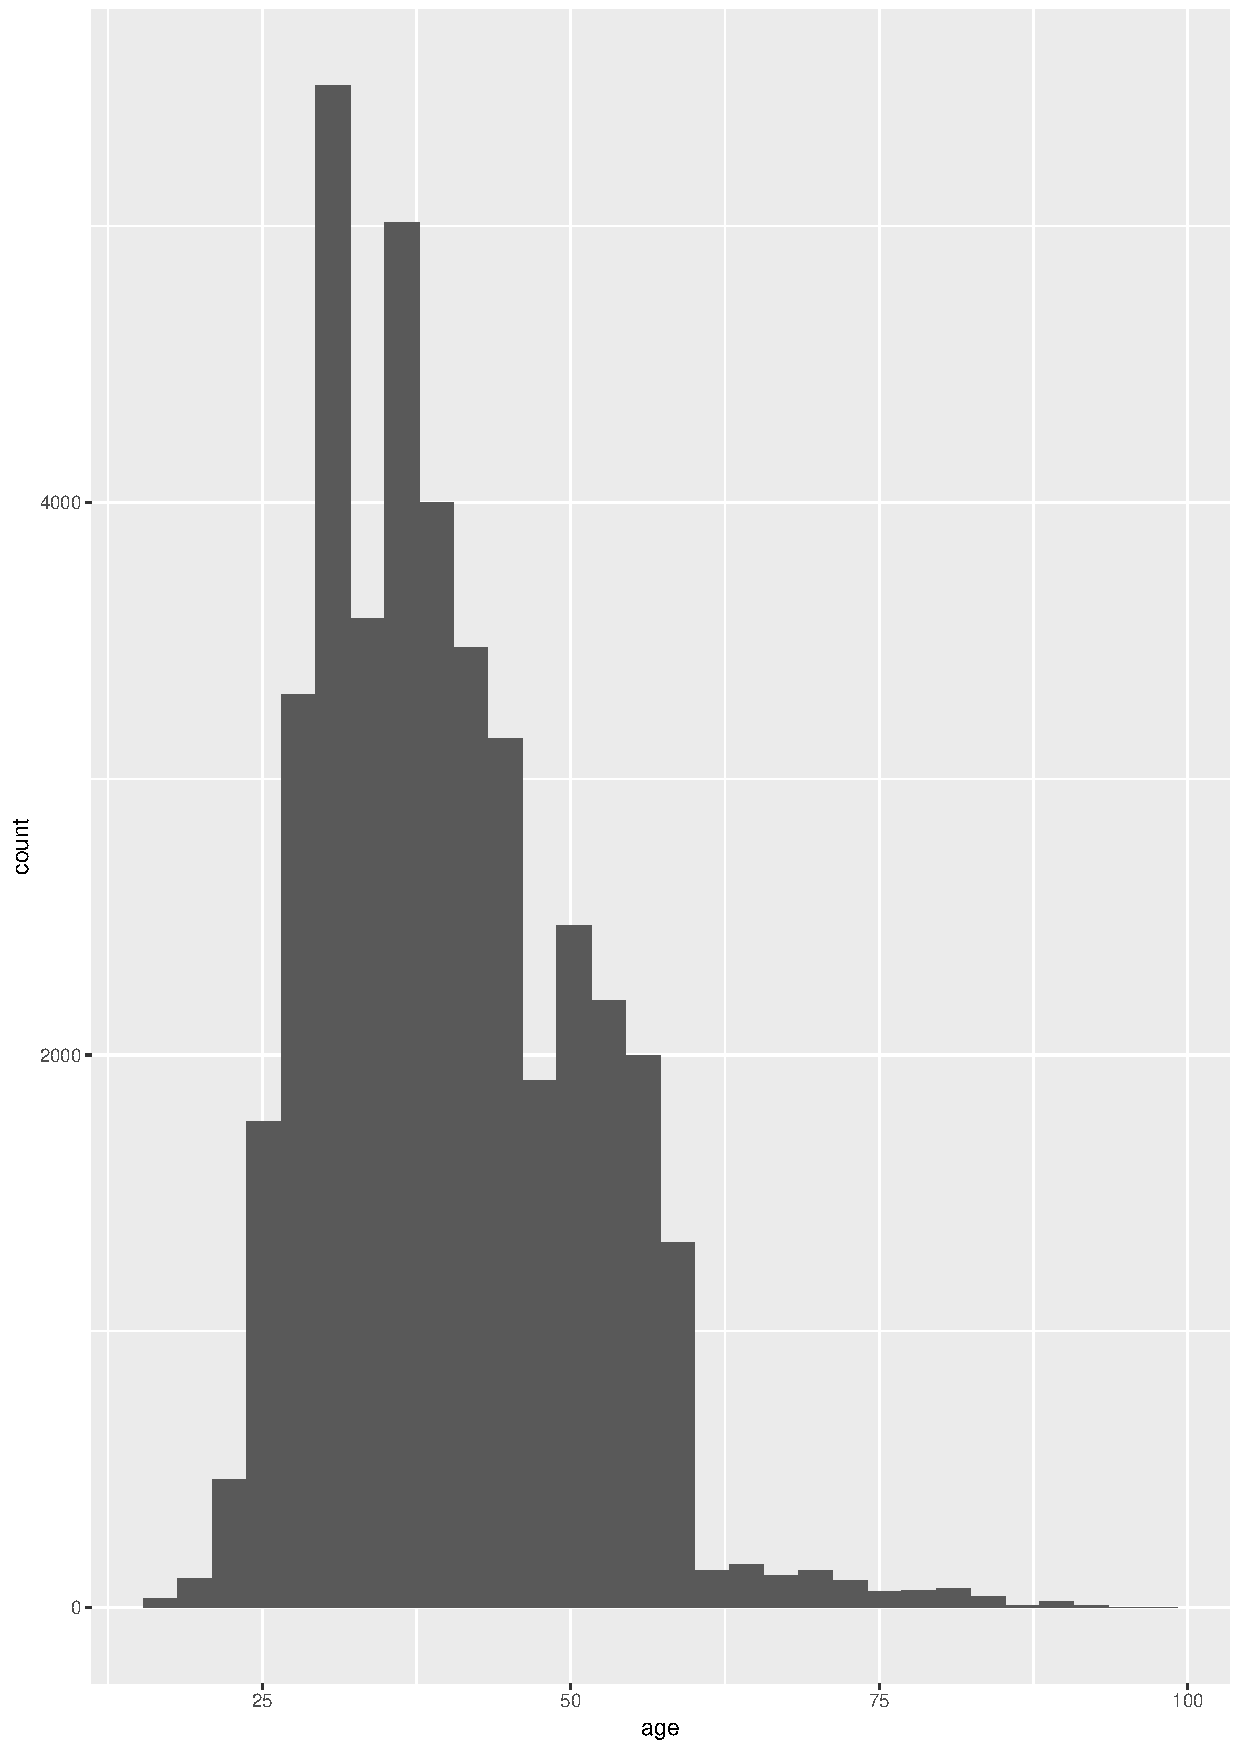
\includegraphics[width=0.7\linewidth]{../MLFBM/MLDATAPRE/Plot1}
	\caption{age distribution}
	\label{fig:plot1}
\end{figure}

\begin{figure}
	\centering
	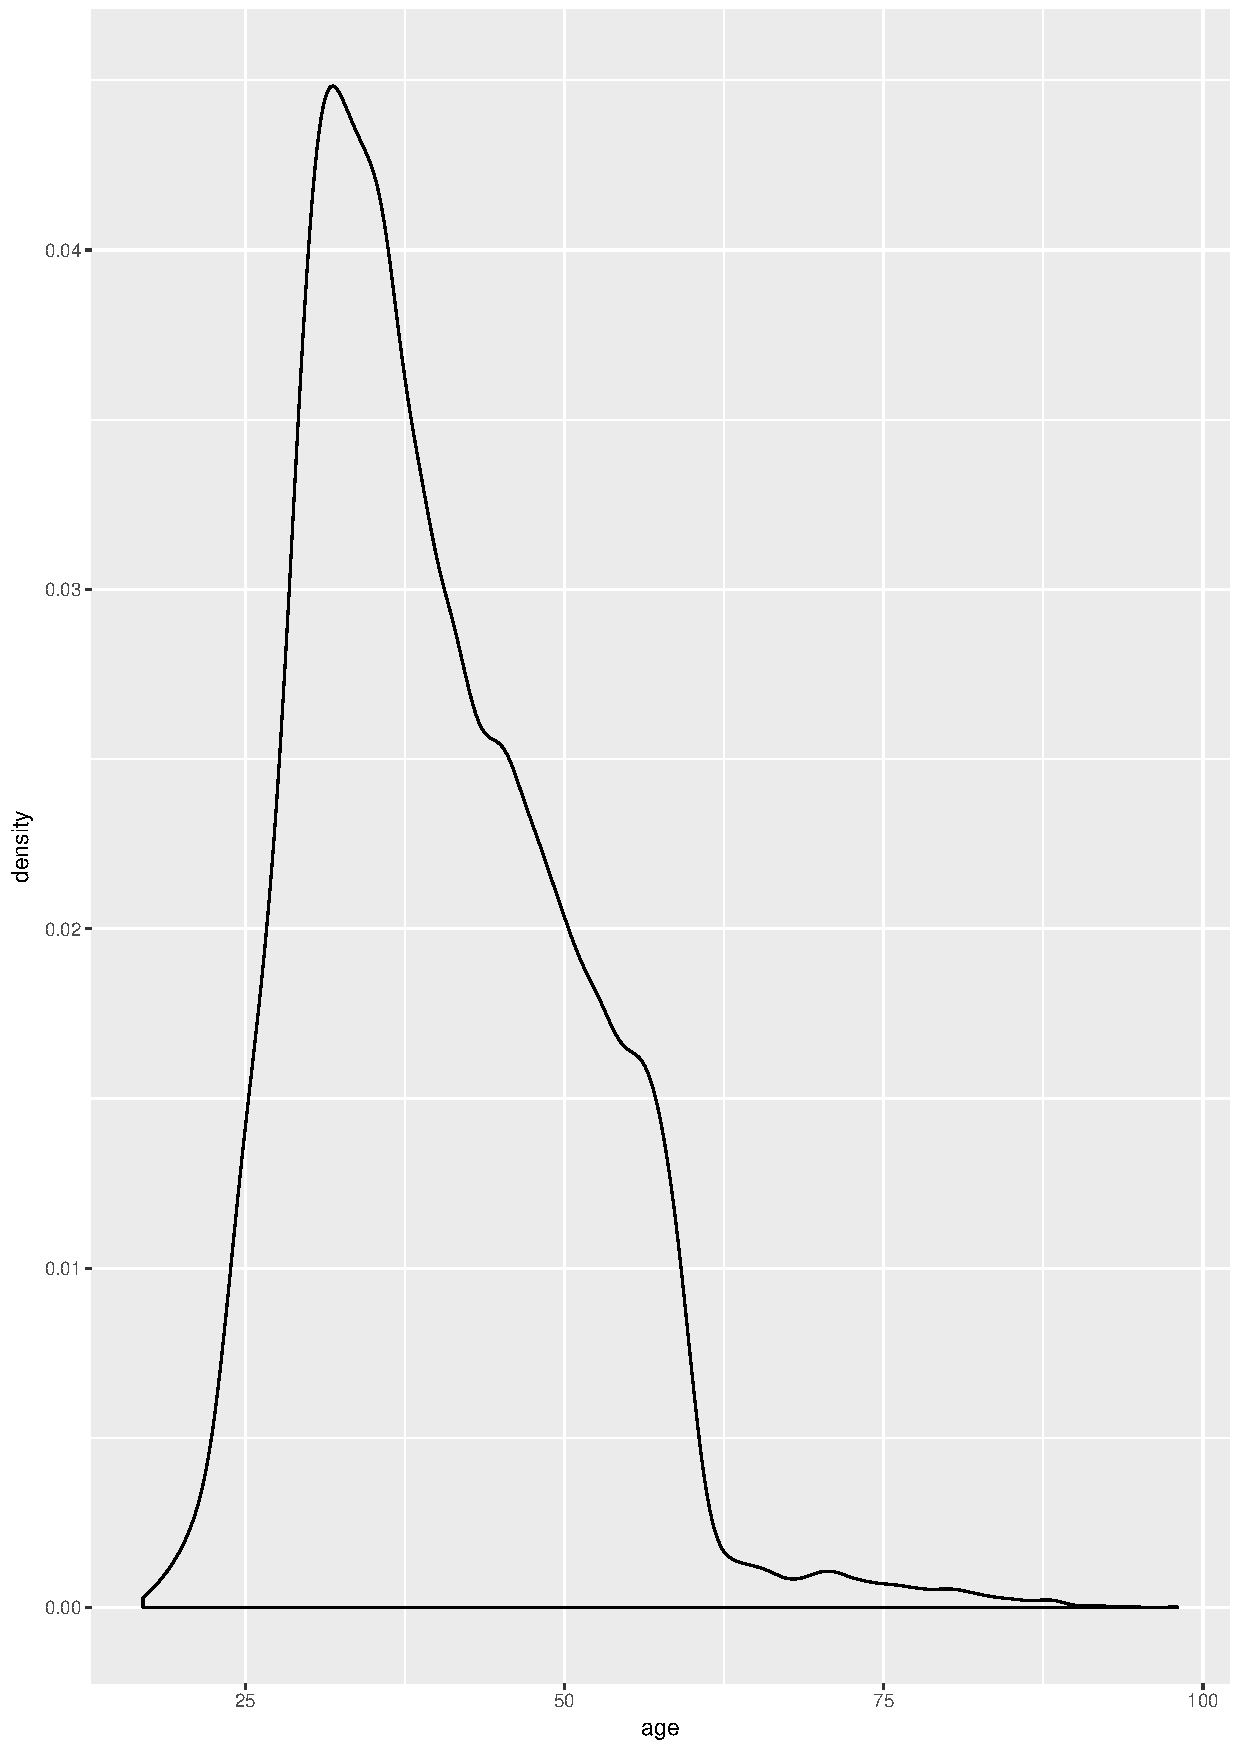
\includegraphics[width=0.7\linewidth]{../MLFBM/MLDATAPRE/Plot2}
	\caption{age density}
	\label{fig:plot2}
\end{figure}

\begin{figure}
	\centering
	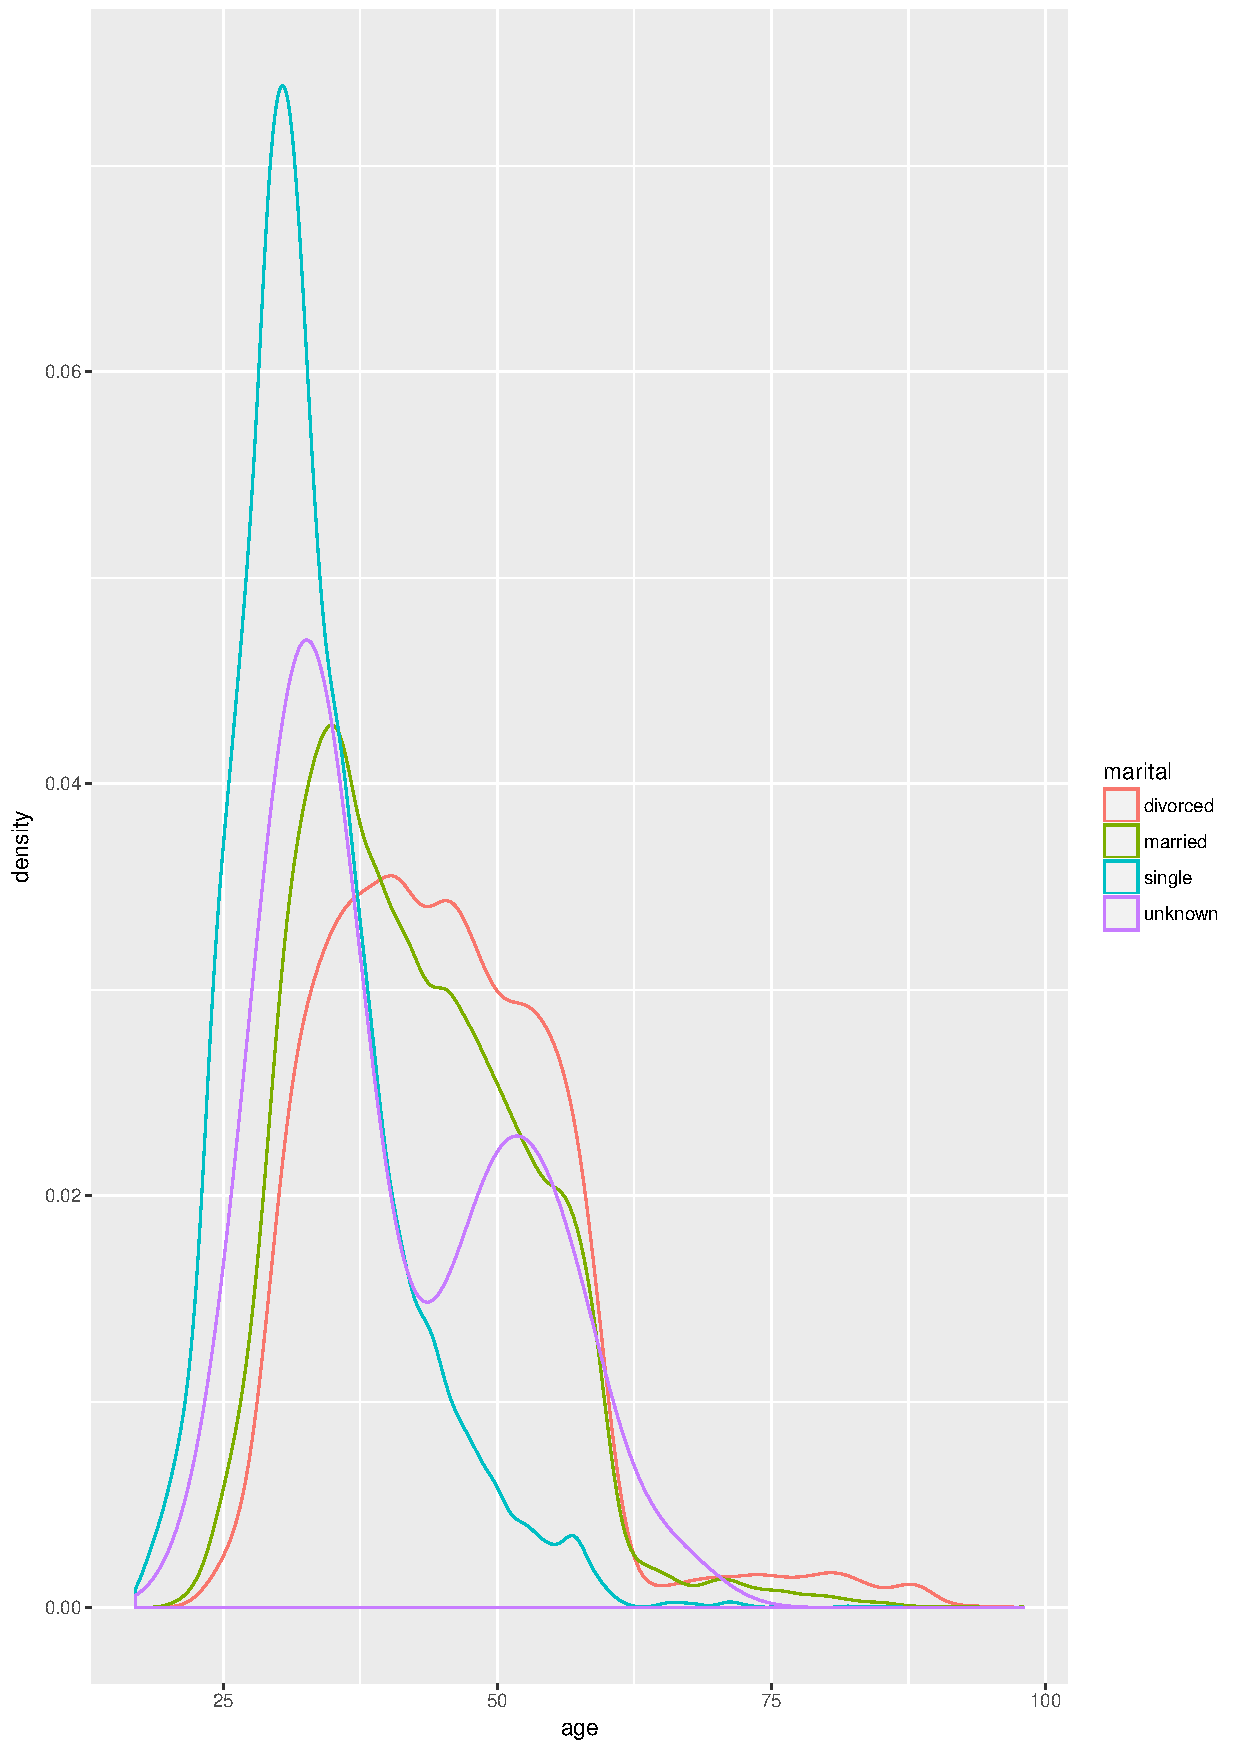
\includegraphics[width=0.7\linewidth]{../MLFBM/MLDATAPRE/Plot3}
	\caption{age-marital}
	\label{fig:plot3}
\end{figure}

\begin{figure}
	\centering
	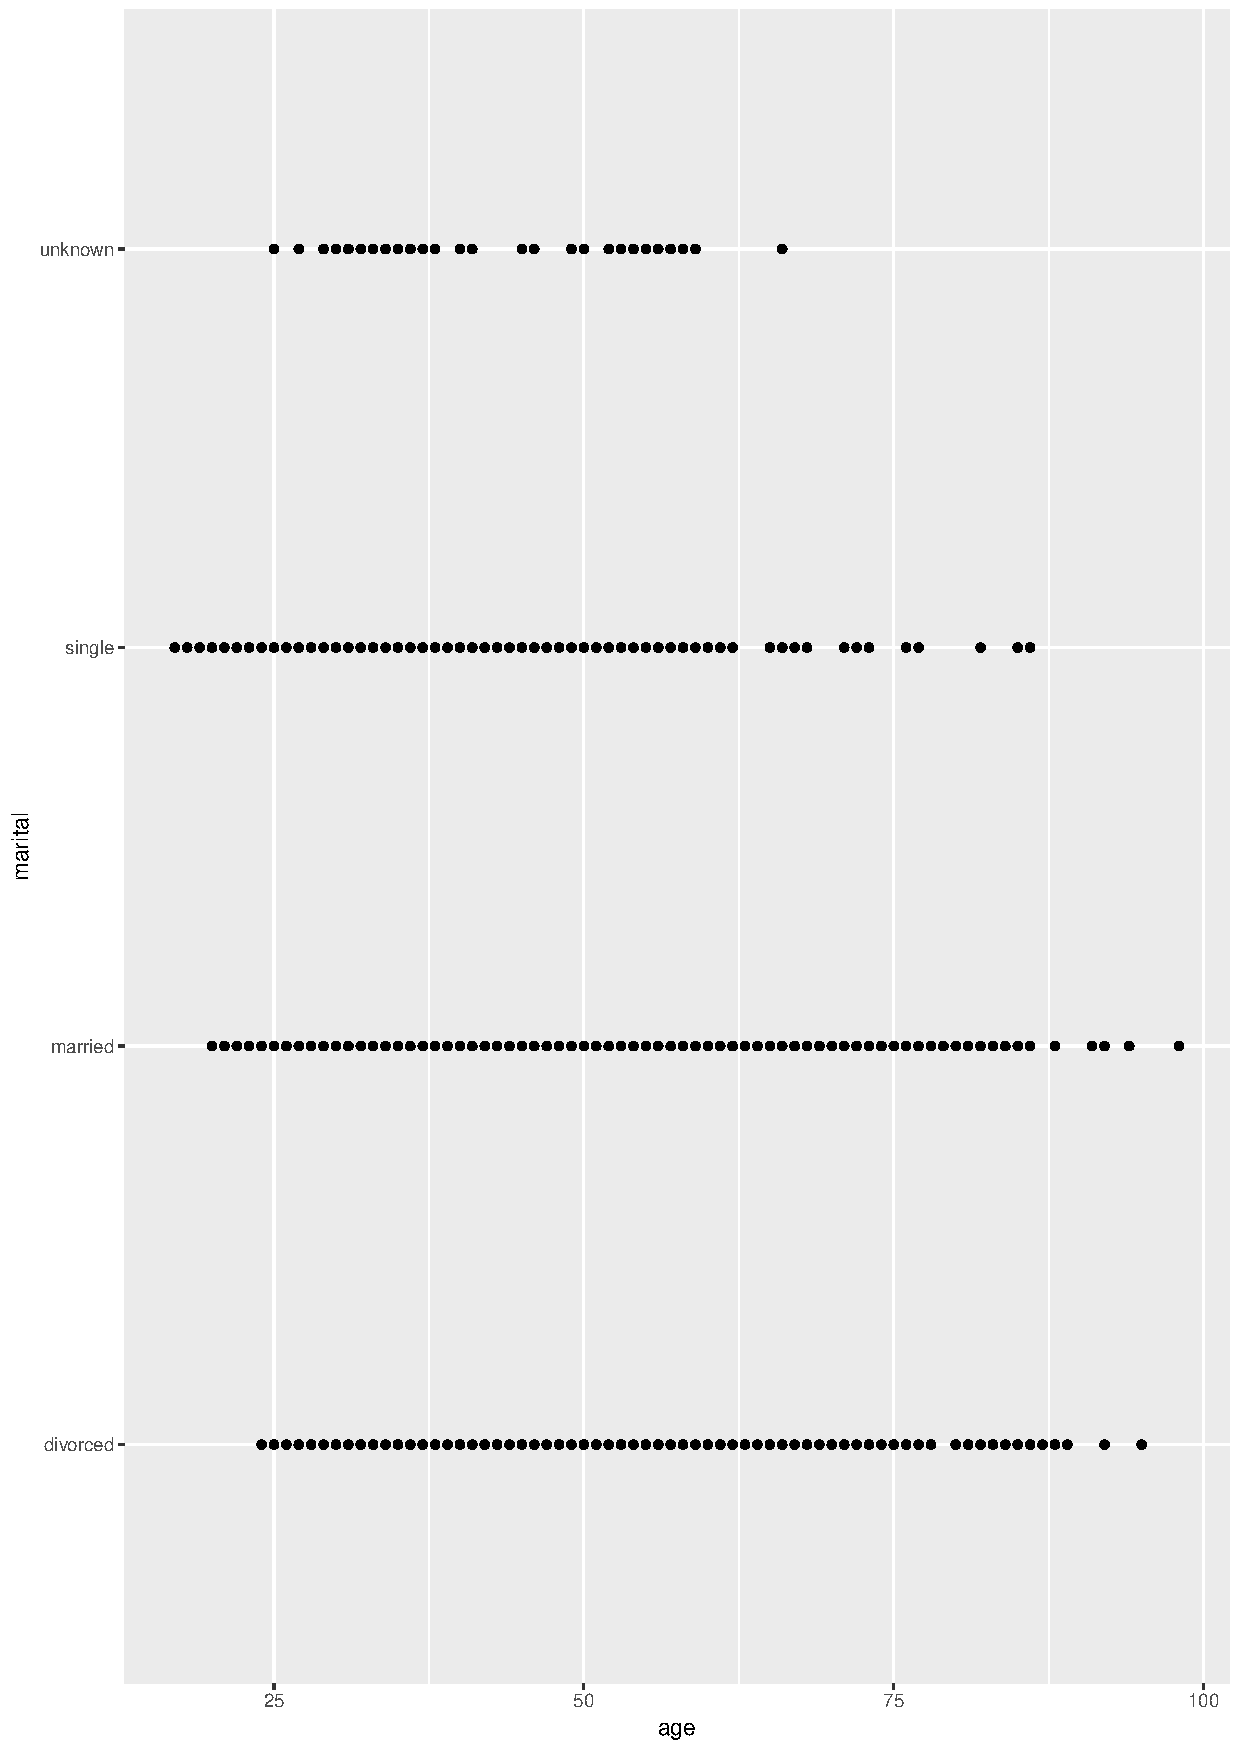
\includegraphics[width=0.7\linewidth]{../MLFBM/MLDATAPRE/Plot4}
	\caption{age-marital density}
	\label{fig:plot4}
\end{figure}

\begin{figure}
	\centering
	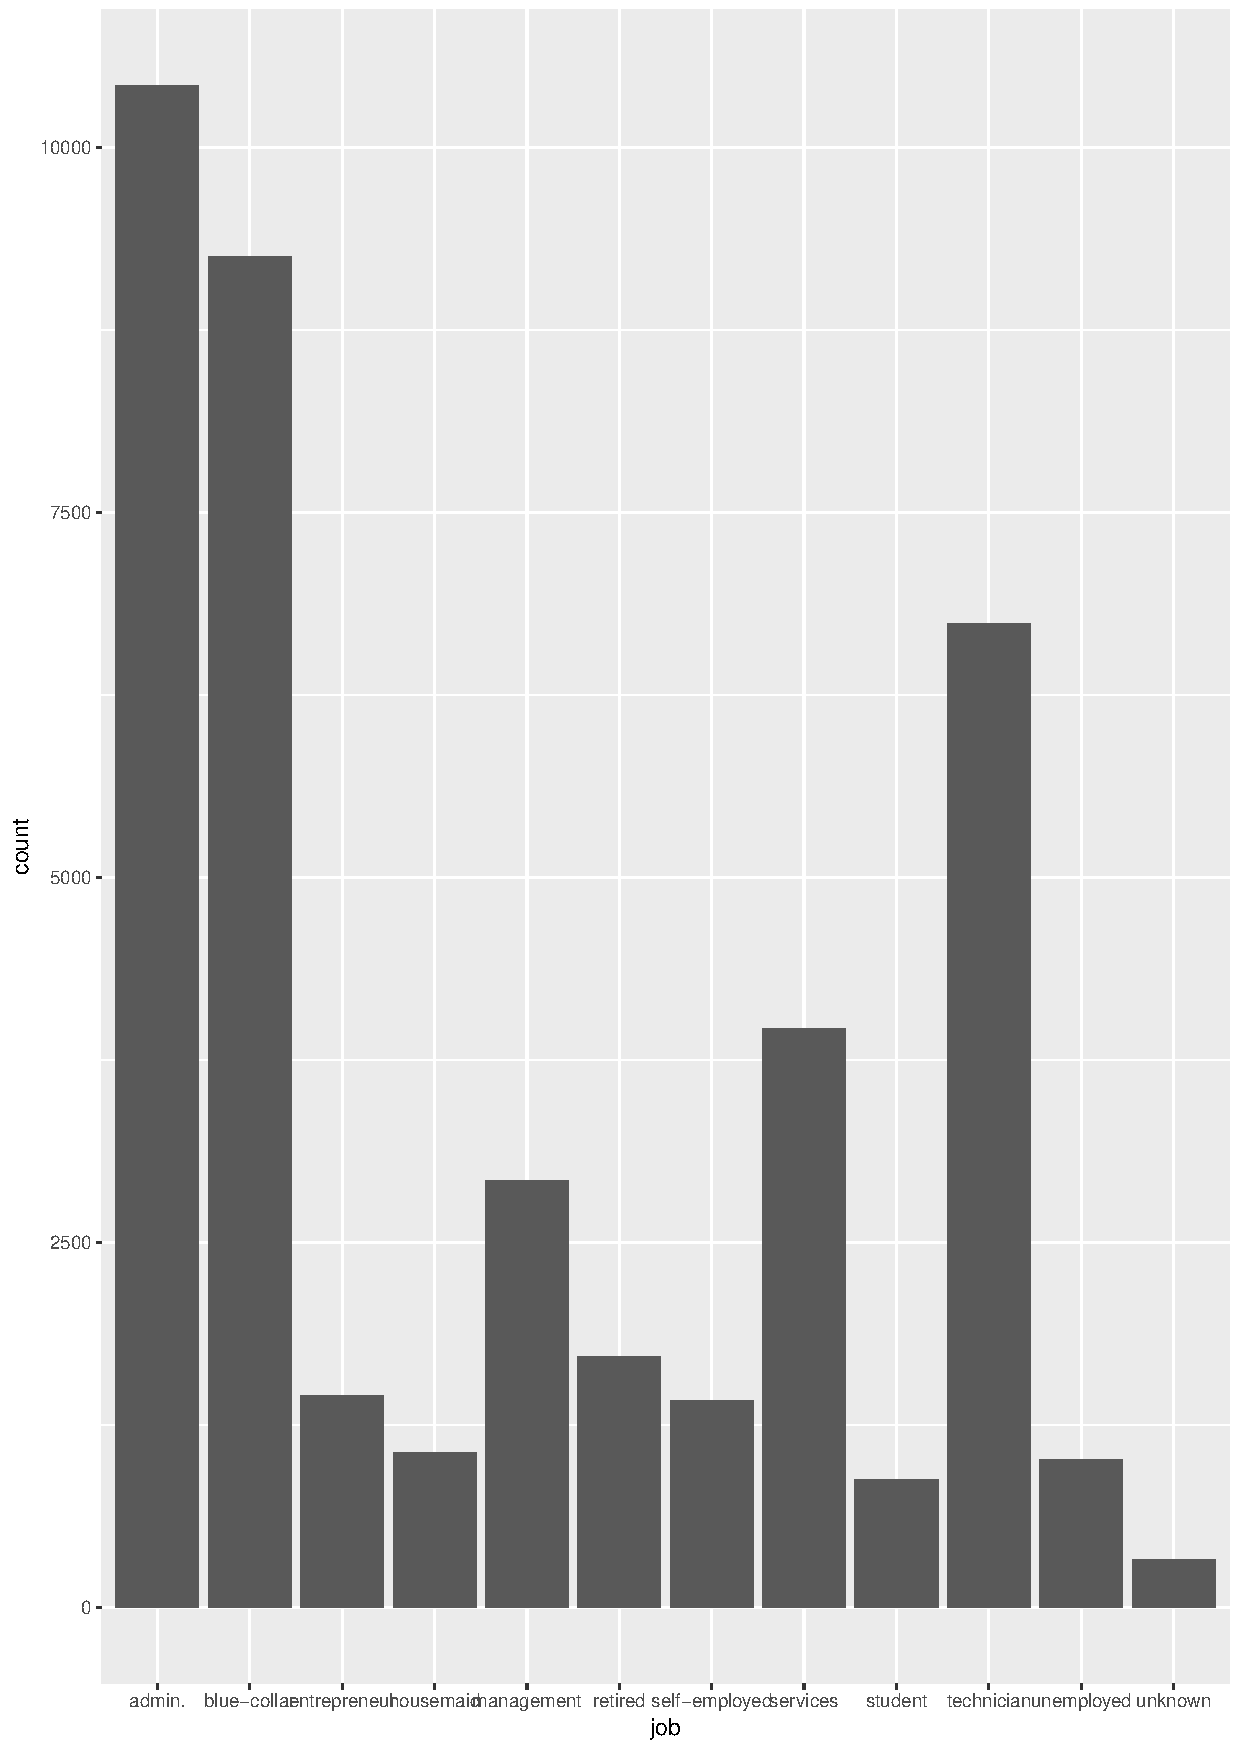
\includegraphics[width=0.7\linewidth]{../MLFBM/MLDATAPRE/Plot5}
	\caption{job distribution}
	\label{fig:plot5}
\end{figure}

\begin{figure}
	\centering
	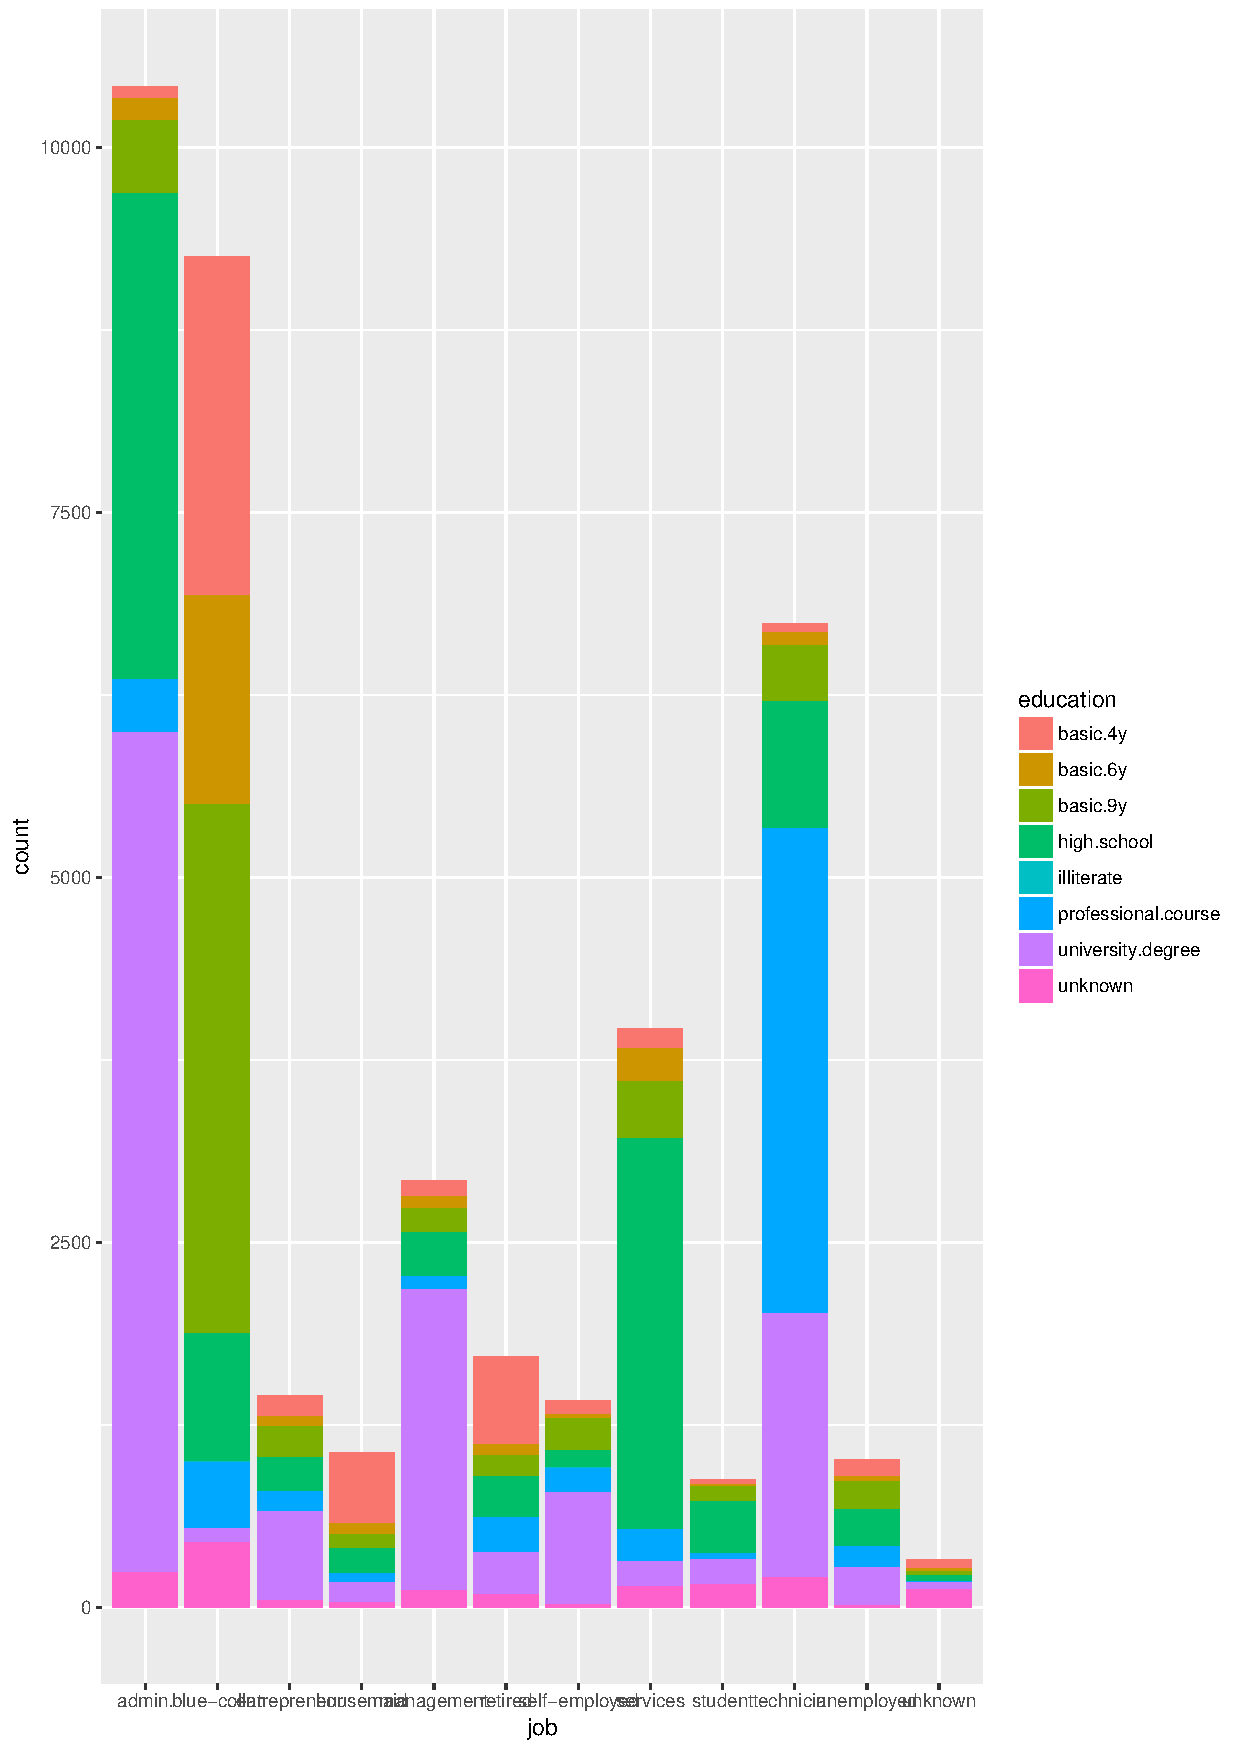
\includegraphics[width=0.7\linewidth]{../MLFBM/MLDATAPRE/Plot6}
	\caption{job-education distribution}
	\label{fig:plot6}
\end{figure}

\begin{figure}
	\centering
	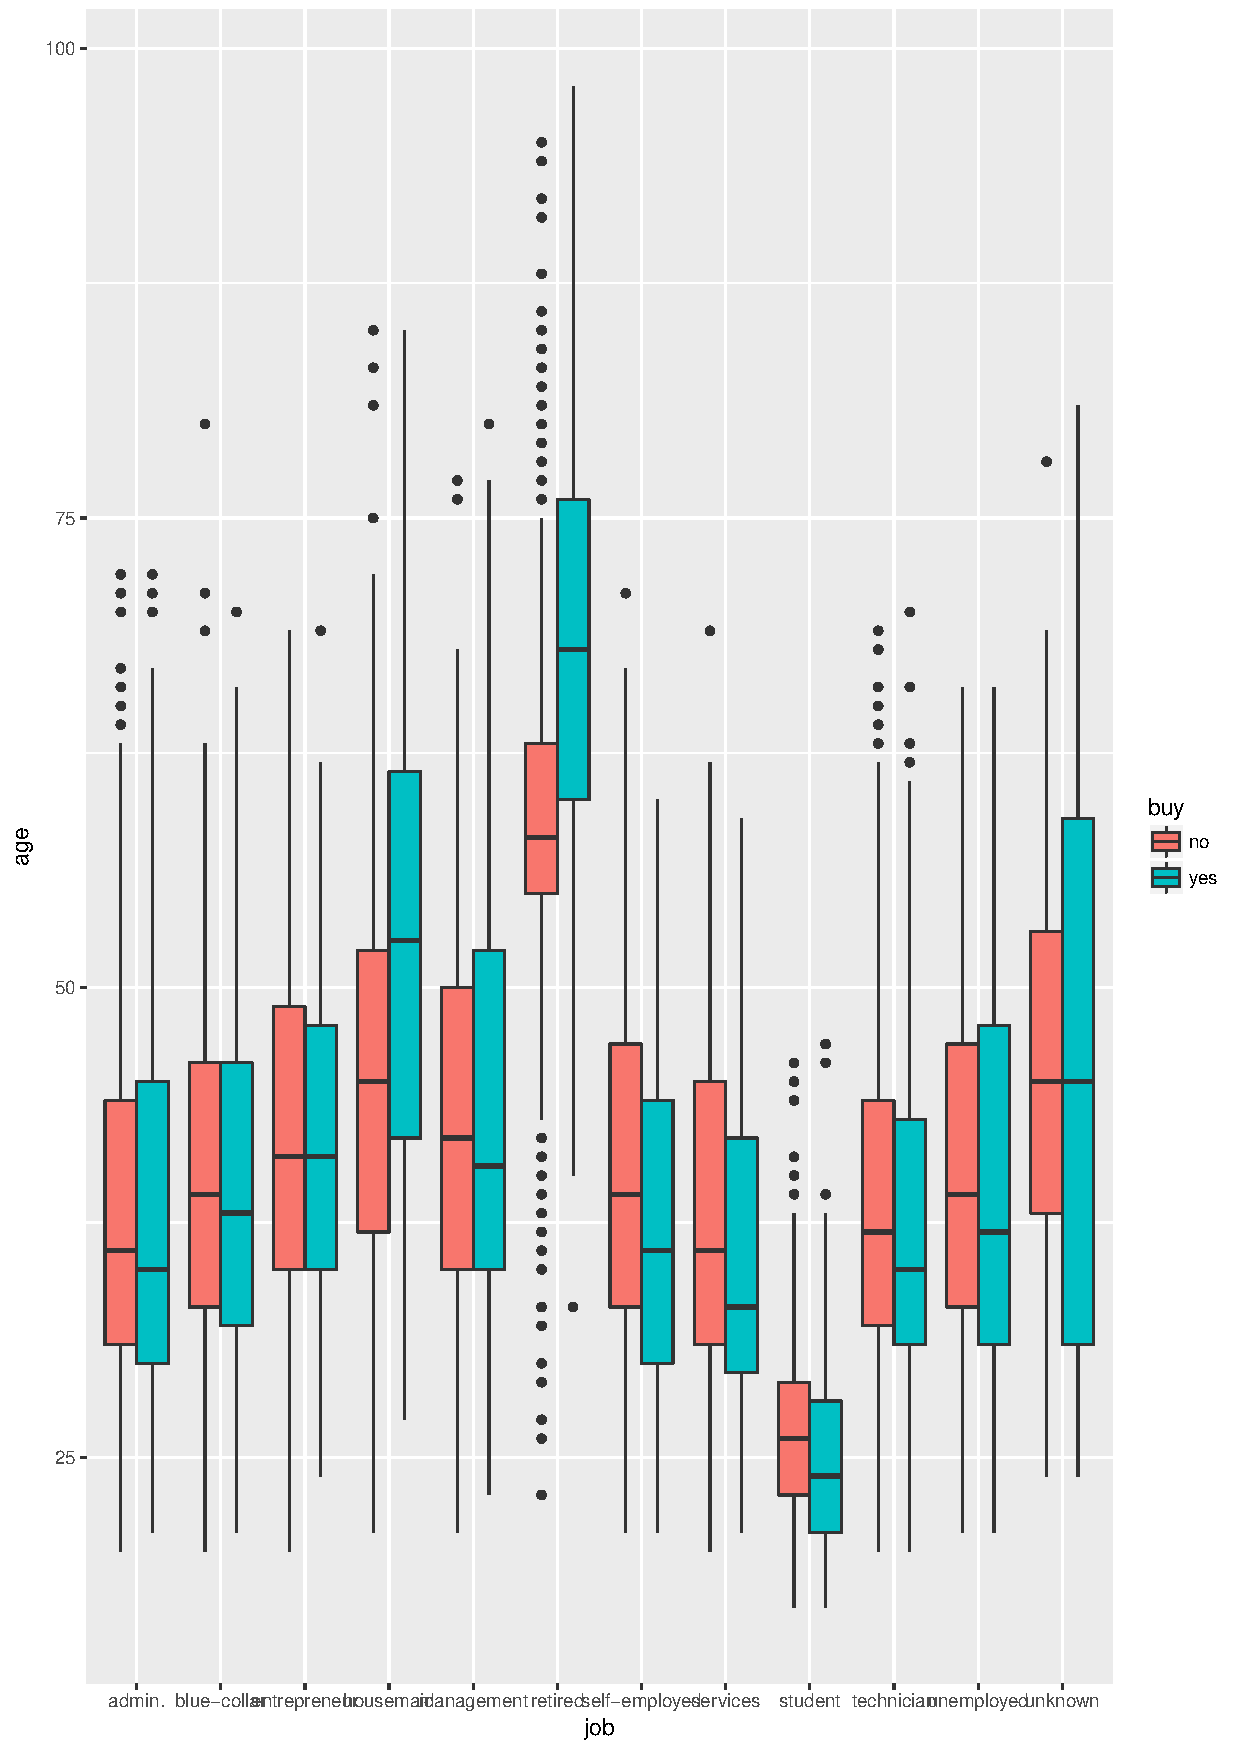
\includegraphics[width=0.7\linewidth]{../MLFBM/MLDATAPRE/Plot7}
	\caption{Job-age buy decision}
	\label{fig:plot7}
\end{figure}

\begin{figure}
	\centering
	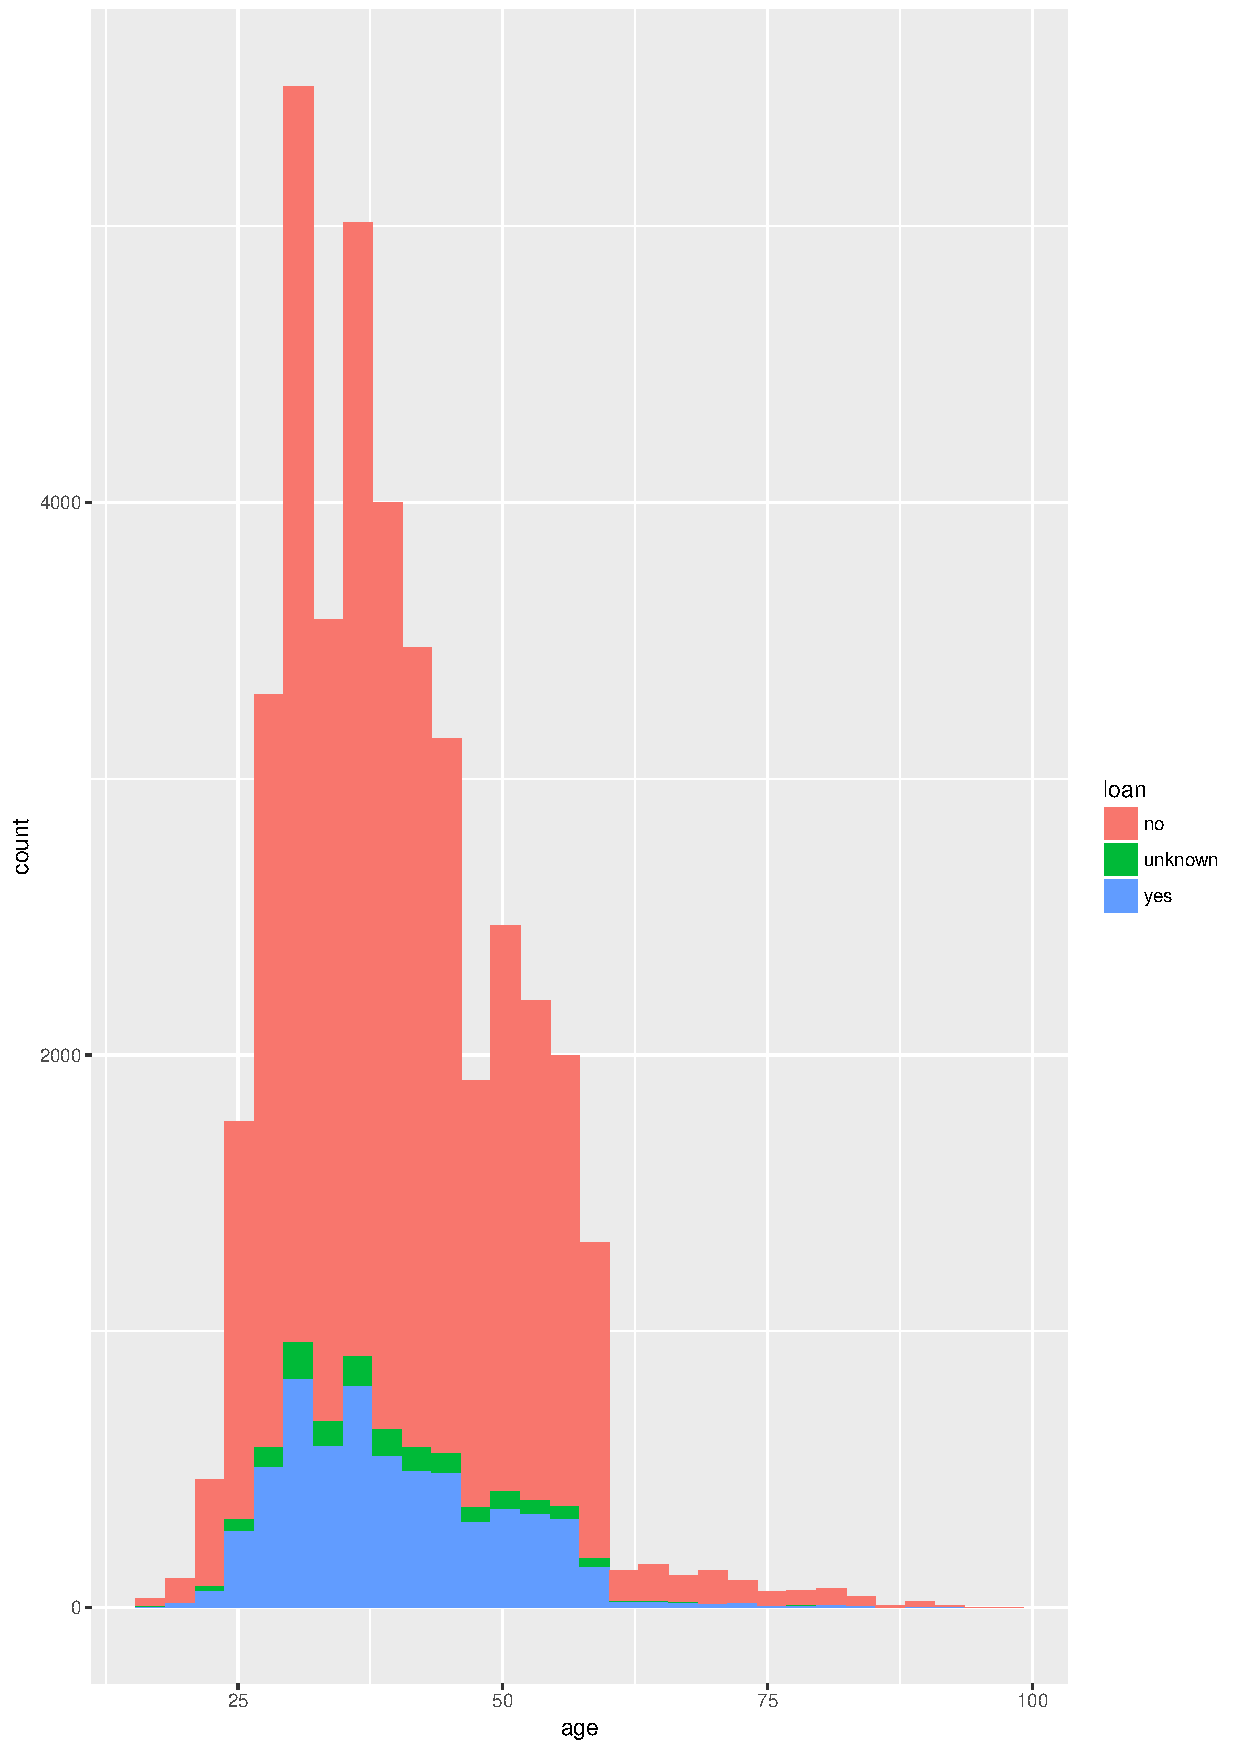
\includegraphics[width=0.7\linewidth]{../MLFBM/MLDATAPRE/Plot8}
	\caption{age-loan distribution}
	\label{fig:plot8}
\end{figure}

\begin{figure}
	\centering
	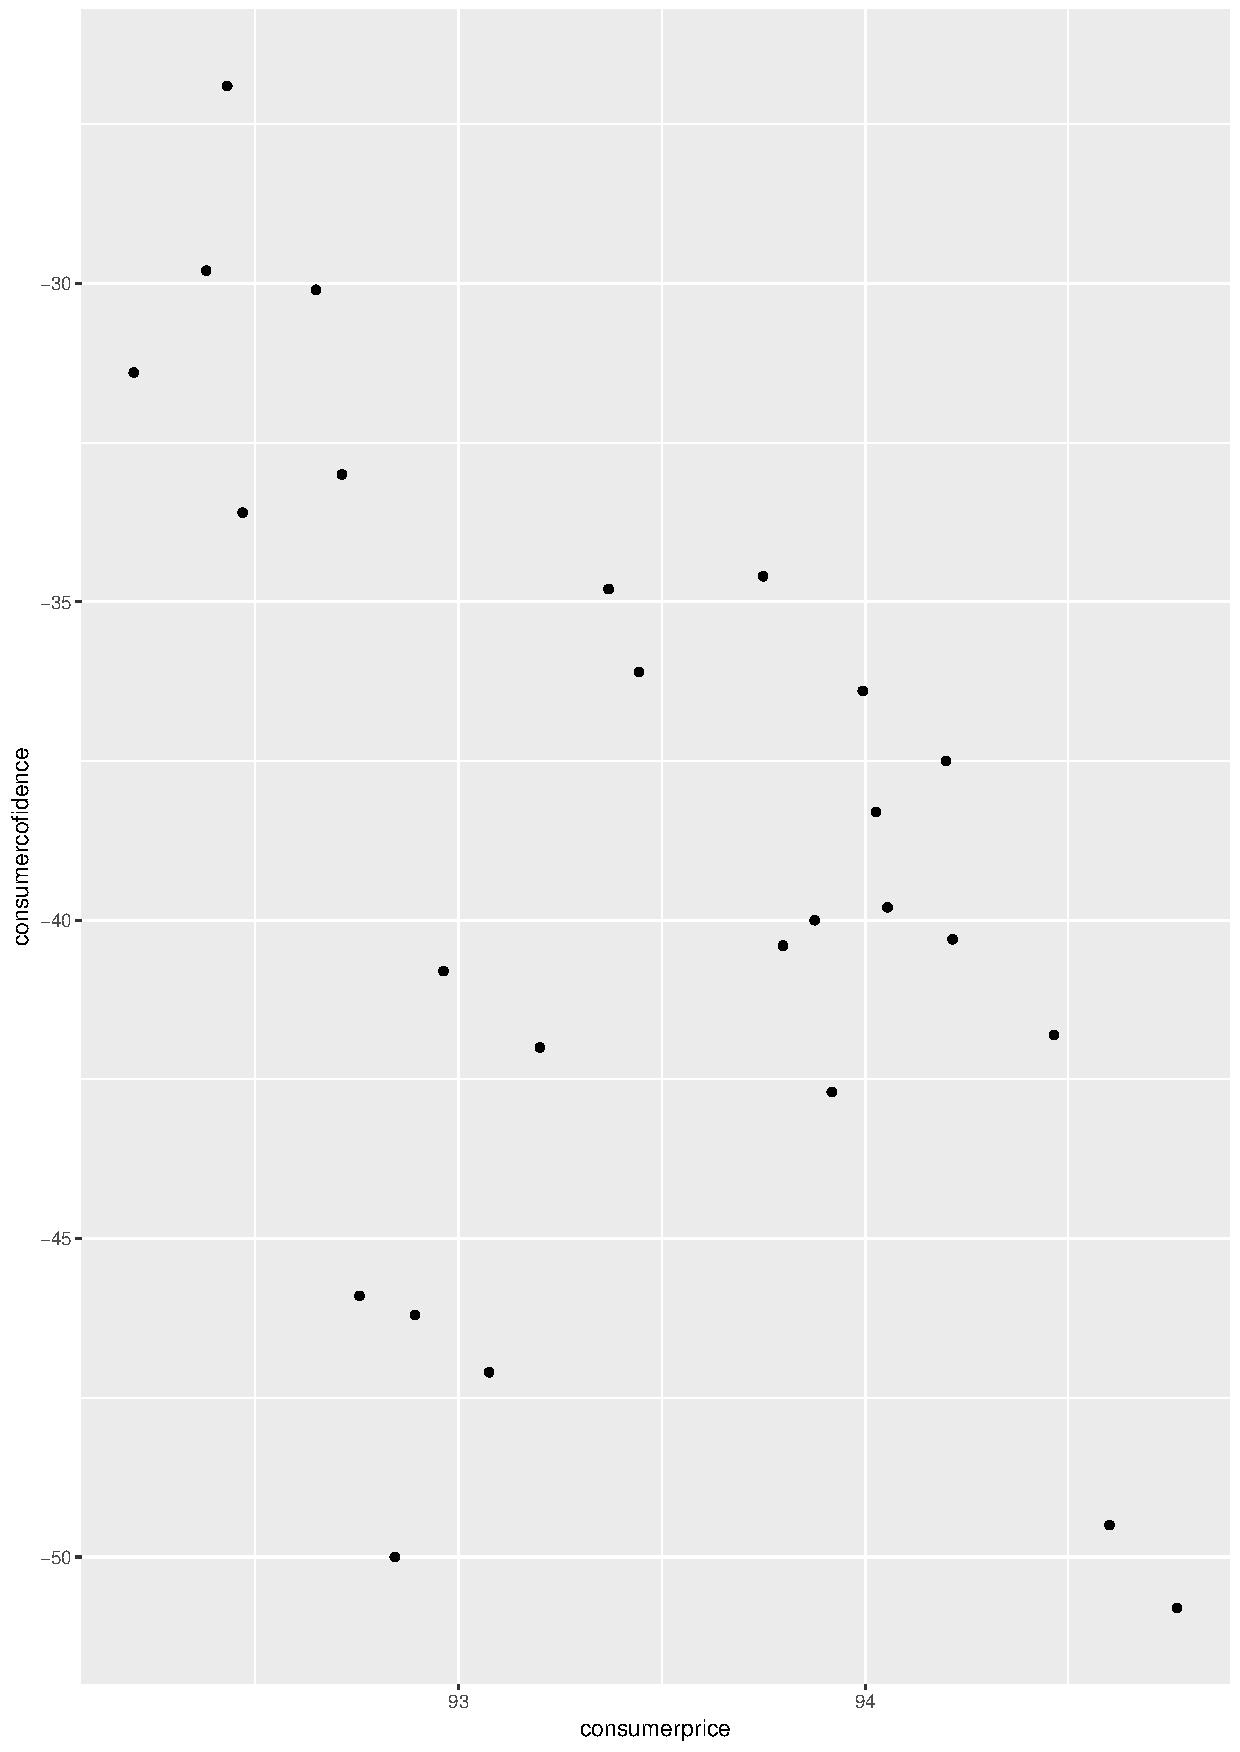
\includegraphics[width=0.7\linewidth]{../MLFBM/MLDATAPRE/Plot9}
	\caption{scatter diagram:consumer price vs consumer confidence}
	\label{fig:plot9}
\end{figure}
\begin{figure}
	\centering
	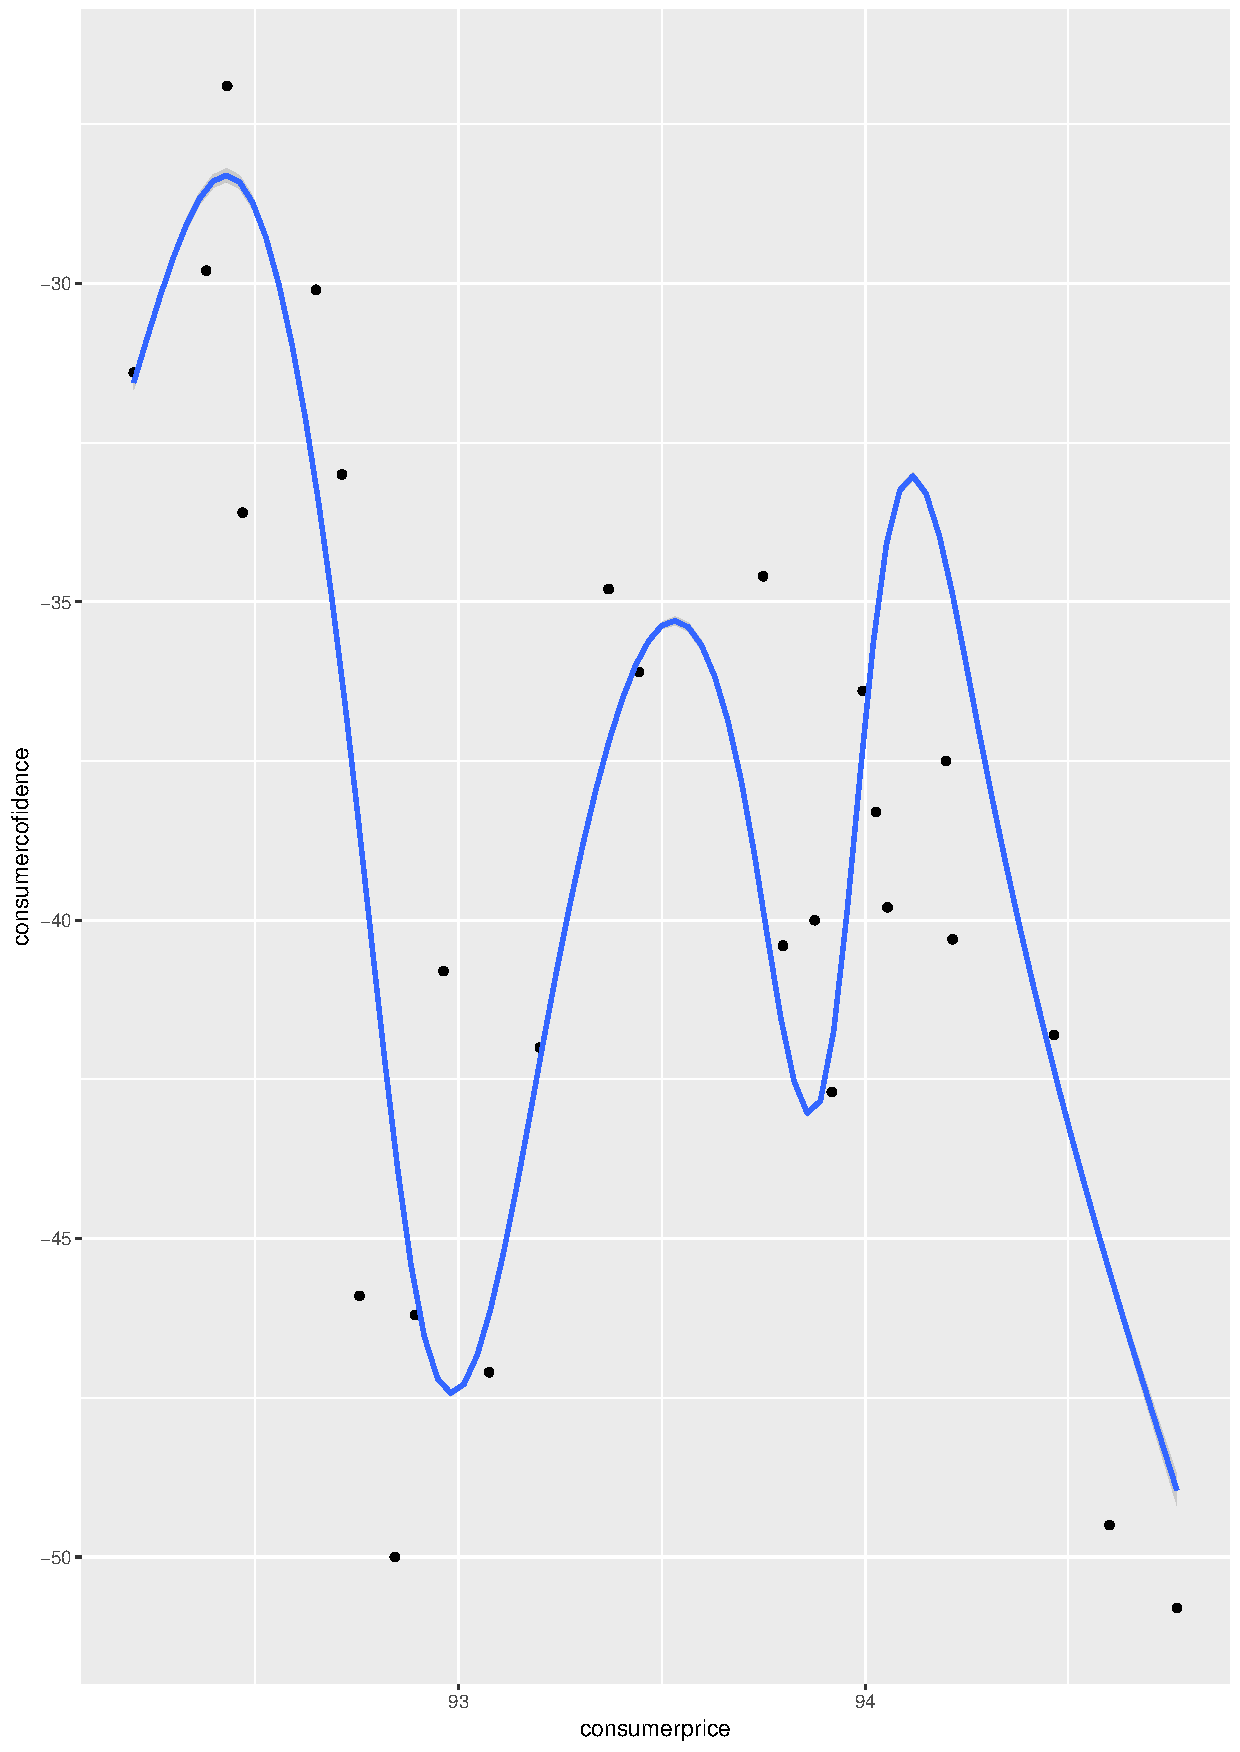
\includegraphics[width=0.7\linewidth]{../MLFBM/MLDATAPRE/Plot10}
	\caption{scatter diagram with trend:consumer price vs consumer confidence}
	\label{fig:plot10}
\end{figure}

\begin{figure}
	\centering
	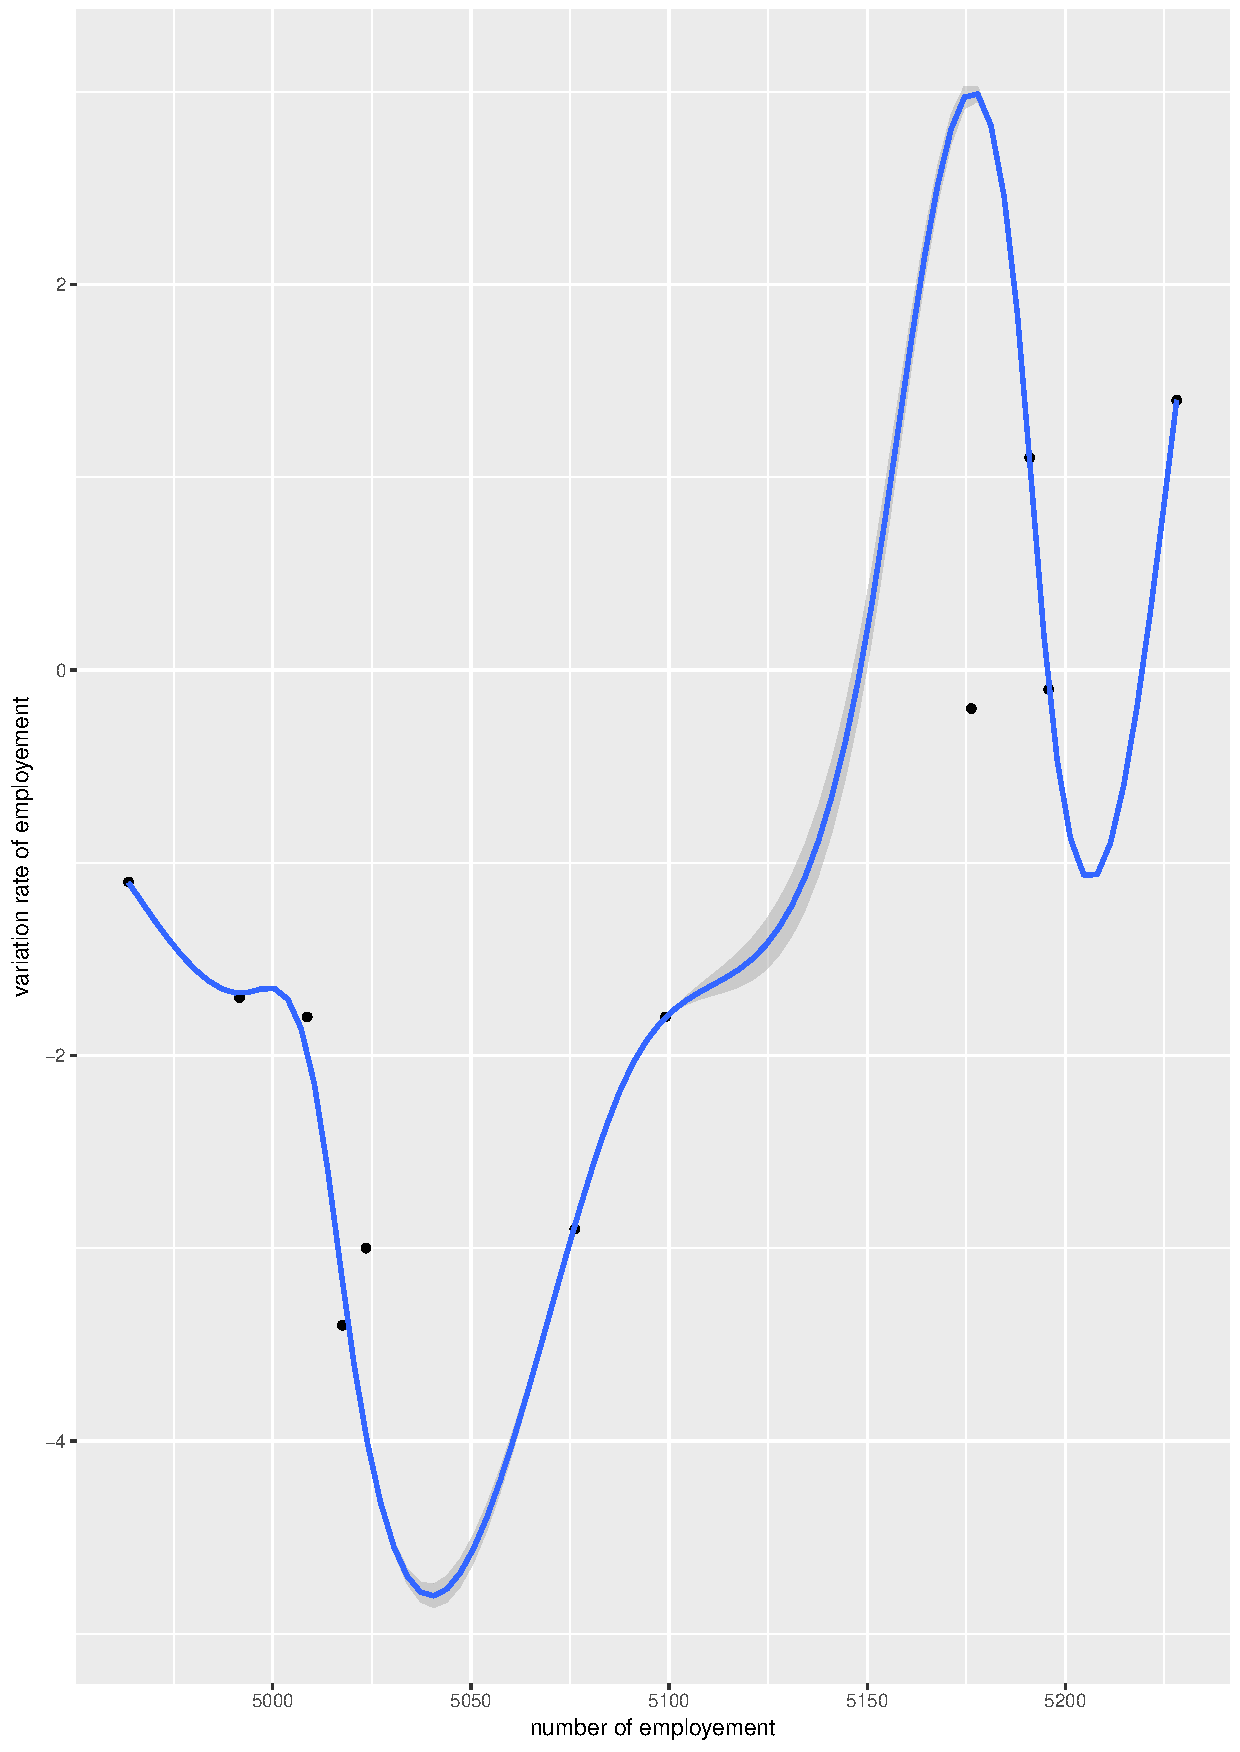
\includegraphics[width=0.7\linewidth]{../MLFBM/MLDATAPRE/Plot11}
	\caption{scatter diagram with trend:number of employement vs employment variation rate}
	\label{fig:plot11}
\end{figure}


%{Data Completion}


%{Logistic Regression}
\begin{figure}
	\centering
	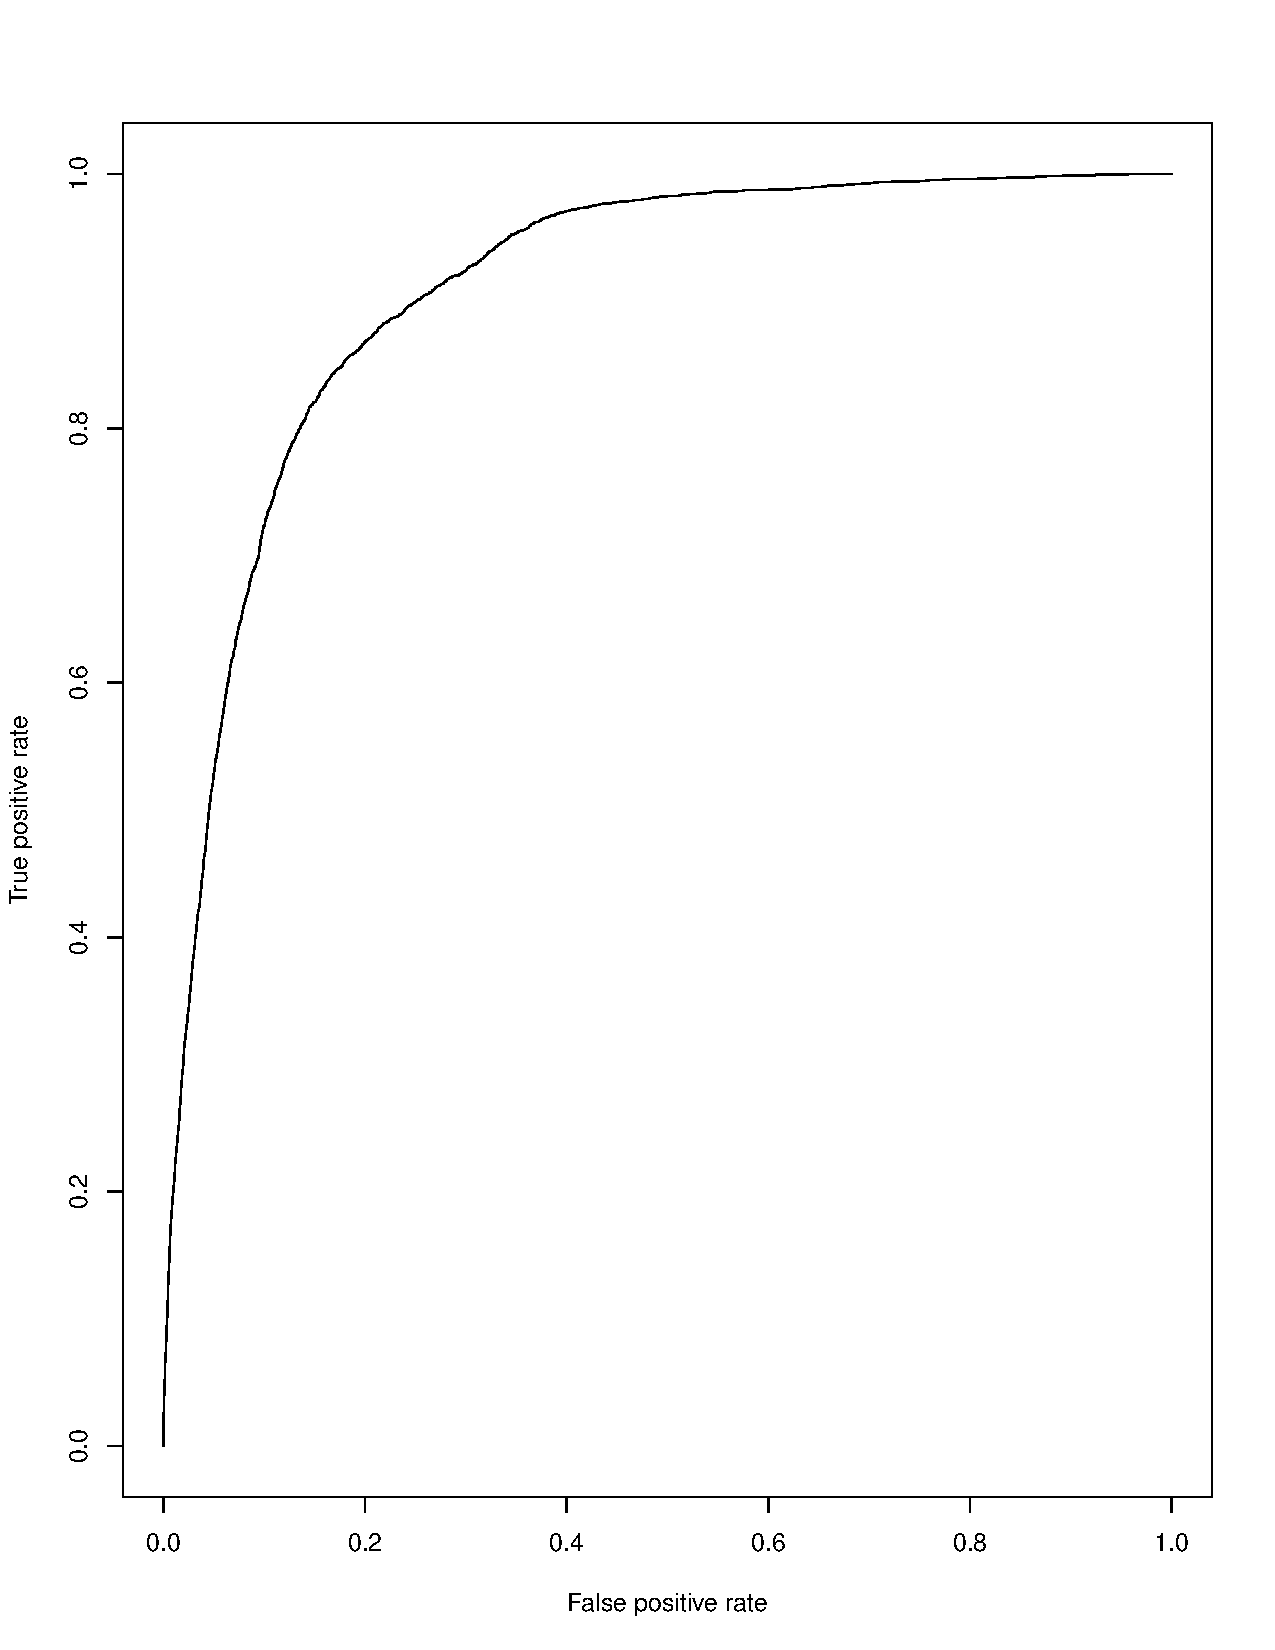
\includegraphics[width=0.7\linewidth]{../MLFBM/logisticregression/ROC_lr}
	\caption{ROC of Logistic Regression}
	\label{fig:roclr}
\end{figure}

%{Decision Tree}

\begin{figure}
	\centering
	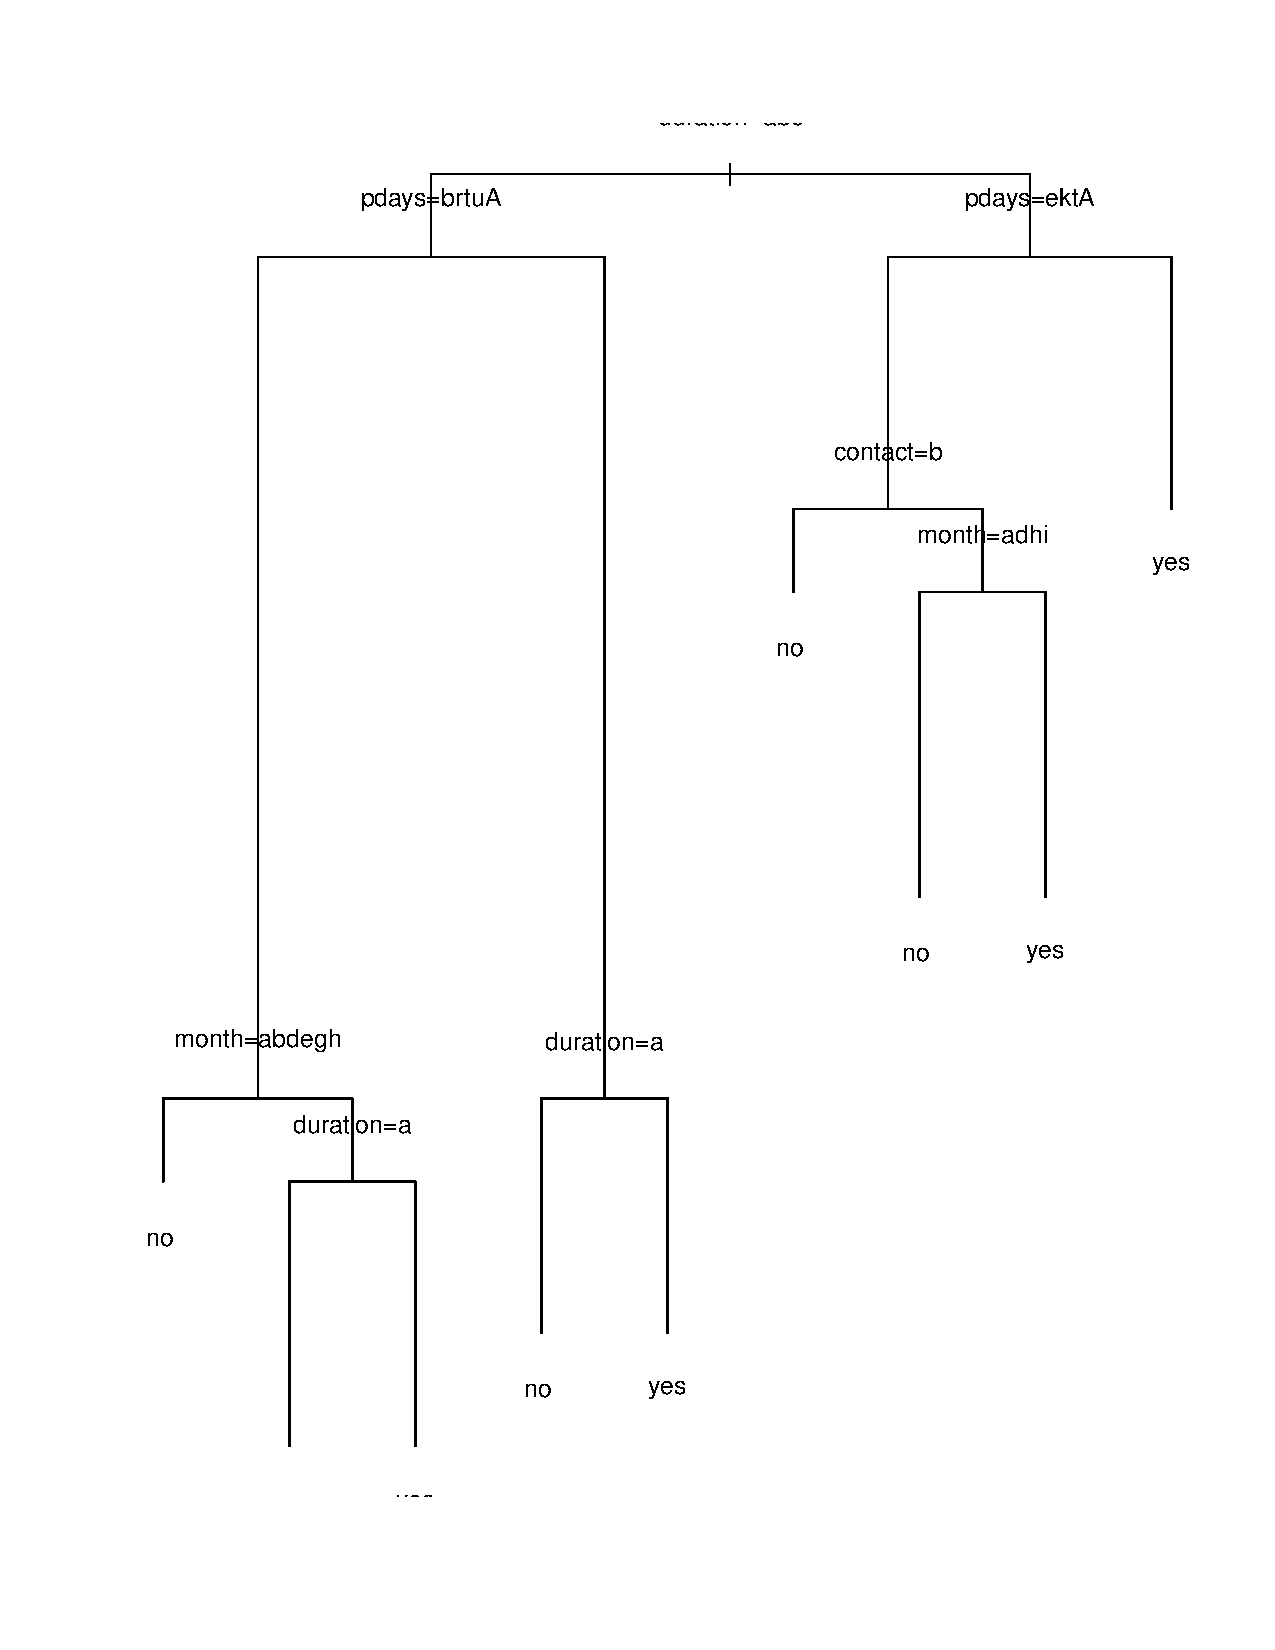
\includegraphics[width=0.7\linewidth]{../MLFBM/decisiontree/plot_dt}
	\caption{Plot Decision Tree}
	\label{fig:plotdt}
\end{figure}

\begin{figure}
	\centering
	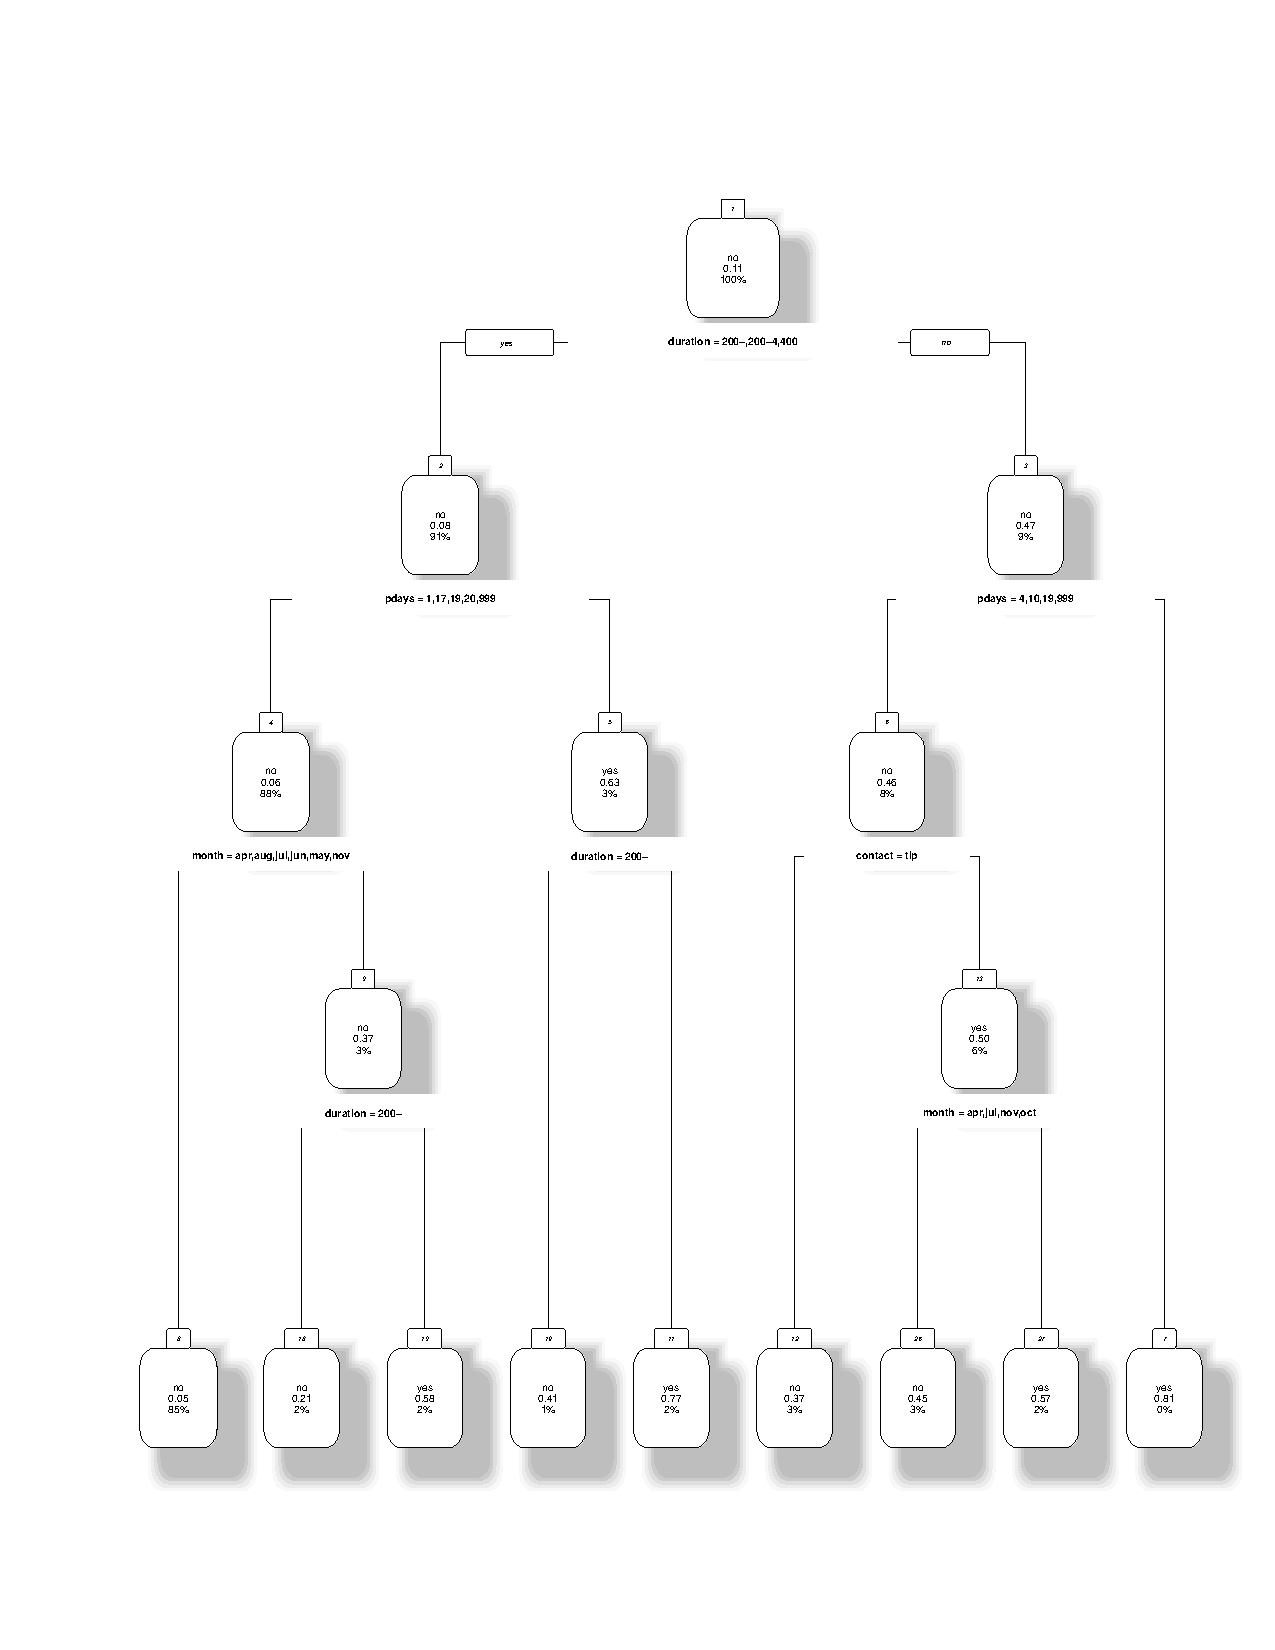
\includegraphics[width=0.7\linewidth]{../MLFBM/decisiontree/prp_dt}
	\caption{Visualize through prp()}
	\label{fig:prpdt}
\end{figure}

\begin{figure}
	\centering
	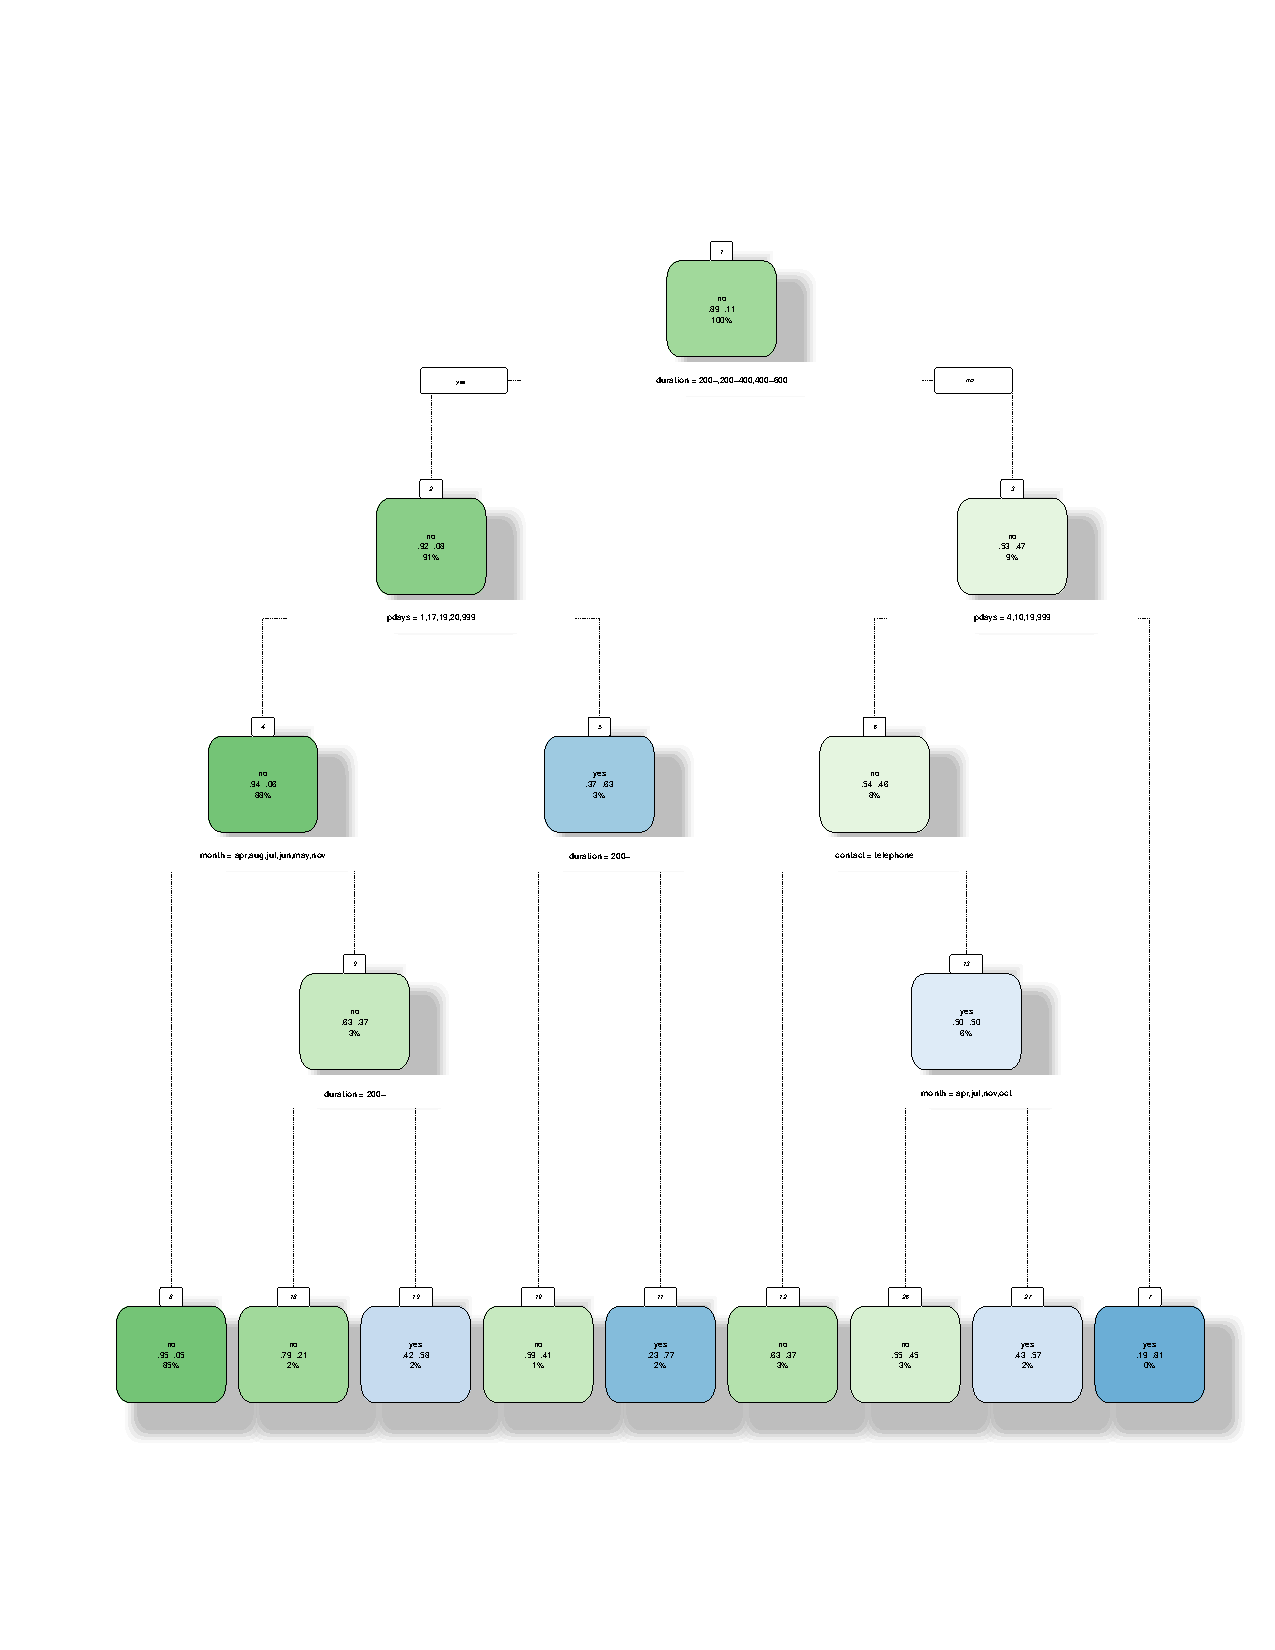
\includegraphics[width=0.7\linewidth]{../MLFBM/decisiontree/part-lot_dt}
	\caption{Visualize through rpart.plot()}
	\label{fig:part-lotdt}
\end{figure}

\begin{figure}
	\centering
	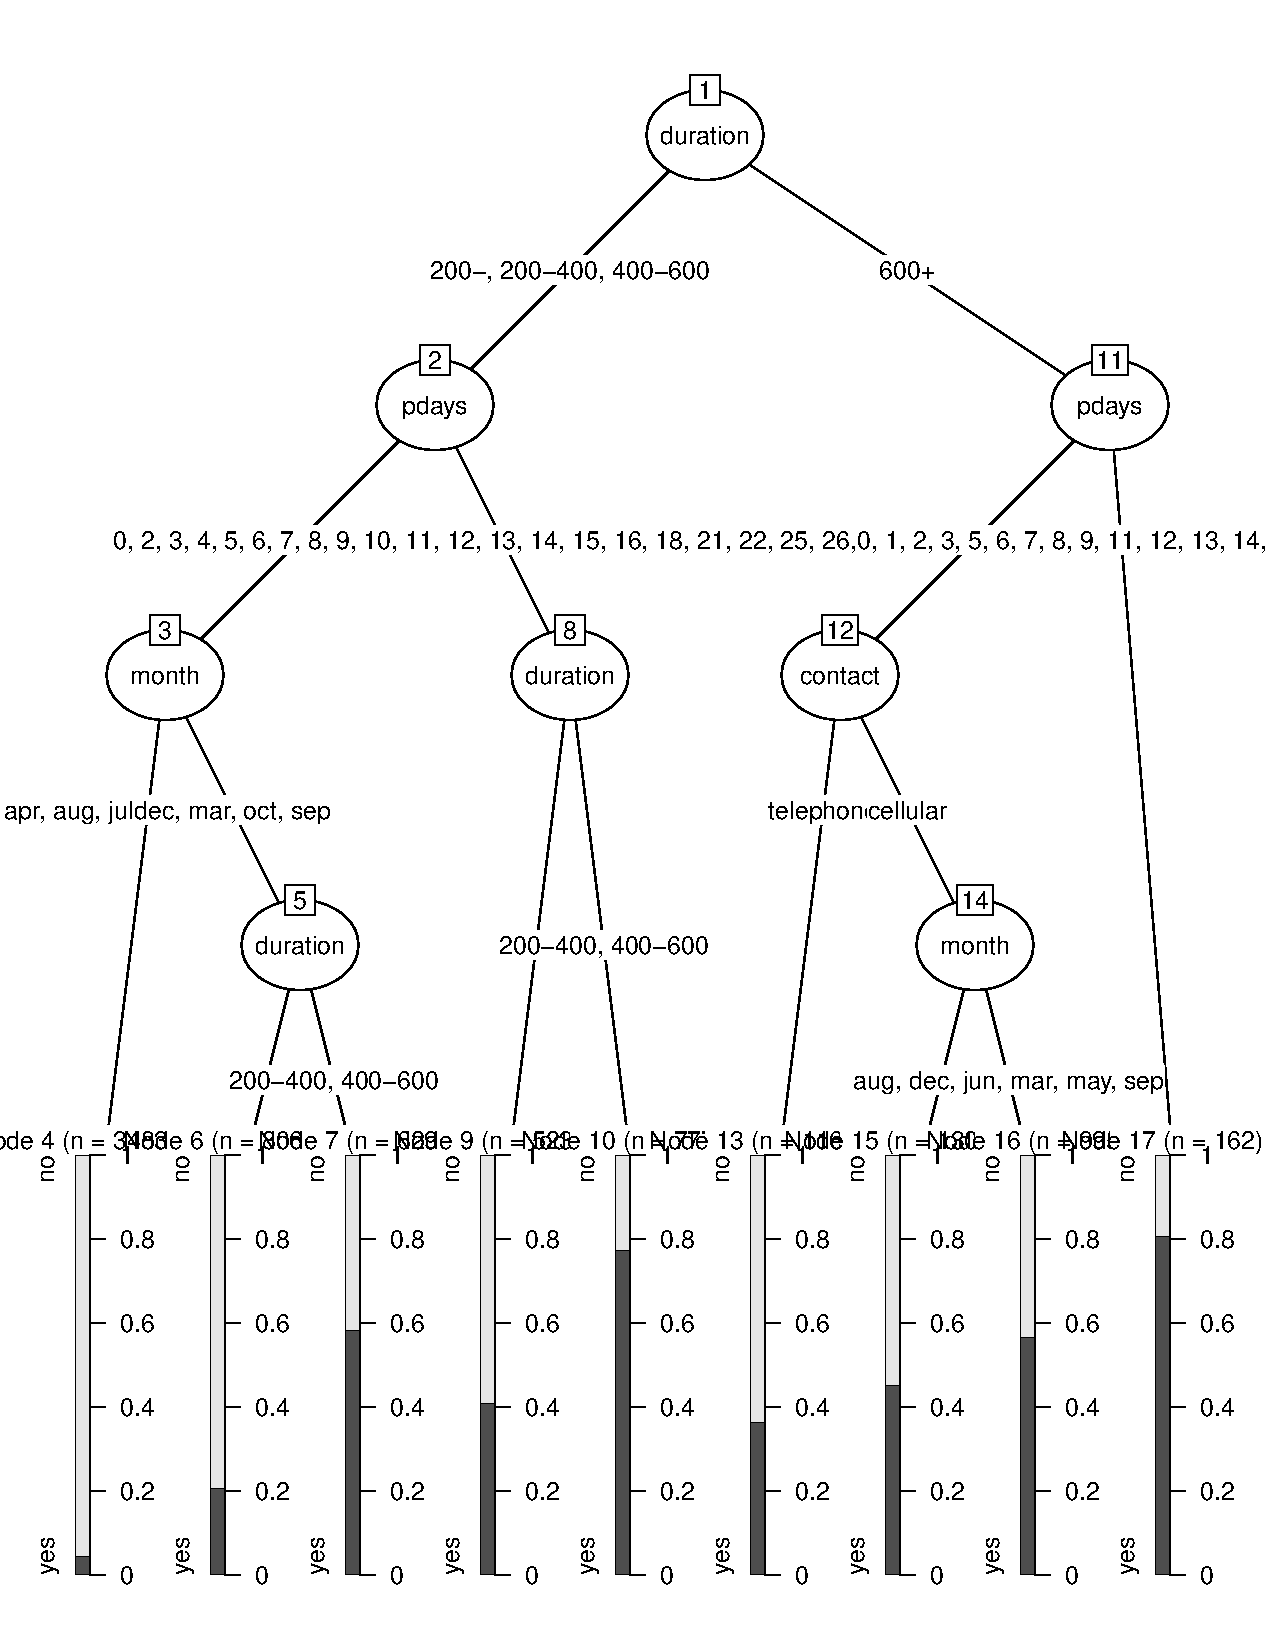
\includegraphics[width=0.7\linewidth]{../MLFBM/decisiontree/plot_party_dt}
	\caption{plot\_party\_dt}
	\label{fig:plotpartydt}
\end{figure}

\begin{figure}
	\centering
	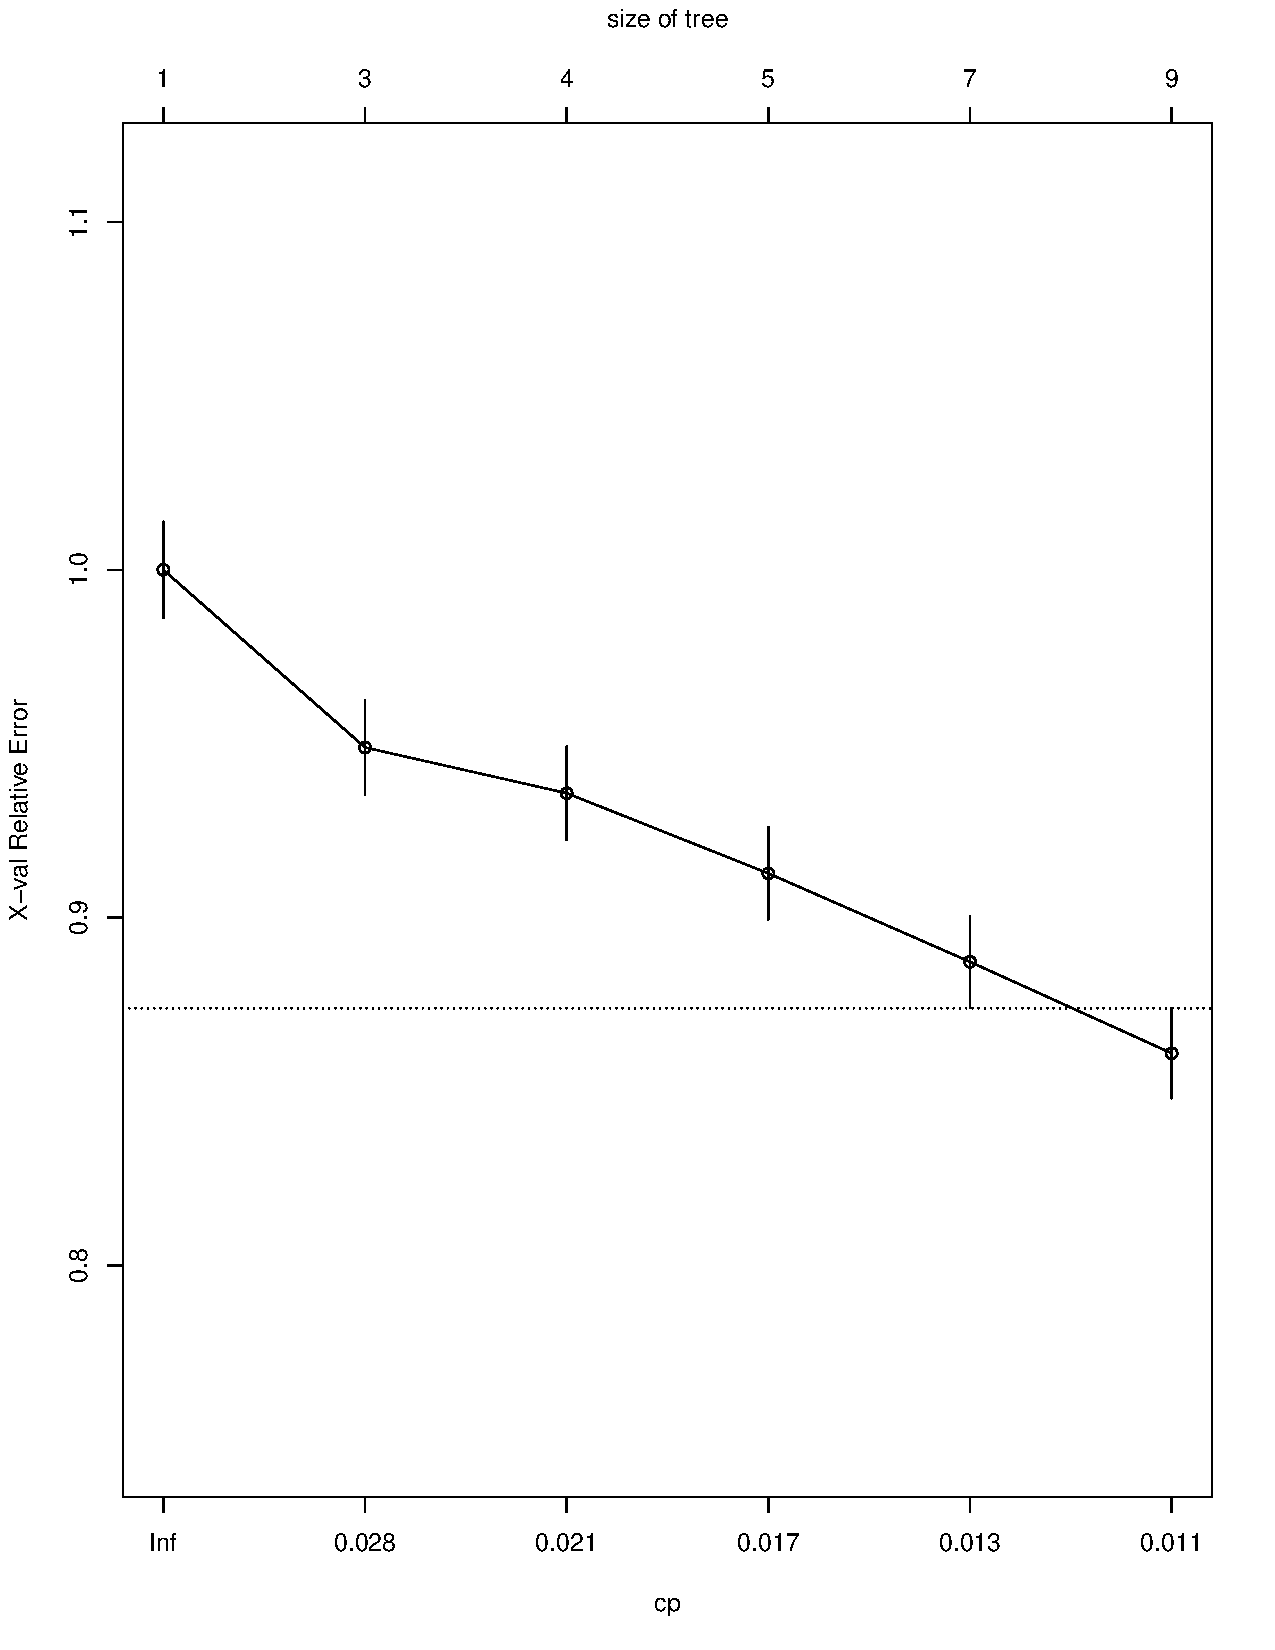
\includegraphics[width=0.7\linewidth]{../MLFBM/decisiontree/plot_cp}
	\caption{plot cross-validation results}
	\label{fig:plotcp}
\end{figure}
\begin{figure}
	\centering
	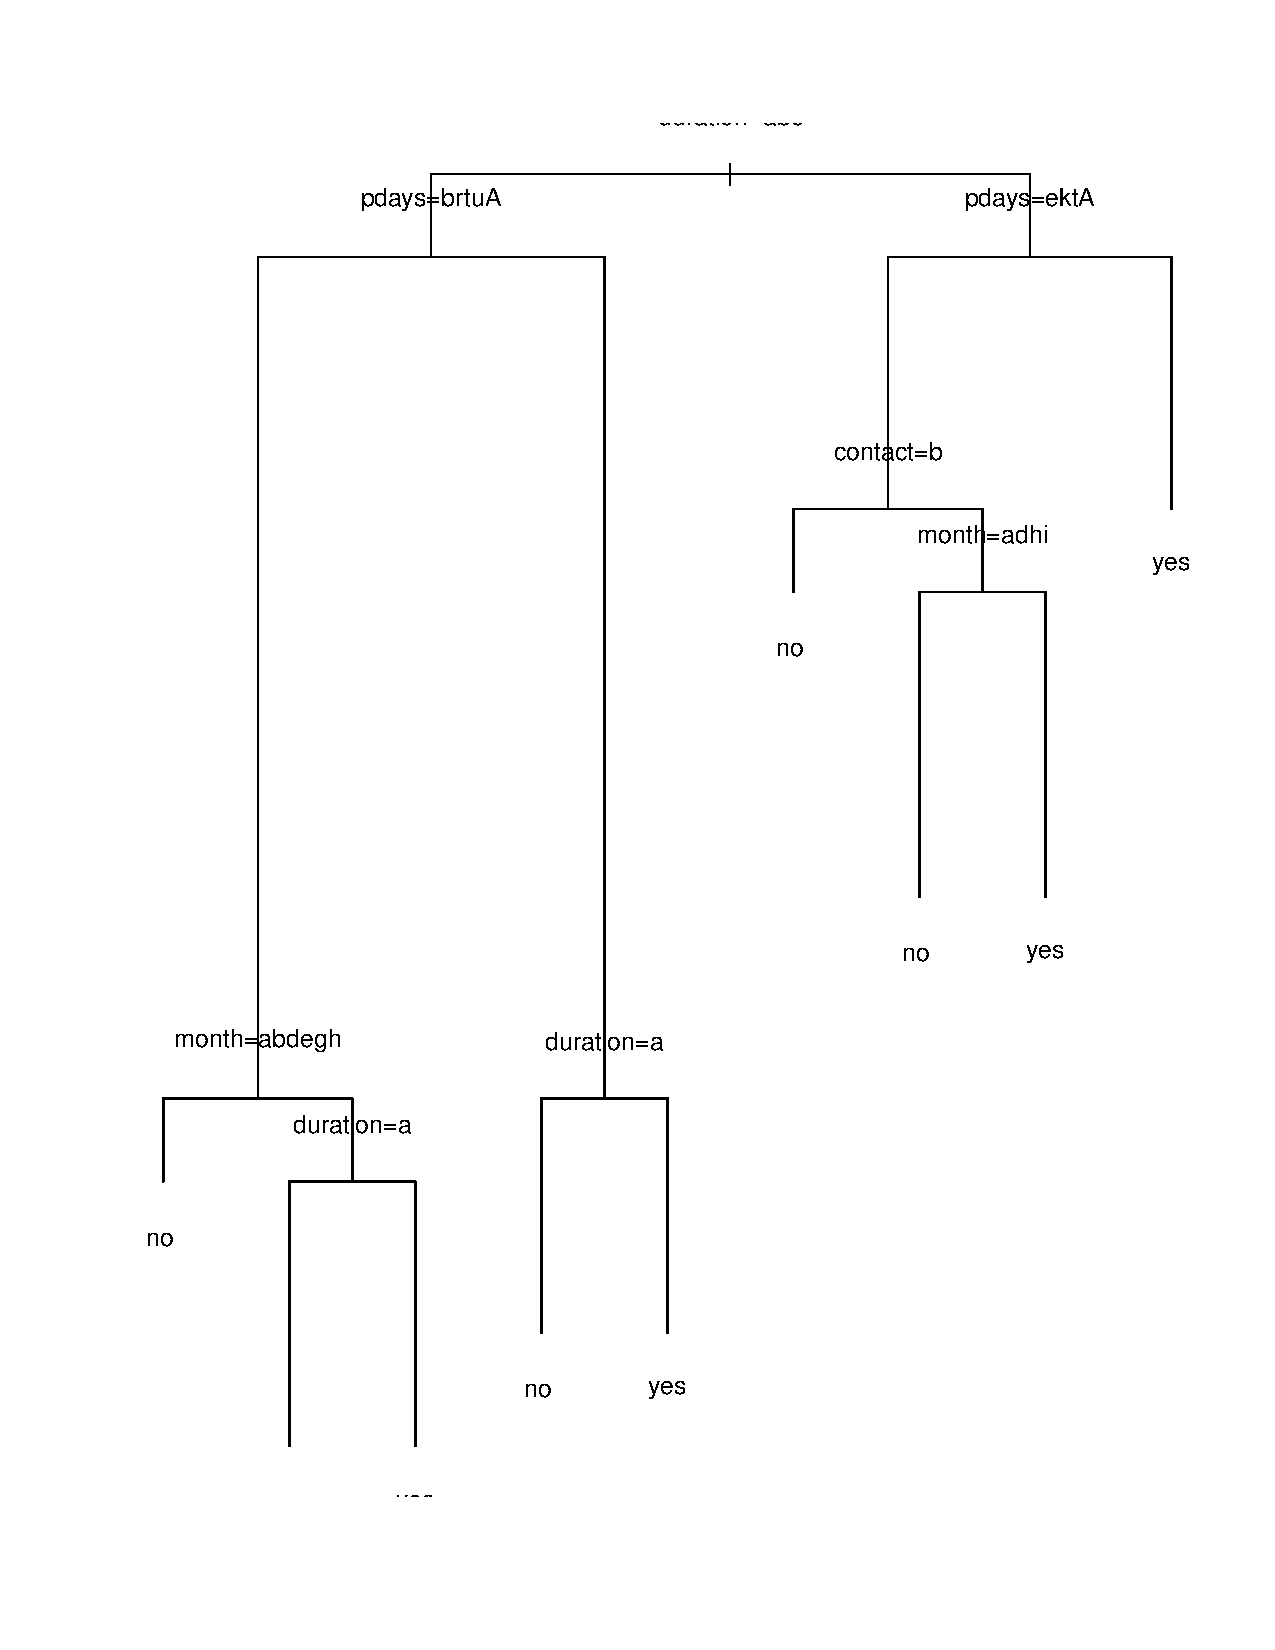
\includegraphics[width=0.7\linewidth]{../MLFBM/decisiontree/plot_pruned_dt}
	\caption{plot pruned tree}
	\label{fig:plotpruneddt}
\end{figure}

\begin{figure}
	\centering
	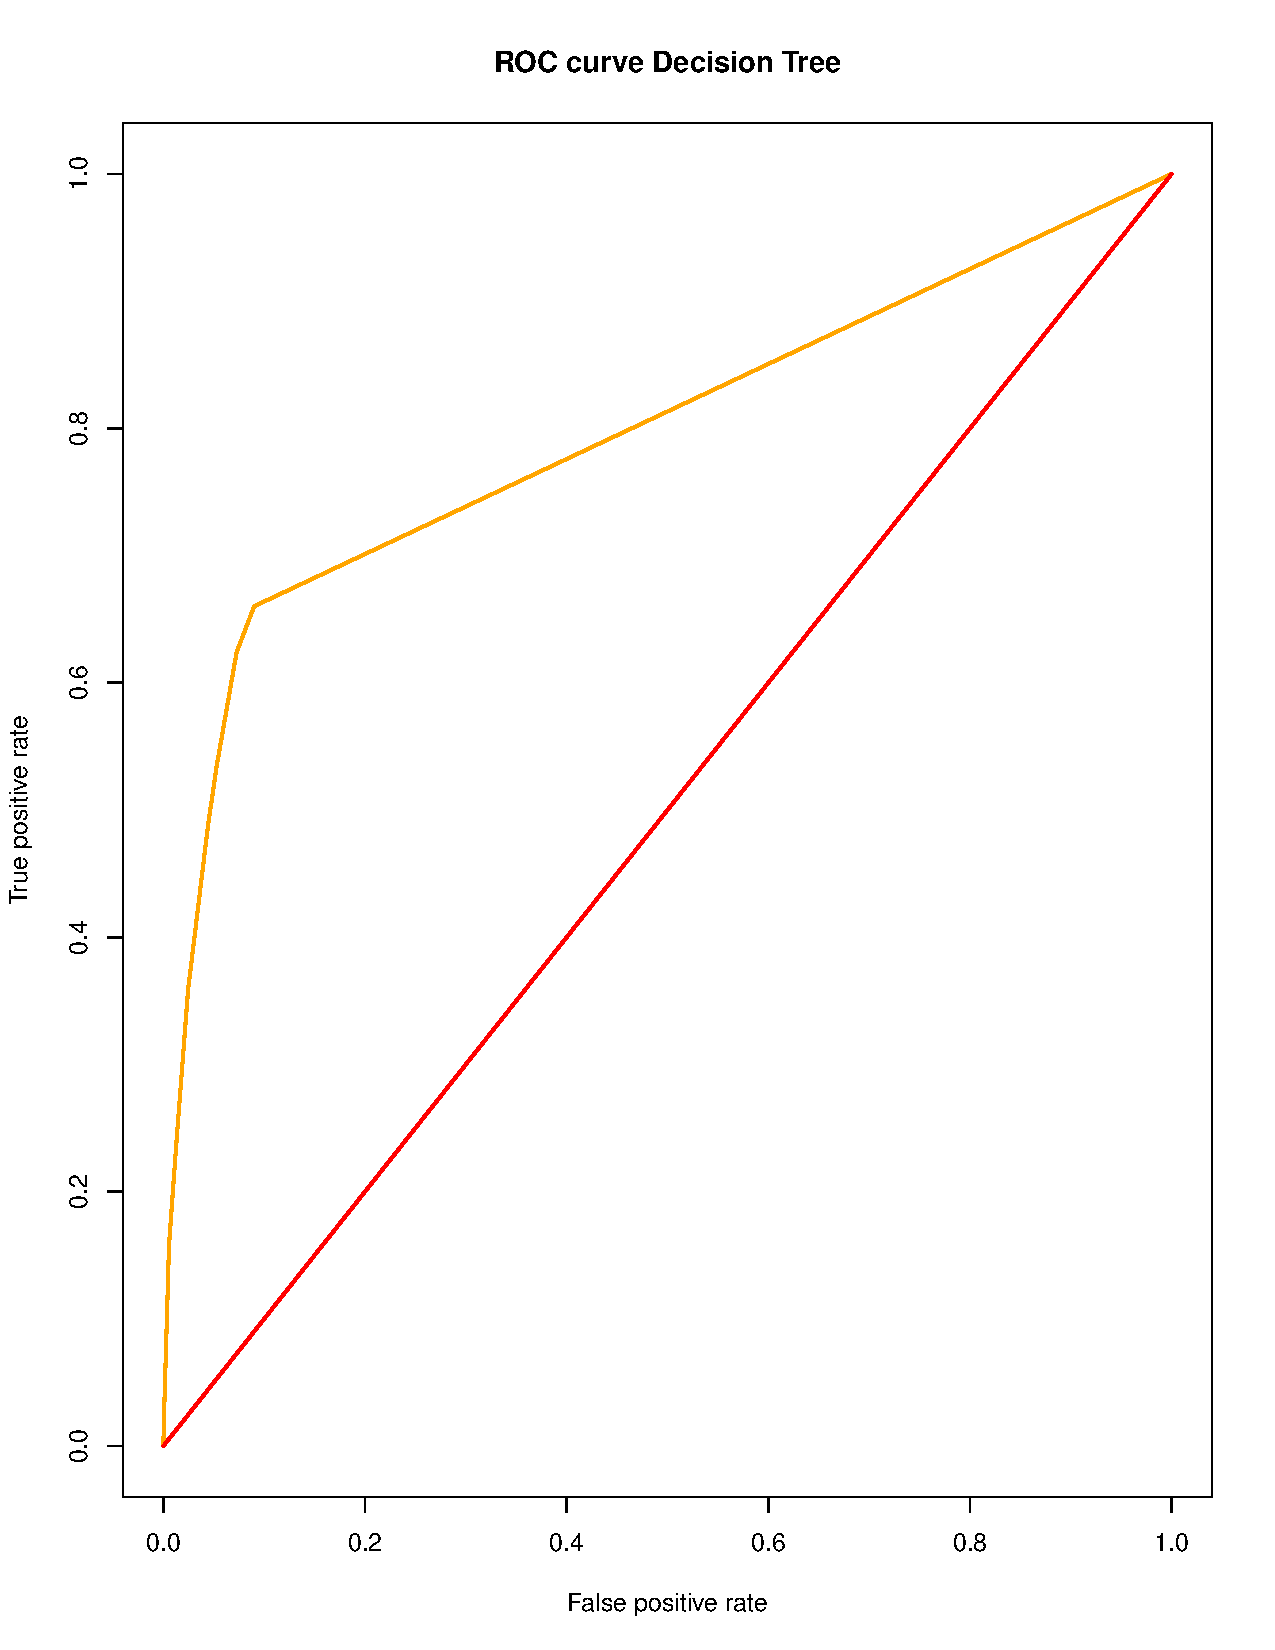
\includegraphics[width=0.7\linewidth]{../MLFBM/decisiontree/ROC_dt}
	\caption{ROC of Decison Tree}
	\label{fig:rocdt}
\end{figure}


%{Random Forest}
\begin{figure}
	\centering
	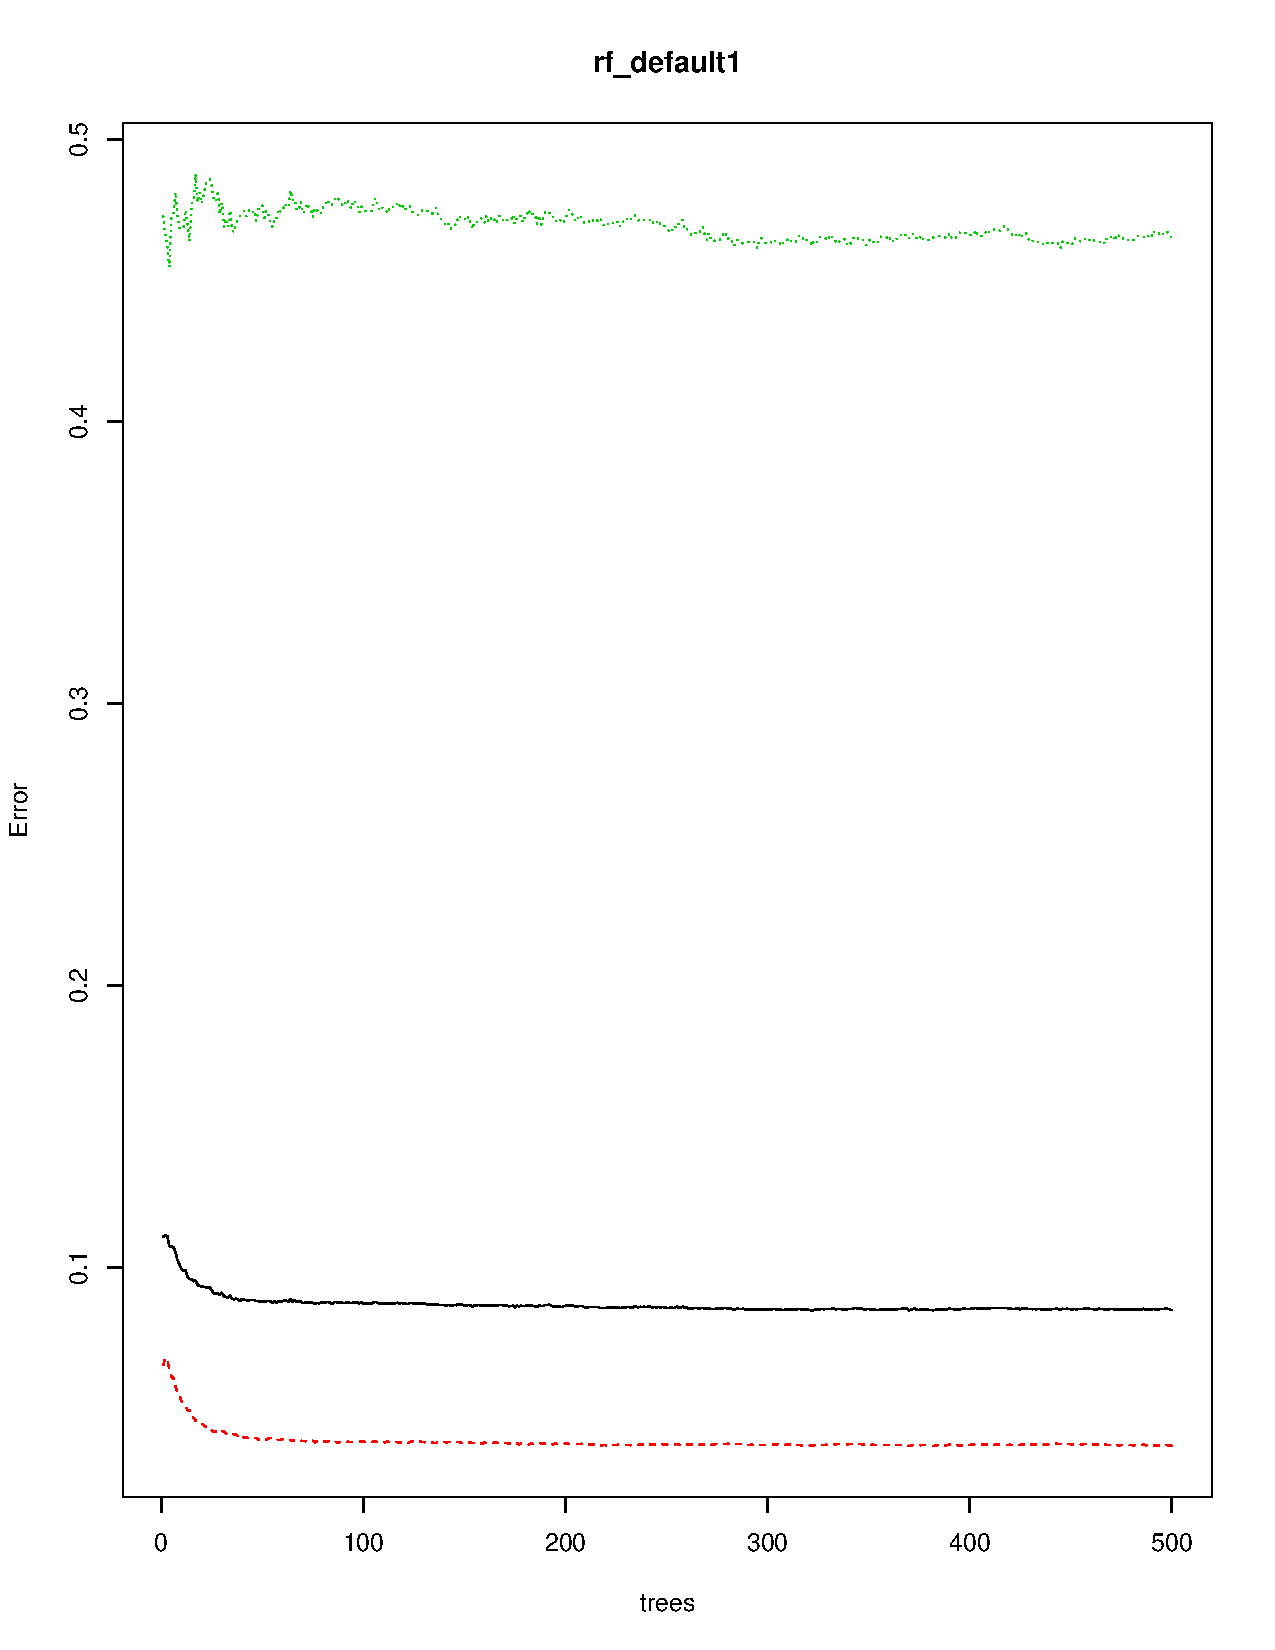
\includegraphics[width=0.7\linewidth]{../MLFBM/RF/RF1}
	\caption{rf\_default1(Random Forest)}
	\label{fig:rf1}
\end{figure}

\begin{figure}
	\centering
	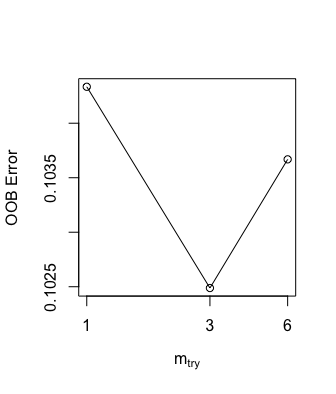
\includegraphics[width=0.7\linewidth]{../MLFBM/RF/RF2}
	\caption{Top 10 − Variable Importance(Random Forest)}
	\label{fig:rf2}
\end{figure}

\begin{figure}
	\centering
	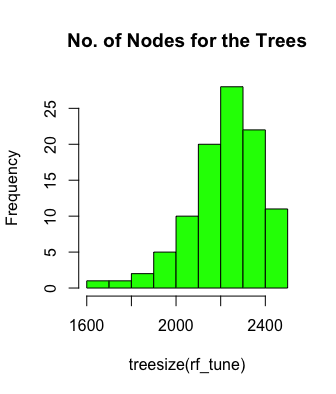
\includegraphics[width=0.7\linewidth]{../MLFBM/RF/RF3}
	\caption{OOB Error(Random Forest)}
	\label{fig:rf3}
\end{figure}

\begin{figure}
	\centering
	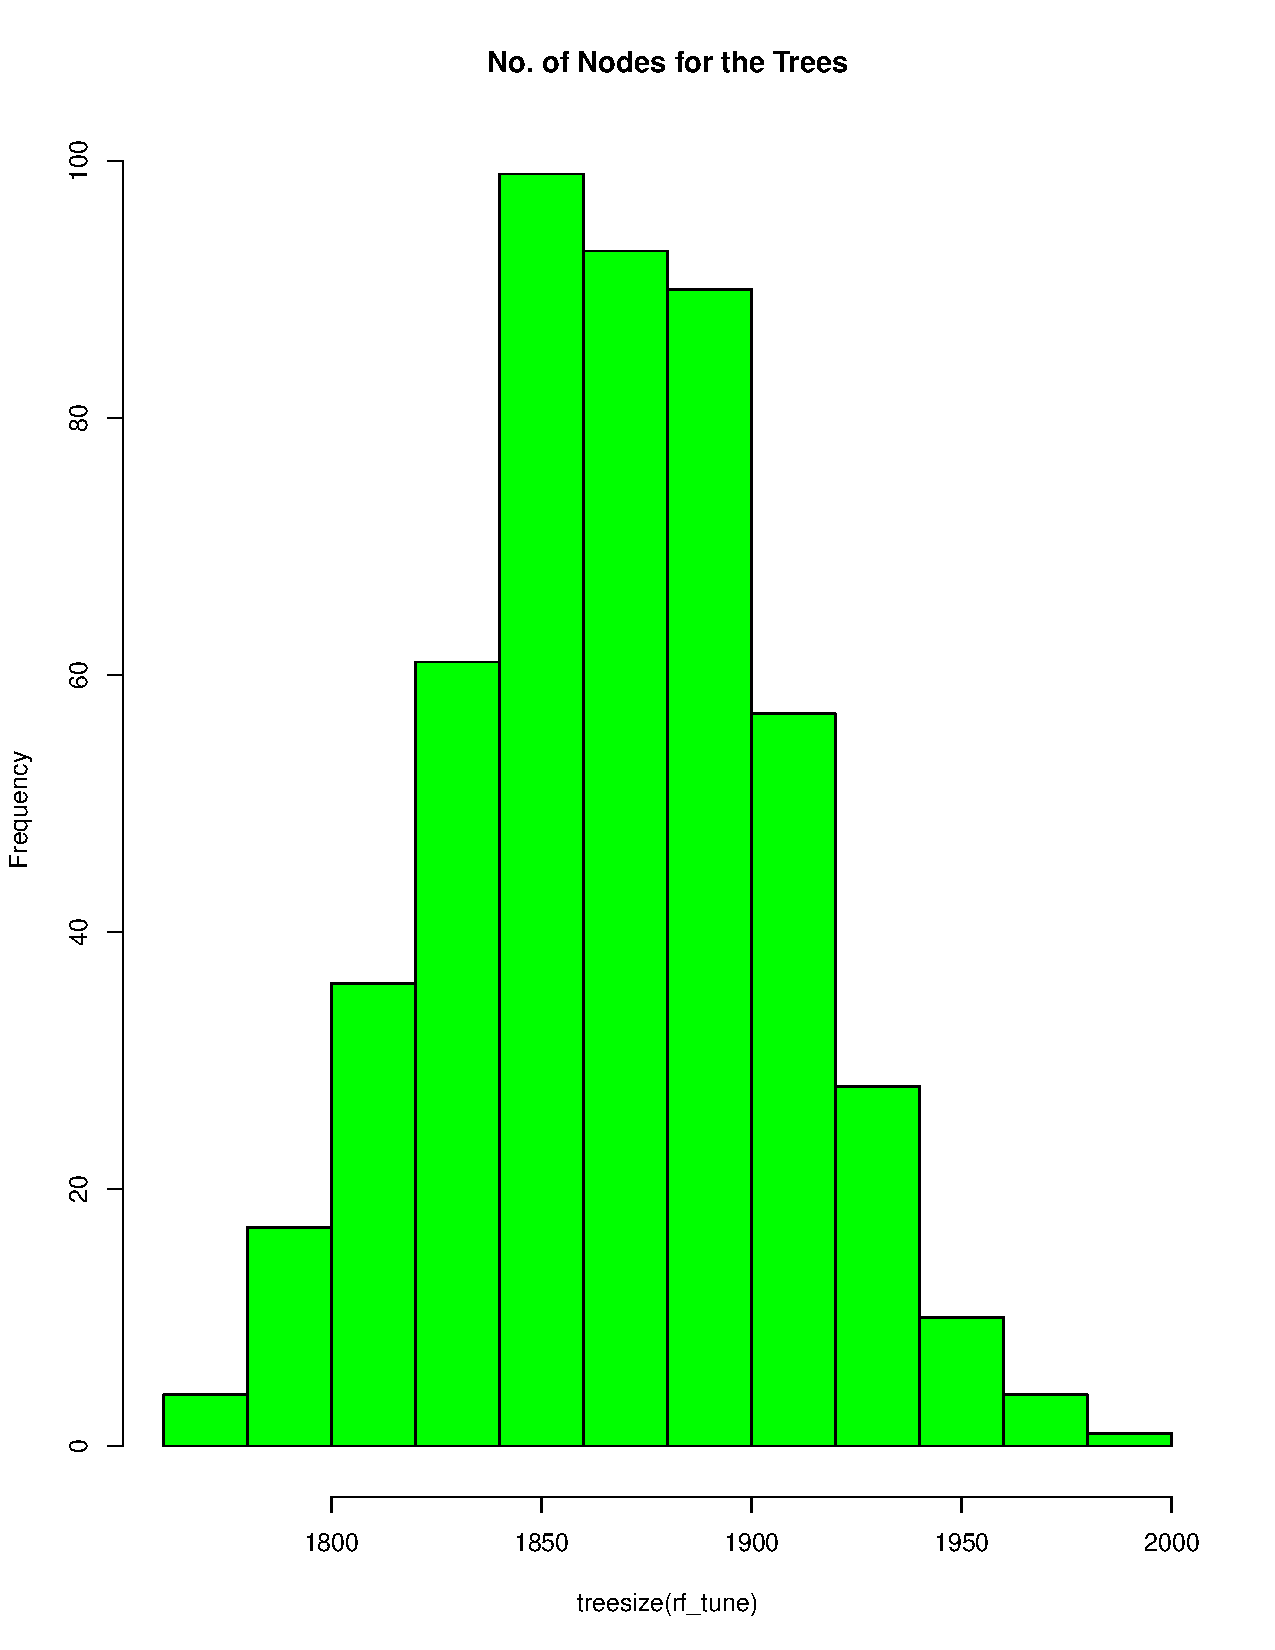
\includegraphics[width=0.7\linewidth]{../MLFBM/RF/RF4}
	\caption{No. of Nodes for the Trees(Random Forest)}
	\label{fig:rf4}
\end{figure}

\begin{figure}
	\centering
	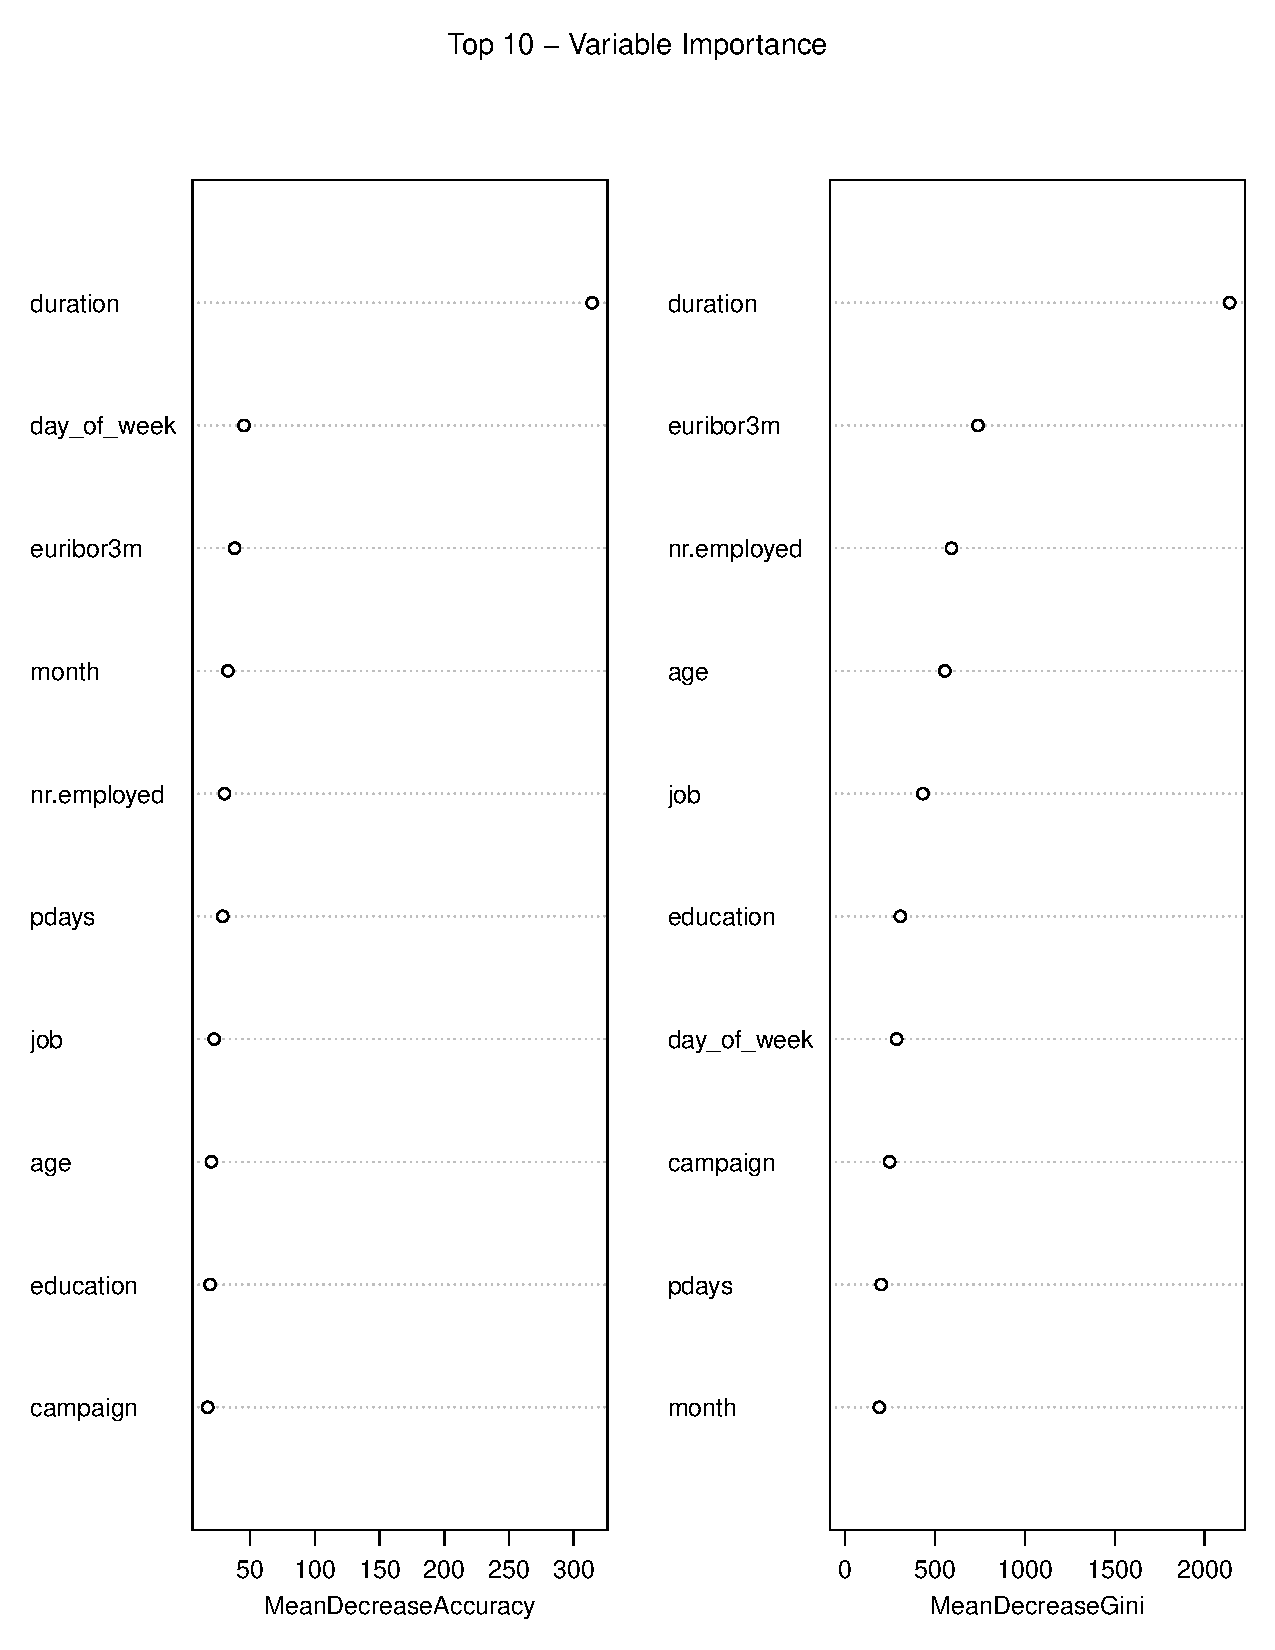
\includegraphics[width=0.7\linewidth]{../MLFBM/RF/RF5}
	\caption{Top 10 − Variable Importance(Random Forest)}
	\label{fig:rf5}
\end{figure}


%{SVM}

%{Neural Network}
\begin{figure}
	\centering
	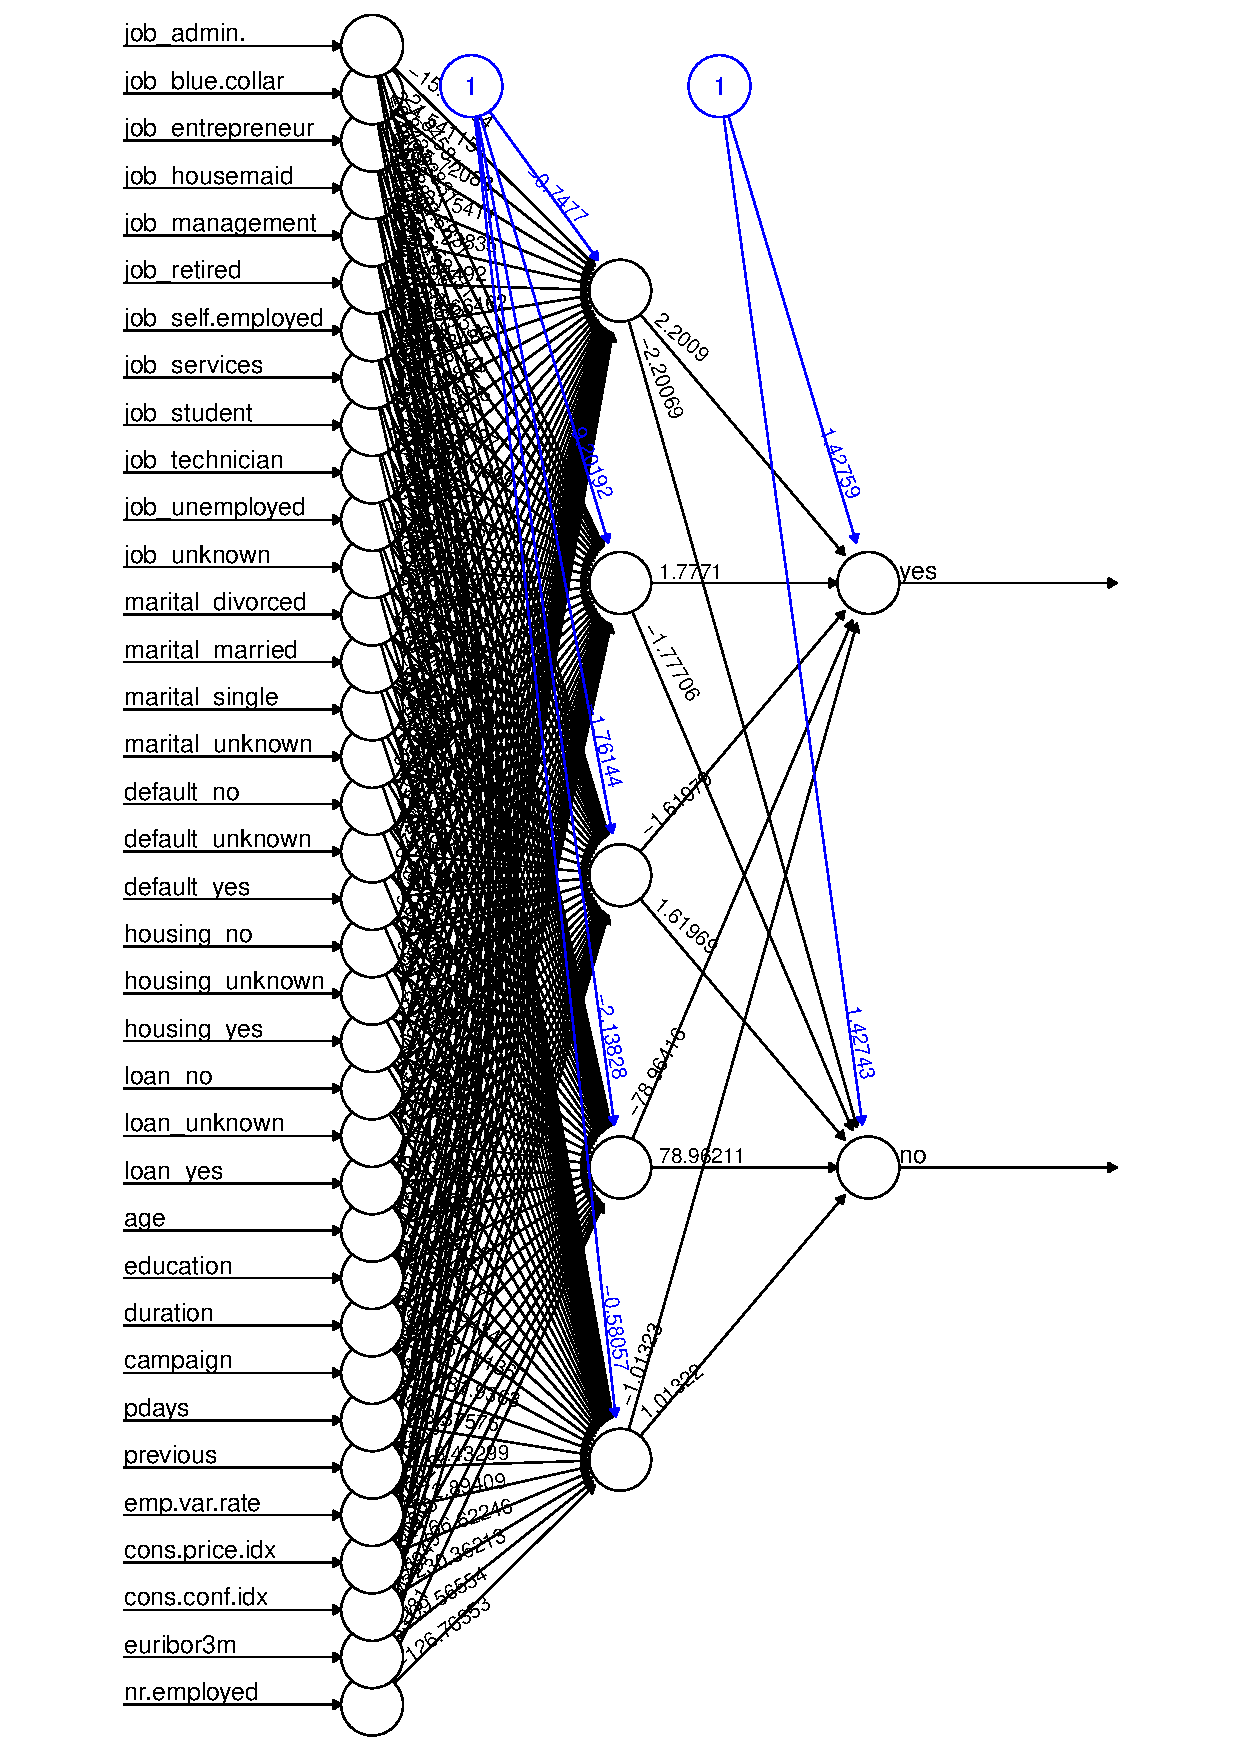
\includegraphics[width=0.7\linewidth]{../MLFBM/NEURALNETPAT/neuralnetworkplot}
	\caption{Neural Network Plot}
	\label{fig:neuralnetworkplot}
\end{figure}

\begin{figure}
	\centering
	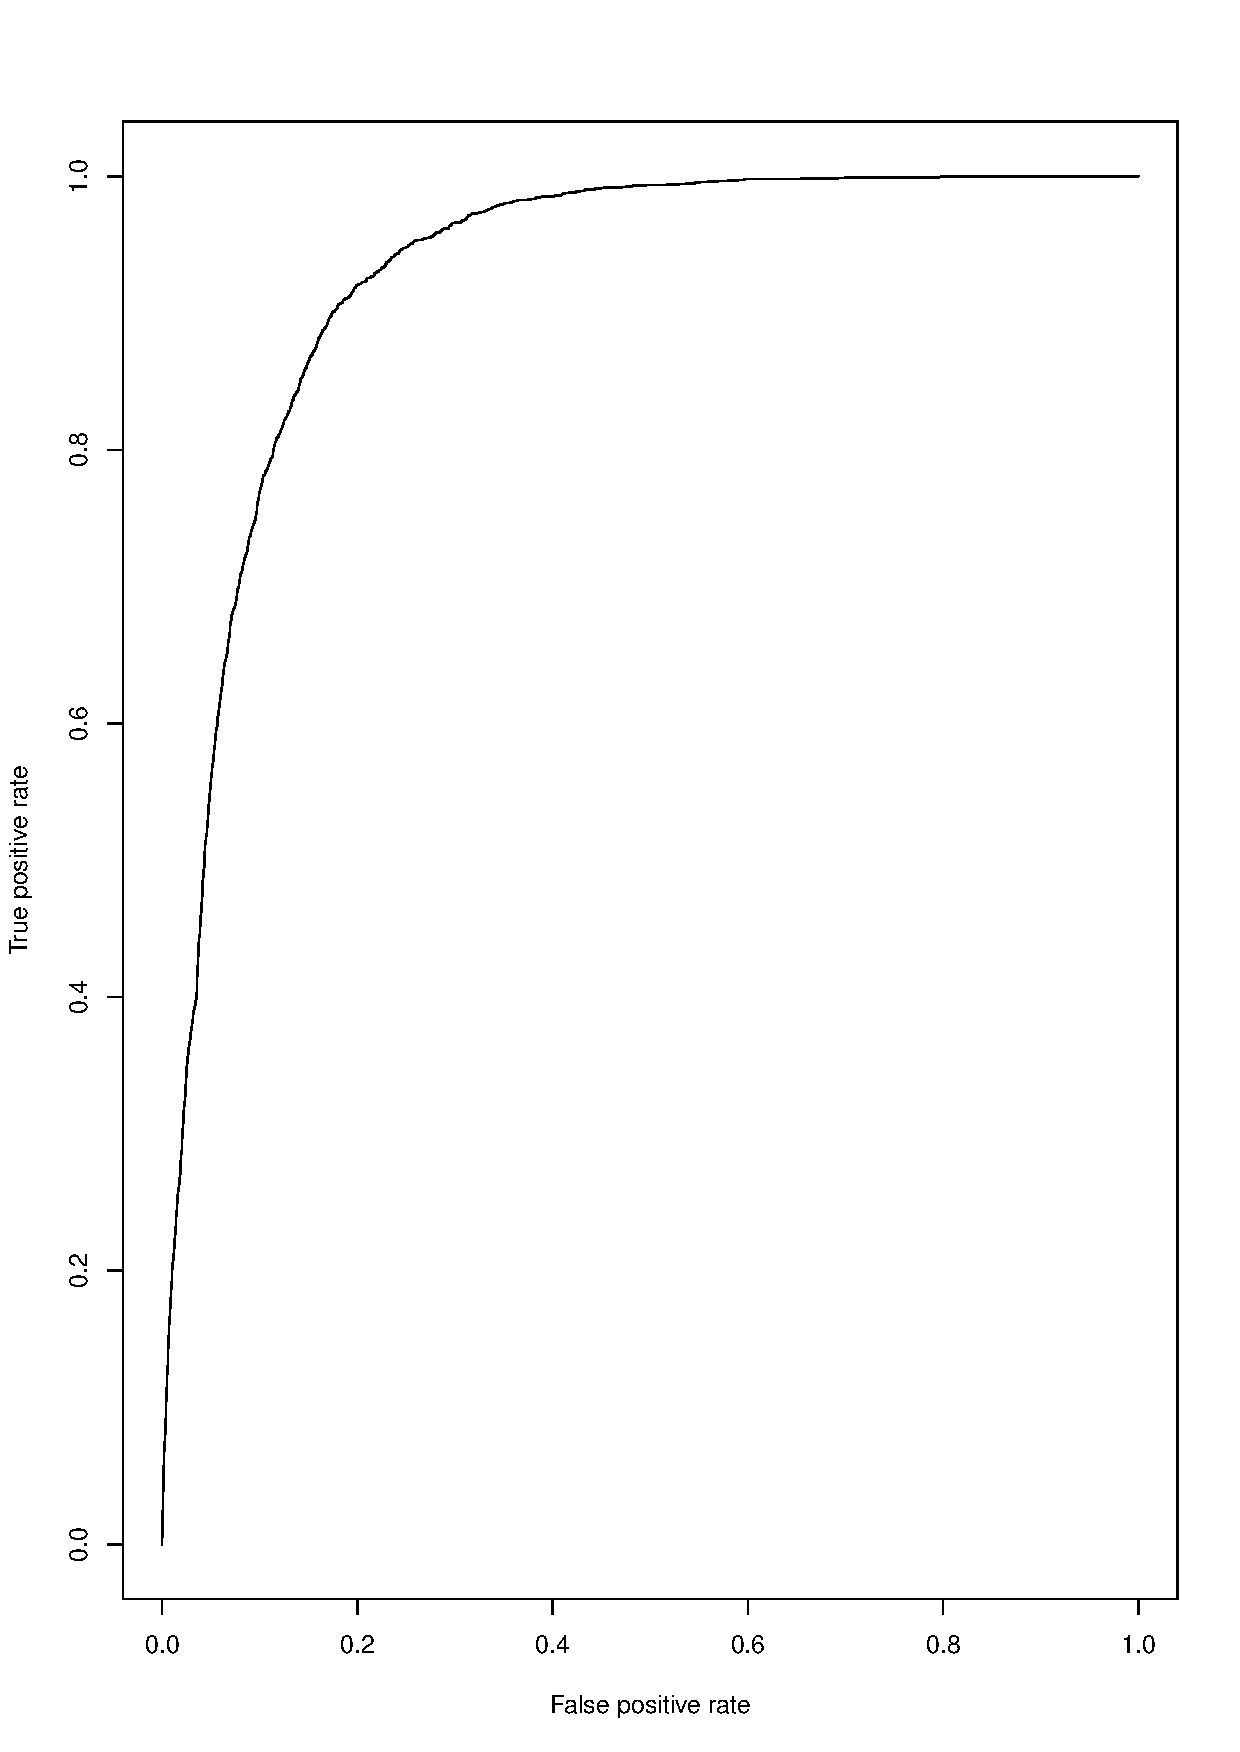
\includegraphics[width=0.7\linewidth]{../MLFBM/NEURALNETPAT/rocplot}
	\caption{ROC of Neural Network}
	\label{fig:rocplot}
\end{figure}

%{Ensemble Selection}
\begin{figure}
	\centering
	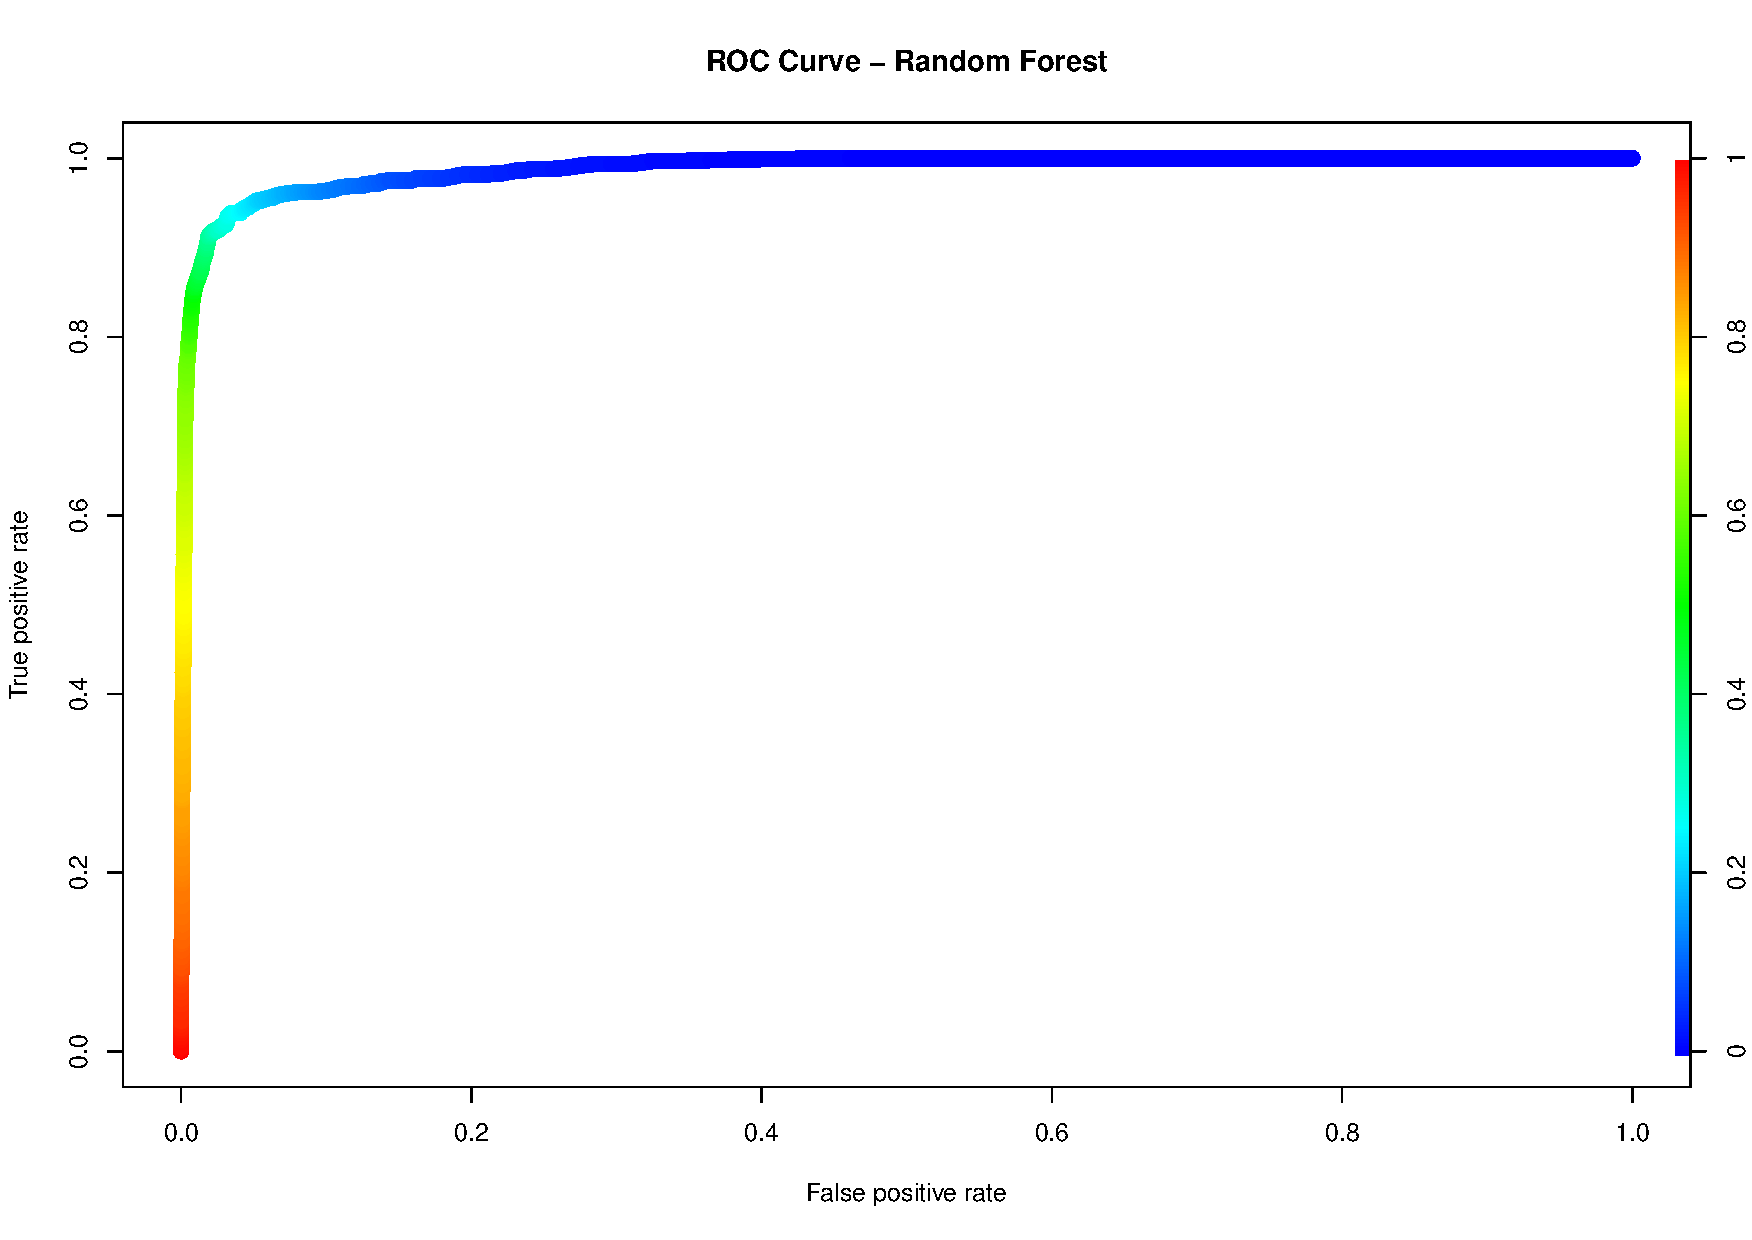
\includegraphics[width=0.7\linewidth]{../MLFBM/ENS/ENS1}
	\caption{ROC Curve − Random Forest(ENS)}
	\label{fig:ens1}
\end{figure}
\begin{figure}
	\centering
	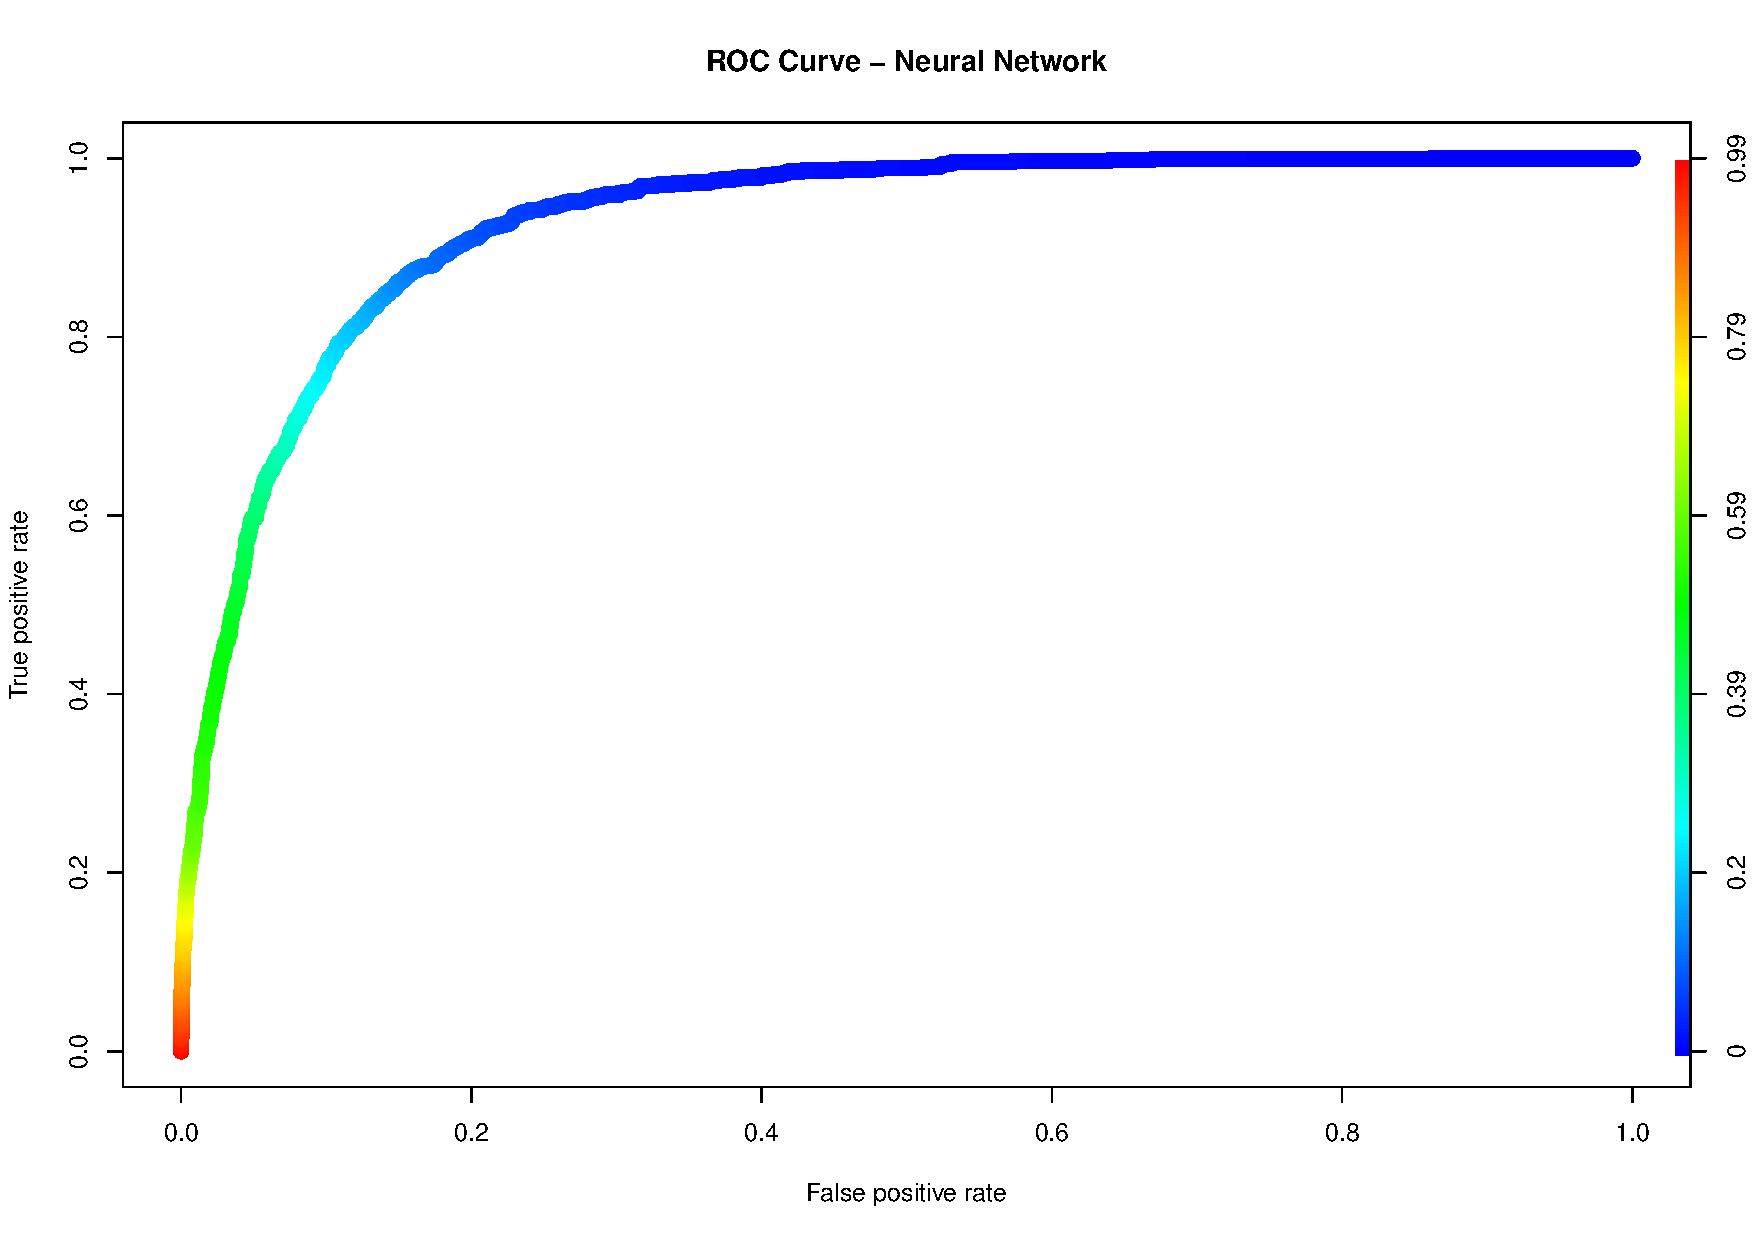
\includegraphics[width=0.7\linewidth]{../MLFBM/ENS/ENS2}
	\caption{ROC Curve − Neural Network(ENS)}
	\label{fig:ens2}
\end{figure}

\begin{figure}
	\centering
	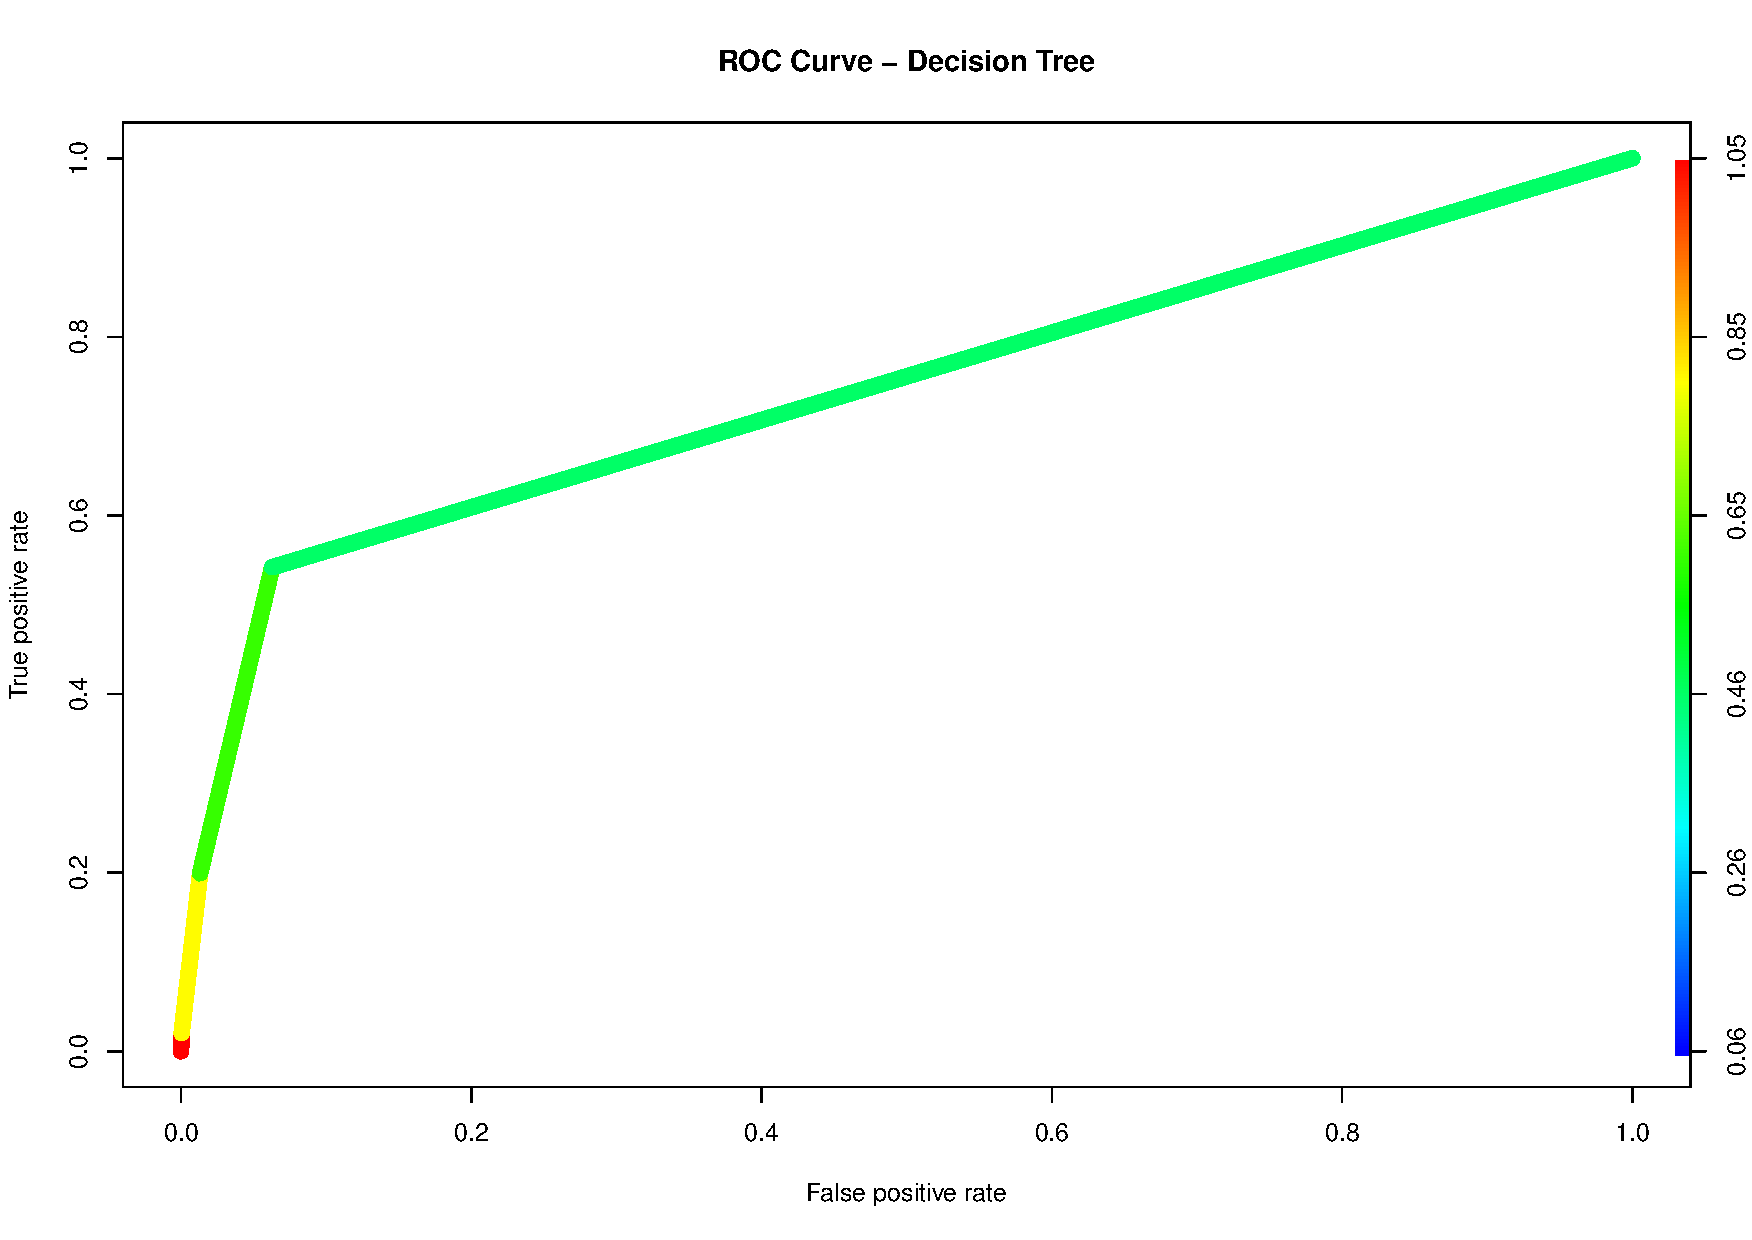
\includegraphics[width=0.7\linewidth]{../MLFBM/ENS/ENS3}
	\caption{ROC Curve − Decision Tree(ENS)}
	\label{fig:ens3}
\end{figure}
\begin{figure}
	\centering
	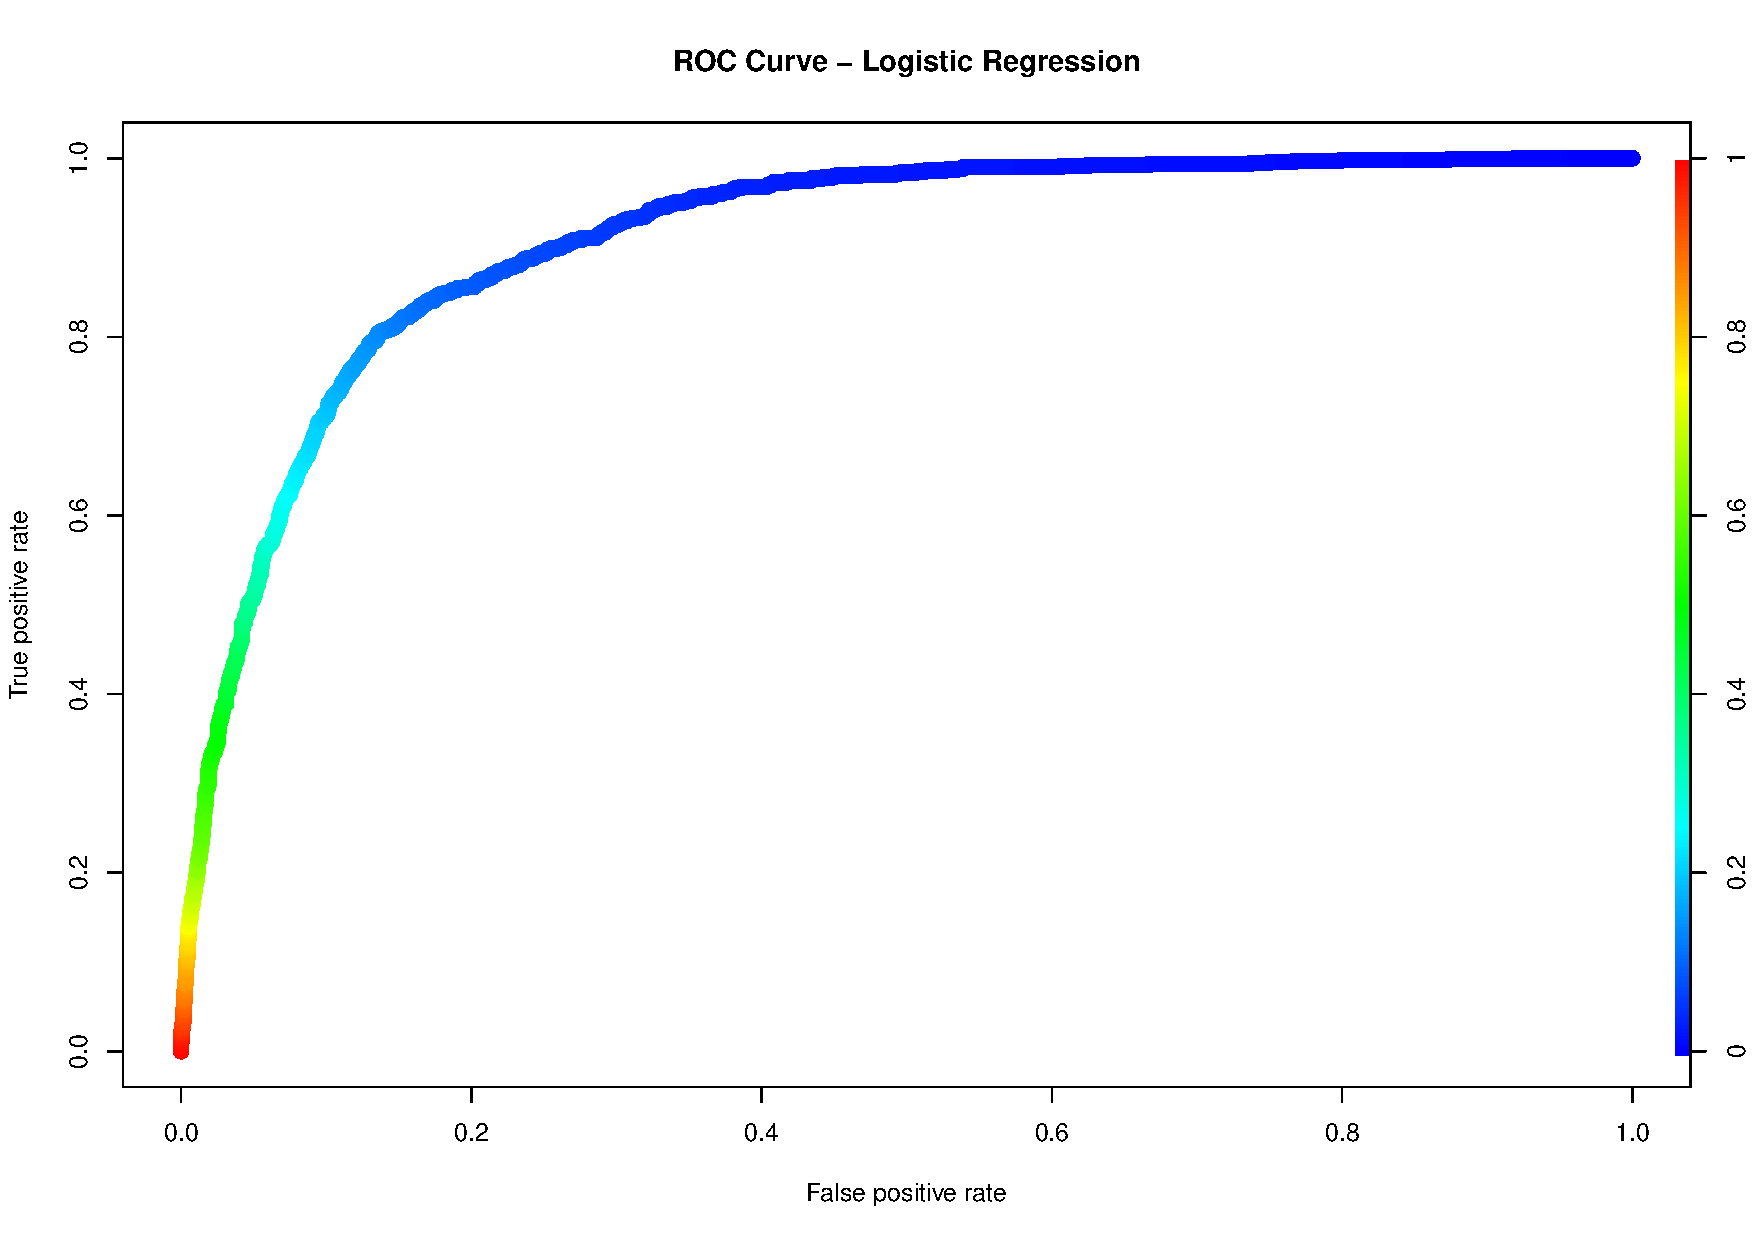
\includegraphics[width=0.7\linewidth]{../MLFBM/ENS/ENS4}
	\caption{ROC Curve − Logistic Regression(ENS)}
	\label{fig:ens4}
\end{figure}


\printbibliography

\addsec{Declaration of Authorship}

We hereby confirm that we have authored this Seminar paper independently and without use of others than the indicated sources. All passages which are literally or in general matter taken out of publications or other sources are marked as such.



\emph{City}            \begin{flushright}
	Berlin\\
\end{flushright}

\emph{Date}            \begin{flushright}
	18.08.2017\\
\end{flushright}

\emph{Name of Group members}\\
\begin{flushright}
	Zhou \textsc{Ren}\\
	Jingyi \textsc{Liu}\\
	Manqi \textsc{Ding}\\
	Jiayin \textsc{Yuan}
\end{flushright}


\bibliographystyle{plain}
\bibliography{litnew}




\end{document}
